%%%%%%%%%%%%%%%%%%%%%%%%%%%%%%%%%%%%%%%%%%%%%%%%%%%
%
%  New template code for TAMU Theses and Dissertations starting Fall 2012.  
%  For more info about this template or the 
%  TAMU LaTeX User's Group, see http://www.howdy.me/.
%
%  Author: Wendy Lynn Turner 
%	 Version 1.0 
%  Last updated 8/5/2012
%
%%%%%%%%%%%%%%%%%%%%%%%%%%%%%%%%%%%%%%%%%%%%%%%%%%%
%%%   Chapter - DSA
%%%%%%%%%%%%%%%%%%%%%%%%%%%%%%%%%%%%%%%%%%%%%%%%%%%
\chapter{\uppercase {Diffusion Synthetic Acceleration for Discontinuous Finite Elements on Unstructured Grids}}
\label{sec::DSA}

%%%%%%%%%%%%%%%%%%%%%%%%%%%%%%%%%%%%%%%%%%%%%%%%%%%
%%%%%%%%%%%%%%%%%%%%%%%%%%%%%%%%%%%%%%%%%%%%%%%%%%%
%%%   Section - Introduction
%%%%%%%%%%%%%%%%%%%%%%%%%%%%%%%%%%%%%%%%%%%%%%%%%%%
%%%%%%%%%%%%%%%%%%%%%%%%%%%%%%%%%%%%%%%%%%%%%%%%%%%
\section{Introduction}
\label{sec::DSA_Introduction}

In this chapter, we analyze the Modified Interior Penalty (MIP) form of the diffusion equation as a discretization scheme for use with Diffusion Synthetic Acceleration (DSA) of the DFEM $S_N$ transport equation on unstructured grids. Specifically, we wish to analyze its efficacy on massively-parallel computer architectures where scalability of solution times and memory footprints can become burdensome. This chapter is laid out in the following manner. The remainder of this Section will provide an overview of synthetic acceleration techniques as well as a review of DSA schemes. Section \ref{sec::DSA_DSA} provides the DSA methodologies that we will employ for 1-group and thermal neutron upscattering acceleration. We then present the discontinuous Symmetric Interior Penalty (SIP) form of the diffuion equation in Section \ref{sec::DSA_SIP} as well as the MIP variant that we will use for our DSA analysis in Section \ref{sec::DSA_MIP}. The numerical procedures that we will use to solve the diffusion system of equations is given in Section \ref{sec::DSA_Solving}. The theoretical Fourier analysis tool is given in Section \ref{sec::DSA_Fourier}. Results are provided in Section \ref{sec::DSA_Results} and we finish the chapter with some concluding remarks in Section \ref{sec::DSA_Conclusions}

%%%%%%%%%%%%%%%%%%%%%%%%%%%%%%%%%%%%%%%%%%%%%%%%%%%
%%%%%%%%%%%%%%%%%%%%%%%%%%%%%%%%%%%%%%%%%%%%%%%%%%%
%%%   SubSection - History
\subsection{Review of Diffusion Synthetic Accleration Schemes}
\label{sec::DSA_Introduction_History}

cleanup the beginning here later...

The ability to efficiently invert the transport (streaming and collision) operator does not necessarily mean that transport solutions can be easily obtained. In general, radiation transport solutions are obtained iteratively. The simplest and widely-used method is a fixed-point scheme ({\em i.e.} richardson iteration) ubiquitously called source iteration (SI) in the transport community. Unfortunately, the iteration process of SI can converge arbitrarily slowly if the problem is optically thick \cite{ref::adams_larsen_iter_methods}. This corresponds to long mean free paths for neutronics problems. This also corresponds to time steps and material heat capacities tending to infinity and zero, respectively, for thermal radiative transport (TRT) problems.

For these problem regimes in which solution is prohibitively slow, additional steps should be taken to speed up, or accelerate, solution convergence \cite{ref::adams_larsen_iter_methods}. The most used methods to assist in solution convergence are often called synthetic acceleration techniques. These techniques were first introduced by Kopp \cite{kopp1963synthetic} and Lebedev \cite{lebedevI,lebedevII,lebedevIII,lebedevIV,lebedevV,lebedevVI,lebedevVII} in the 1960's. From Kopp's and Lebedev's work, Gelbard and Hageman then introduced two synthetic acceleration options for the low-order operator: diffusion and $S_2$ \cite{gelbard1969synthetic}. Their diffusion preconditioning led to efficient convergence properties on fine spatial meshes. Reed then showed that Gelbard and Hageman's diffusion preconditioning would yield a diverging system for coarse meshes \cite{reed1971effectiveness}. At this point in time, no one knew if an unconditionally efficient acceleration method could be derived.

Then in 1976, Alcouffe proposed a remedy to Gelbard and Reed that he called diffusion synthetic acceleration (DSA) \cite{alcouffe1976stable,alcouffe1977DSA,alcouffe1977diffusion}. He showed that if you derived the diffusion operator consistently with the discretized transport operator, then SI could be accelerated with DSA in an efficient and robust manner. Larsen and McCoy then demonstrated that unconditional stability required that consistency be maintained in both spatial and angular discretization in their four-step procedure \cite{larsen1982unconditionally_I,larsen1982unconditionally_II}. However, Adams and Martin then showed that partially-consistent diffusion discretizations could effectively accelerate DFEM discretizations of the neutron transport equation \cite{ref::dsa_DFEM_adams_martin}. Their modified-four-step procedure (M4S), based on Larsen and McCoy's work, was shown to be unconditionally stable for regular geometries, but divergent for unstructured multi-dimensional meshes \cite{warsa2002fully}. In more recent years, alternate discretizations for the diffusion operator have been applied to unstructured multi-dimensional grids. These include the partially consistent Wareing-Larsen-Adams (WLA) DSA \cite{ref::WLA_DSA}, the fully consistent DSA (FCDSA) \cite{warsa2002fully}, and the partially consistent MIP DSA \cite{ref::DSA_wang_ragusa,wang2009adaptive,turcksin2014discontinuous}.

Most recently, the partially consistent MIP DSA method has been shown to be an unconditionally stable acceleration method for the 2D DFEM transport equation on unstructured meshes. Wang showed that it acted as an effective preconditioner for higher-order DFEM discretizations on triangles \cite{ref::DSA_wang_ragusa,wang2009adaptive}. Turcksin and Ragusa then extended the work to arbitrary polygonal meshes \cite{turcksin2014discontinuous}. The MIP diffusion operator is symmetric positive definite (SPD) and was shown to be efficiently invertible with preconditioned conjugate gradient (PCG) and advanced preconditioners such as algebraic multi-grid (AMG) \cite{turcksin2014discontinuous}.

%%%%%%%%%%%%%%%%%%%%%%%%%%%%%%%%%%%%%%%%%%%%%%%%%%%
%%%%%%%%%%%%%%%%%%%%%%%%%%%%%%%%%%%%%%%%%%%%%%%%%%%
%%%   SubSection - Synthetic Acceleration
\subsection{Synthetic Acceleration Overview}
\label{sec::DSA_Introduction_SA}

Synthetic acceleration techniques have been widely used in the nuclear engineering community to improve solution convergence for prohibitively slow problems. We now provide a general framework for how synthetic acceleration methods are derived. We begin by expressing our neutron transport equation in the following form,

\begin{equation}
\label{eq::DSA_simple_trans_eq_w_ops}
\left(  {\bf A} - {\bf B}  \right) \Psi = {\bf Q} ,
\end{equation}

\noindent where ${\bf A}$ and ${\bf B}$ are both linear operators, $\Psi$ is the full angular flux solution in space, angle, and energy, and ${\bf Q}$ is the source or driving function. If we had the ability to efficiently invert $\left(  {\bf A} - {\bf B}  \right)$ directly, then $\Psi$ could be directly computed:

\begin{equation}
\label{eq::DSA_simple_trans_eq_w_ops_inverted}
\Psi = \left(  {\bf A} - {\bf B}  \right)^{-1} {\bf Q} .
\end{equation}

\noindent However, since in practice the discretized version of $\left(  {\bf A} - {\bf B}  \right)$ is much more costly to directly invert than the discretized version of ${\bf A}$, we instead choose to iteratively solve for $\Psi$.

To compute $\Psi$, the following iterative system of equations is usually employed,

\begin{equation}
\label{eq::DSA_simple_trans_eq_w_ops_iterates}
 {\bf A} \Psi^{(k+1)} - {\bf B}  \Psi^{(k)} = {\bf Q} ,
\end{equation}

\noindent where directly solving for $\Psi^{(k+1)}$ yields the following:

\begin{equation}
\label{eq::DSA_simple_trans_eq_sol_w_ops_iterates}
 \Psi^{(k+1)} =  {\bf A}^{-1} {\bf B}  \Psi^{(k)} +  {\bf A}^{-1} {\bf Q} .
\end{equation}

\noindent For brevity, we define a new operator ${\bf C} = {\bf A}^{-1} {\bf B}$ which is known as the iteration operator. The spectral radius, $\rho$, of this operator is simply the supremum of the absolute values of its eigenvalues. For this work, we assume that $\rho$ is less than unity to guarantee convergence. We next define the residual, $r^{(k)}$, as the difference between two successive solution iterates,

\begin{equation}
\label{eq::DSA_synthetic_eq_residual}
r^{(k)} = \Psi^{(k)} - \Psi^{(k-1)} ,
\end{equation}

\noindent which can also be written as the following:

\begin{equation}
\label{eq::DSA_synthetic_eq_residual_op}
r^{(k)} = {\bf C}\Psi^{(k-1)} .
\end{equation}

With the iteration operator, ${\bf C}$, and the residual for iterate $k$ , $r^{(k)}$, defined, we can then write the true, converged solution in terms of the solution at iteration $k$ and an infinite series of residuals:

\begin{equation}
\label{eq::DSA_synthetic_eq_true_sol}
\Psi = \Psi^{(k)} + \sum_{n=1}^{\infty} r^{(k+n)} .
\end{equation}

\noindent Using both Eqs. (\ref{eq::DSA_synthetic_eq_residual_op}) and (\ref{eq::DSA_synthetic_eq_true_sol}), we can rewrite Eq. (\ref{eq::DSA_synthetic_eq_true_sol}) using the iteration operator and the last residual,

\begin{equation}
\label{eq::DSA_synthetic_eq_true_sol_it_op}
\Psi = \Psi^{(k)} + \left(  {\bf I} + {\bf C} + {\bf C}^2 + ...  \right) {\bf C} r^{(k)}.
\end{equation}

\noindent Since we have assumed that the spectral radius of {\bf C} is less than unity, the infinite operator series of Eq. (\ref{eq::DSA_synthetic_eq_true_sol_it_op}) converges to $\left(  {\bf I} - {\bf C}   \right)^{-1} {\bf C}$. This means that we can succinctly write Eq. (\ref{eq::DSA_synthetic_eq_true_sol_it_op}) as the following:

\begin{equation}
\label{eq::DSA_synthetic_eq_true_sol_it_op_succinct}
\Psi = \Psi^{(k)} + \left(  {\bf I} - {\bf C}   \right)^{-1} {\bf C} r^{(k)}.
\end{equation}

\noindent By using the definition of ${\bf C}$ along with some linear algebra, Eq. (\ref{eq::DSA_synthetic_eq_true_sol_it_op_succinct}) becomes 

\begin{equation}
\label{eq::DSA_synthetic_eq_true_sol_orig_ops}
\Psi = \Psi^{(k)} + \left(  {\bf A} - {\bf B}   \right)^{-1} {\bf B} r^{(k)}.
\end{equation}

We would like to use the results of Eq. (\ref{eq::DSA_synthetic_eq_true_sol_orig_ops}) to immediately compute our exact transport solution, $\Psi$. However, this would require the inversion of $\left(  {\bf A} - {\bf B}  \right)$ which we did not employ originally in Eq. (\ref{eq::DSA_simple_trans_eq_w_ops}) because of the difficulty. This means that, in its current form, Eq. (\ref{eq::DSA_synthetic_eq_true_sol_orig_ops}) is no more useful to us than Eq. (\ref{eq::DSA_simple_trans_eq_w_ops}). This would then be an exercise in futility if we were restricted to only working with the $\left(  {\bf A} - {\bf B}  \right)$ operator. Instead, suppose that we could define an operator, ${\bf W}$, that closely approximates $\left(  {\bf A} - {\bf B}  \right)$ but it is easily invertible. If ${\bf W}$ efficiently approximates the slowest converging error modes of $\left(  {\bf A} - {\bf B}  \right)$, then Eq. (\ref{eq::DSA_synthetic_eq_true_sol_orig_ops}) can be modified to form a new iterative procedure.

The new iterative procedure begins by simply taking the half-iterate of Eq. (\ref{eq::DSA_simple_trans_eq_sol_w_ops_iterates}) instead of its full version: ${(k+1/2)}$ instead of {(k+1)}. This half-iterate has the form

\begin{equation}
\label{eq::DSA_synthetic_eq_half_it}
\Psi^{(k+1/2)} = {\bf C} \Psi^{(k)} + {\bf A}^{-1} {\bf Q}.
\end{equation}

\noindent We can then express the full-iterate by the suggestion of Eq. (\ref{eq::DSA_synthetic_eq_true_sol_orig_ops}). Using the low-order operator, we express the full-iterate as the following,

\begin{equation}
\label{eq::DSA_synthetic_eq_half_it_correction}
\Psi^{(k+1)} =\Psi^{(k+1/2)} + {\bf W}^{-1} {\bf B}  r^{(k+1/2)},
\end{equation}

\noindent where $r^{(k+1/2)} = \Psi^{(k+1/2)} - \Psi^{(k)}$. We can also express Eq. (\ref{eq::DSA_synthetic_eq_half_it_correction}) in terms of just the previous iterate, $\Psi^{(k)}$, and a new operator:

\begin{equation}
\label{eq::DSA_synthetic_eq_new_algo}
\Psi^{(k+1)} = \left[  {\bf I} - {\bf W}^{-1} \left(  {\bf A} - {\bf B}  \right)  \right] {\bf C} \Psi^{(k)} + \left({\bf I} + {\bf W}^{-1} {\bf B} \right) {\bf A}^{-1} {\bf Q} .
\end{equation}

\noindent Observe that as ${\bf W}$ more closely approximates $\left(  {\bf A} - {\bf B}  \right)$, the operator ${\bf W}^{-1} \left(  {\bf A} - {\bf B}  \right)$ converges to the identity matrix, ${\bf I}$. This means that the spectral radius of this new iteration matrix will approach zero as ${\bf W}$ gets closer to $\left(  {\bf A} - {\bf B}  \right)$ and therefore more quickly and efficiently converge to the true solution.

%%%%%%%%%%%%%%%%%%%%%%%%%%%%%%%%%%%%%%%%%%%%%%%%%%%
%%%%%%%%%%%%%%%%%%%%%%%%%%%%%%%%%%%%%%%%%%%%%%%%%%%
%%%   Section - DSA
%%%%%%%%%%%%%%%%%%%%%%%%%%%%%%%%%%%%%%%%%%%%%%%%%%%
%%%%%%%%%%%%%%%%%%%%%%%%%%%%%%%%%%%%%%%%%%%%%%%%%%%
\section{Diffusion Synthetic Acceleration Methodologies}
\label{sec::DSA_DSA}

The procedures outlined in Section \ref{sec::DSA_Introduction_SA} define a general methodology to perform synthetic acceleration on the transport equation. We could utilize any of the acceleration strategies that have been developed over the years including DSA, TSA, BPA, etc. The only difference arises in what form the low-order operator, ${\bf W}$, will take. We obviously are focusing on DSA for this dissertation work, and we do so by first describing in Section \ref{sec::DSA_DSA_1G} a simple 1-group specification of the synthetic acceleration methodology just presented. We then present a pair of strategies that can be employed to accelerate thermal neutron upscattering in Section \ref{sec::DSA_DSA_MG}.

%%%%%%%%%%%%%%%%%%%%%%%%%%%%%%%%%%%%%%%%%%%%%%%%%%%
%%%%%%%%%%%%%%%%%%%%%%%%%%%%%%%%%%%%%%%%%%%%%%%%%%%
%%%   SubSection - 1-group
\subsection{Simple 1-group DSA Strategy}
\label{sec::DSA_DSA_1G}

\begin{equation}
\label{eq::DSA_1G_simple_trans}
\vec{\Omega}_m \cdot \vec{\nabla} \psi_m + \sigma_t \psi_m =  c \frac{ \sigma_t}{4 \pi} \phi + \frac{Q}{4 \pi}
\end{equation}

Recall the operator form of the fully discretized transport equation as defined in Section \ref{sec::Sn_Solution_Iterative},

\begin{equation}
\label{eq::DSA_1G_trans_eq_ops}
\begin{aligned}
{\bf L} {\bf \Psi} &= {\bf M} {\bf \Sigma} {\bf \Phi}  +    {\bf Q} \\
{\bf \Phi} &=  {\bf D} {\bf \Psi}
\end{aligned},
\end{equation}

\noindent where ${\bf L}$ is the total interaction and streaming operator, ${\bf M}$ is the moment-to-discrete operator, ${\bf D}$ is the discrete-to-moment operator, ${\bf \Sigma}$ is the scattering operator, and ${\bf Q}$ is the forcing function. In this case, we simply treat this discretized problem as only having 1 energy group. The functional form of the discretized moment-to-discrete and discrete-to-moment operators are

\begin{equation}
\label{eq::DSA_1G_M}
M_m \equiv \sum_{p=0}^{N_P} \frac{2p + 1}{4 \pi}   \sum_{n=-p}^{p}  Y_{p,n} (  \vec{\Omega}_m )   ,
\end{equation}

\noindent and 

\begin{equation}
\label{eq::DSA_1G_D}
D_{p,n} \equiv \sum_{m=1}^M w_m Y_{p,n} (\vec{\Omega}_m)  \Psi(\vec{\Omega_m}) ,
\end{equation}

\noindent respectively. This means that the operation ${\bf D} {\bf L}^{-1}$ corresponds to a full-domain transport sweep followed by the computation of the flux moments from the angular flux. We next apply our half-iterate and previous iterate indices on Eq. (\ref{eq::DSA_1G_trans_eq_ops}) to form the iteration procedure for our transport equation

\begin{equation}
\label{eq::DSA_1G_trans_eq_ops_its}
{\bf L} {\bf \Psi}^{(k+1/2)}= {\bf M} {\bf \Sigma} {\bf \Phi}^{(k)}  +    {\bf Q} 
\end{equation}

\noindent We can then use the ${\bf D} {\bf L}^{-1}$ operator to present our transport equation of Eq. (\ref{eq::DSA_1G_trans_eq_ops_its}) in terms of just the half-iterate flux moments,

\begin{equation}
\label{eq::DSA_1G_trans_eq_ops_mom}
 {\bf \Phi}^{(k+1/2)}  =  {\bf D} {\bf L}^{-1} {\bf M} {\bf \Sigma}  {\bf \Phi}^{(k)} +  {\bf D} {\bf L}^{-1}   {\bf Q} .
\end{equation}

%%%%%%%%%%%%%%%%%%%%%%%%%%%%%%%%%%%%%%%%%%%%%%%%%%%
%%%%%%%%%%%%%%%%%%%%%%%%%%%%%%%%%%%%%%%%%%%%%%%%%%%
%%%   SubSection - MG
\subsection{DSA Acceleration Strategies for Thermal Neutron Upscattering}
\label{sec::DSA_DSA_MG}



%%%%%%%%%%%%%
%%%   SubSubSection - Two-Grid
\subsubsection{Standard Two-Grid (TG) Acceleration}
\label{sec:DSA_DSA_MG_TG}

The first thermal neutron upscatter acceleration methodology that we will investigate is the standard two-grid acceleration scheme devised by Adams and Morel \cite{adams1993two}. They originally derived the scheme to accelerate 1D multigroup transport problems that are dominated by thermal neutron upscattering. The method can be quickly summarized as the following:

\begin{enumerate}
\item Perform a Gauss-Seidel procedure in energy for the thermal groups and converge the inner iterations;
\item Perform a spectral collapse of the transport iteration error into a 1-group diffusion equation;
\item Solve the 1-group diffusion equation for the spatial variation of the transport iteration error;
\item Interpolate the diffusive multigroup error back onto the transport solution.
\end{enumerate}

\noindent We now provide fulls details for each of steps of the TG method.

The first step in the TG method is to perform a Gauss-Seidel procedure in energy across the thermal groups. This means that for every outer iteration (we can also think of these as thermal iterations), we sequentially proceed through the thermal energy groups. Based on the notation of a group set introduced in Section \ref{sec::Sn_Solution}, we can achieve this Gauss-Seidel iteration scheme by having each thermal group be in its own group set. The TG method then requires full convergence of the within-group inner iterations for each of the group sets. If we have $G$ number of thermal groups, this Gauss-Seidel iteration scheme (with convergence of the inner iterations) leads to the following iteration equation,

\begin{equation}
\label{eq::DSA_TG_trans_it_eq}
{\bf L_{gg}} \psi_g^{(k+1/2)} = {\bf M} \sum_{g'=1}^g {\bf \Sigma}_{g g'} \phi_{g'}^{(k+1/2)} + {\bf M} \sum_{g'=g+1}^G {\bf \Sigma}_{g g'} \phi_{g'}^{(k)} + {\bf Q}_g ,
\end{equation}

\noindent where the scattering terms still contain some arbitrary number of moments. In operator form, the full solution and half-iterate equations are given by

\begin{equation}
\label{eq::DSA_TG_trans_eq_ops}
{\bf L} \Psi = {\bf M} \left( {\bf S_L} +  {\bf S_D} + {\bf S_U} \right) \Phi + {\bf Q} ,
\end{equation}

\noindent and

\begin{equation}
\label{eq::DSA_TG_trans_it_eq_ops}
{\bf L} \Psi^{(k+1/2)} = {\bf M} \left(  {\bf S_L} + {\bf S_D} \right) \Phi^{(k+1/2)} + {\bf M} {\bf S_U} \Phi^{(k)} + {\bf Q} ,
\end{equation}

\noindent respectively. ${\bf S_L}$, ${\bf S_D}$, and ${\bf S_U}$ are the strictly-downscattering, diagonal within-group scattering, and strictly upscattering portions of the scattering matrix, respectively. By moving the downscattering and diagonal portions of the scattering operator to the left side of the equation, inverting the ${\bf L}$ operator, and applying the discrete-to-moment operator, ${\bf D}$, we can rewrite the iteration equation of Eq. (\ref{eq::DSA_TG_trans_it_eq_ops}) in terms of only the flux moments:

\begin{equation}
\label{eq::DSA_TG_half_it}
\left[ {\bf I} - {\bf D}{\bf L}^{-1} {\bf M} \left(  {\bf S_L} + {\bf S_D} \right) \right]\Phi^{(k+1/2)} = {\bf D}{\bf L}^{-1}  {\bf M} {\bf S_U} \Phi^{(k)} + {\bf D}{\bf L}^{-1}  {\bf Q} .
\end{equation}

\noindent By inverting the left-side operator, we directly solve for the half-iterate flux moments,

\begin{equation}
\label{eq::DSA_TG_half_it_sol}
\Phi^{(k+1/2)} = \left[ {\bf I} - {\bf D}{\bf L}^{-1} {\bf M} \left(  {\bf S_L} + {\bf S_D} \right) \right]^{-1} {\bf D}{\bf L}^{-1}  {\bf M} {\bf S_U} \Phi^{(k)} + {\bf b} ,
\end{equation}

\noindent where the simplified distributed source term, ${\bf b}$, is now defined for further clarity:

\begin{equation}
\label{eq::DSA_TG_half_it_forcingfunc}
{\bf b} = \left[ {\bf I} - {\bf D}{\bf L}^{-1} {\bf M} \left(  {\bf S_L} + {\bf S_D} \right) \right]^{-1} {\bf D}{\bf L}^{-1}  {\bf Q} .
\end{equation}

At this point, Eq. (\ref{eq::DSA_TG_half_it_sol}) provides a formulation for the transport solution at iteration ($k+1/2$) based on the solution at iteration ($k$). We now require a formulation for the accompanying error at this iteration step. We subtract Eq. (\ref{eq::DSA_TG_trans_it_eq}) from the exact transport solution to form an equation specifying the exact error at iteration ($k+1/2$),

\begin{equation}
\label{eq::DSA_TG_trans_err}
{\bf L_{gg}} \delta \psi_g^{(k+1/2)} = {\bf M} \sum_{g'=1}^g {\bf \Sigma}_{g g'}\delta \phi_{g'}^{(k+1/2)} + {\bf M} \sum_{g'=g+1}^G {\bf \Sigma}_{g g'} \delta \phi_{g'}^{(k)},
\end{equation}

\noindent where the angular flux and flux moment error terms have an analogous multigroup form,

\begin{equation}
\label{eq::DSA_TG_error_terms}
\begin{aligned}
\delta \psi_g^{(k+1/2)} &= \psi_g - \psi_g^{(k+1/2)} \\
\delta \phi_g^{(k+1/2)} &= {\bf D} \delta \psi_g^{(k+1/2)}
\end{aligned} .
\end{equation}

\noindent Next, we add and subtract ${\bf M} \sum_{g'=g+1}^G {\bf \Sigma}_{g g'} \phi_{g'}^{(k+1/2)}$ to Eq. (\ref{eq::DSA_TG_trans_err}) to form,

\begin{equation}
\label{eq::DSA_TG_trans_err_wres}
{\bf L_{gg}} \delta \psi_g^{(k+1/2)} = {\bf M} \sum_{g'=1}^G {\bf \Sigma}_{g g'}\delta \phi_{g'}^{(k+1/2)} + {\bf M} \sum_{g'=g+1}^G {\bf \Sigma}_{g g'} \left( \phi_{g'}^{(k+1/2)} - \phi_{g'}^{(k)} \right),
\end{equation}

Eq. (\ref{eq::DSA_TG_trans_err_wres}) can be recast into its appropriate operator notation,

\begin{equation}
\label{eq::DSA_TG_trans_err_wres_op}
{\bf L} \delta \Psi^{(k+1/2)} - {\bf M}   {\bf S} \delta \Phi^{(k+1/2)} = {\bf M} {\bf S_U}  \left( \Phi^{(k+1/2)} - \Phi^{(k)} \right),
\end{equation}

\noindent where ${\bf S} = {\bf S_L} + {\bf S_D} +{\bf S_U} $ is the full scattering operator. Equation (\ref{eq::DSA_TG_trans_err_wres}) and the corresponding operator form in Eq. (\ref{eq::DSA_TG_trans_err_wres_op}) provide the complete formulation of the multrigroup iteration error. Just like it was previously mentioned for the 1-group scenario, these error equations are just as difficult to solve as the full transport equation. 

%%%%%%%%%%%%%
%%%   SubSubSection - Modified Two-Grid
\subsubsection{Modified Two-Grid (MTG) Acceleration}
\label{sec:DSA_DSA_MG_MTG}

The second thermal upscattering acceleration method that we will investigate is a simple modification to the standard TG method of Section \ref{sec:DSA_DSA_MG_TG}. At the end of their work involving a TSA variant of the TG method \cite{evans2010transport}, Evans, Clarno, and Morel proposed a modified form for the TG method, which they labeled the Modified Transport Two-Grid (MTTG) method. We wish to adopt their iterative strategy, but use the diffusion equation as our low-order operator. We choose to call this method the Modified Two-Grid (MTG) method. In their work, they proposed to not fully converge the inner iterations for each group in the Gauss-Seidel process. Instead, we again sequentially proceed through the thermal groups in a Gauss-Seidel manner but only perform 1 transport sweep for each group. This process yields the following iteration scheme,

\begin{equation}
\label{eq::DSA_MTG_trans_it_eq}
{\bf L_{gg}} \psi_g^{(k+1/2)} = {\bf M} \sum_{g'=1}^{g-1} {\bf \Sigma}_{g g'} \phi_{g'}^{(k+1/2)} + {\bf M} \sum_{g'=g}^G {\bf \Sigma}_{g g'} \phi_{g'}^{(k)} + {\bf Q}_g, 
\end{equation}

\noindent where it differs with Eq. (\ref{eq::DSA_TG_trans_it_eq}) in the ending and beginning energy indices for the $(k+1/2)$ and $(k)$ iterations, respectively.

%%%%%%%%%%%%%
%%%   SubSubSection - Richardson acceleration
\subsubsection{Multigroup Richardson Acceleration}
\label{sec:DSA_DSA_MG_WGS}

The third and final thermal upscattering acceleration method that we will investigate 

\begin{equation}
\label{eq::DSA_WGS_trans_it_eq}
{\bf L_{gg}} \psi_g^{(k+1/2)} =  {\bf M} \sum_{g'=1}^G {\bf \Sigma}_{g g'} \phi_{g'}^{(k)} + {\bf Q}_g
\end{equation}

%%%%%%%%%%%%%
%%%   SubSubSection - Richardson acceleration
\subsubsection{Summary of the Thermal Neutron Upscattering Acceleration Methods}
\label{sec:DSA_DSA_MG_Summary}

%%%%%%%%%%%%%%%%%%%%%%%%%%%%%%%%%%%%%%%%%%%%%%%%%%%
%%%%%%%%%%%%%%%%%%%%%%%%%%%%%%%%%%%%%%%%%%%%%%%%%%%
%%%   Section - SIP
%%%%%%%%%%%%%%%%%%%%%%%%%%%%%%%%%%%%%%%%%%%%%%%%%%%
%%%%%%%%%%%%%%%%%%%%%%%%%%%%%%%%%%%%%%%%%%%%%%%%%%%
\section{Symmetric Interior Penalty Form of the Diffusion Equation}
\label{sec::DSA_SIP}

So far, we have presented several strategies in Section \ref{sec::DSA_DSA} in which DSA can be used to accelerate both within-group scattering and upscattering. We have also simply stated that our low-order operator will be the diffusion equation. However, we have not presented the exact form of the diffusion equation that we will utilize. In Section \ref{sec::DSA_MIP}, we present the full form of the modified interior penalty (MIP) form of the diffusion equation that we will use as our low-order operator for DSA calculations. However, we first present in this Section a more generalized version of the interior penalty form that we could use as a stand-alone solver for the standard diffusion equation: the symmetric interior penalty (SIP) form \cite{arnold2002unified,ragusa2015discontinuous,ref::SIP_3D}.

We begin our discussion of the SIP form by analyzing the standard form of the diffusion equation,

\begin{equation}
\label{eq::DSA_standard_diff_eq}
- \vec{\nabla}  \cdot D (\vec{r})  \vec{\nabla} \Phi (\vec{r}) + \sigma \Phi (\vec{r}) = Q (\vec{r}) , \qquad \vec{r} \in \mathcal{D} ,
\end{equation}

\noindent with Dirichlet boundary conditions

\begin{equation}
\label{eq::DSA_standard_diff_eq_dirichlet_bound}
\Phi (\vec{r}) = \Phi_0 (\vec{r}), \qquad \vec{r} \in \partial \mathcal{D}^d ,
\end{equation}

\noindent Neumann boundary conditions

\begin{equation}
\label{eq::DSA_standard_diff_eq_neumann_bound}
- D \partial_n \Phi (\vec{r}) = J_0 (\vec{r}), \qquad \vec{r} \in \partial \mathcal{D}^n ,
\end{equation}

\noindent and Robin boundary conditions

\begin{equation}
\label{eq::DSA_standard_diff_eq_robin_bound}
\frac{1}{4}\Phi (\vec{r}) + \frac{D}{2} \partial_n \Phi (\vec{r}) = J^{inc} (\vec{r}), \qquad \vec{r} \in \partial \mathcal{D}^r .
\end{equation}

\noindent We then convert Eq. (\ref{eq::DSA_standard_diff_eq}) into its weak formulation by left-multiplying it with the test function, $b$, and apply Gauss' theorem to the Laplacian term,

\begin{equation}
\label{eq::SIP_diff_eq_weak}
\Big(  D \vec{\nabla}  b , \vec{\nabla} \Phi  \Big)_{\mathcal{D}} - \Big<  b, D \partial_n \Phi \Big>_{\partial \mathcal{D}} + \Big(  \sigma   b ,  \Phi  \Big)_{\mathcal{D}}  = \Big(  b, Q  \Big)_{\mathcal{D}}
\end{equation}

\noindent If we were to use the CFEM form of Eq. (\ref{eq::SIP_diff_eq_weak}), then there would be no further formulations required except on how to properly apply the boundary term: $\Big<  b, D \partial_n \Phi \Big>_{\partial \mathcal{D}}$. For the neumann and robin boundary conditions, this is straightforward since we simply need to insert the definitions of the outgoing currents, $ D \partial_n \Phi$, of Eqs. (\ref{eq::DSA_standard_diff_eq_neumann_bound}) and (\ref{eq::DSA_standard_diff_eq_robin_bound}) into Eq. (\ref{eq::SIP_diff_eq_weak}). However, this still leaves the question of how to handle the dirichlet boundary conditions. Again, if we were to use CFEM, we could simply strongly enforce these boundary conditions \cite{akin1982application}.

Instead, we are choosing to utilize a discontinuous form of the diffusion equation. This means that we can employ the same DG finite elements used in the discretization of the transport operator in Section \ref{sec::Sn_Spatial}. With this in mind, we recast Eq. (\ref{eq::SIP_diff_eq_weak}) to only contain the appropriate inner products for element K,

\begin{equation}
\label{eq::SIP_diff_eq_weak_cellK}
\Big(  D \vec{\nabla}  b , \vec{\nabla} \Phi  \Big)_{K} - \Big<  b, D \partial_n \Phi \Big>_{\partial K} + \Big(  \sigma   b ,  \Phi  \Big)_{K}  = \Big(  b, Q  \Big)_{K} ,
\end{equation}

\noindent where we use the same notation for the volumetric and surface inner products as Section \ref{sec::Sn_Spatial}. We further decompose the boundary terms for element $K$ into its respective interior ($\partial K \backslash \partial \mathcal{D}$), dirichlet ($\partial	K \cap \partial \mathcal{D}^d$), neumann ($\partial	K \cap \partial \mathcal{D}^n$), and robin ($\partial	K \cap \partial \mathcal{D}^r$) components:

\begin{equation}
\label{eq::SIP_diff_eq_weak_cellK_wbounds}
\begin{aligned}
&\Big(  D \vec{\nabla}  b , \vec{\nabla} \Phi  \Big)_{K}  + \Big(  \sigma   b ,  \Phi  \Big)_{K}   - \Big<  b, D \partial_n \Phi \Big>_{\partial K \backslash \partial \mathcal{D}}   \\
 &- \Big<  b, D \partial_n \Phi \Big>_{\partial	K \cap \partial \mathcal{D}^d} - \Big<  b, D \partial_n \Phi \Big>_{\partial	K \cap \partial \mathcal{D}^n}  - \Big<  b, D \partial_n \Phi \Big>_{\partial	K \cap \partial \mathcal{D}^r} \\
&= \Big(  b, Q  \Big)_{K} 
\end{aligned} .
\end{equation}

\noindent We can then immediately utilize the definitions of the outgoing currents from Eqs. (\ref{eq::DSA_standard_diff_eq_neumann_bound}) and (\ref{eq::DSA_standard_diff_eq_robin_bound}), and add the neumann and robin boundary contributions from element $K$:

\begin{equation}
\label{eq::SIP_diff_eq_weak_cellK_NR}
\begin{aligned}
\Big(  D \vec{\nabla}  b , \vec{\nabla} \Phi  \Big)_{K}  + \Big(  \sigma   b ,  \Phi  \Big)_{K}  \\
- \Big<  b, D \partial_n \Phi \Big>_{\partial K \backslash \partial \mathcal{D}} - \Big<  b, D \partial_n \Phi \Big>_{\partial	K \cap \partial \mathcal{D}^d}+ \frac{1}{2} \Big<  b, \Phi  \Big>_{\partial K \cap \partial \mathcal{D}^r} \\
= \Big(  b, Q  \Big)_{K} - \Big<   b, J_{0}  \Big>_{\partial K \cap \partial \mathcal{D}^n} +  2 \Big<  b, J^{inc}  \Big>_{\partial	K \cap \partial \mathcal{D}^r}.
\end{aligned}
\end{equation}

Unfortunately, we are now left with the burden of deciding what to do with element $K$'s interior and dirichlet boundary surface terms. In conforming CFEM analysis, we would enforce at least $C^0$ continuity across the elements, thus not allowing any interelement jumps in the solution. Instead, with the choice of a DG formulation, we have a wide variability in how we wish to weakly express the discontinuous solution between two elements. This choice is extended to the dirichlet boundary conditions as well. Instead of simply strongly-enforcing the dirichlet conditions, we choose to weakly enforce them via a penalty method. The idea of penalty methods can be traced back to \cite{lions2011problemes}, where the weakly-enfoced dirichlet conditions now have the form,

\begin{equation}
\label{eq::penalty_boundary_term}
\Phi (\vec{r}) +\frac{1}{\kappa} D \partial_n \Phi (\vec{r}) = \Phi_0 (\vec{r}), \qquad \vec{r} \in \partial \mathcal{D}^d, 
\end{equation}

\noindent where $\kappa$ is known as the penalty coefficient and $\kappa \gg 1$. It is clear that as $\kappa$ becomes large, the solution, $\Phi$, converges to the dirichlet value, $\Phi_0$. In his work \cite{ref::nitsche_IP}, Nitsche further proposed a consistent formulation with this penalty method via symmetrization. This led to the following weak formulation of the Laplacian term with dirichlet boundary conditions,

\begin{equation}
\label{eq::SIP_boundary_laplacian_term}
\begin{aligned}
\Big(  D \vec{\nabla}  b , \vec{\nabla} \Phi  \Big)_{\mathcal{D}} - \Big<   D \partial_n b, \Phi \Big>_{\partial \mathcal{D}^d} - \Big<  b, D \partial_n \Phi \Big>_{\partial \mathcal{D}^d} \\ + \Big< \kappa b,  (\Phi - \Phi_0) \Big>_{\partial \mathcal{D}^d} = - \Big< D \partial_n b ,  \Phi_0 \Big>_{\partial \mathcal{D}^d} 
\end{aligned}
\end{equation}

\noindent where we dropped the reaction and forcing terms. Here the penalty coefficient, $\kappa$, has the form $\kappa = \alpha / h$ and $\alpha > 1$ to ensure stability. Later, Arnold proposed extending the weak enforcement of the dirichlet boundaries by Nitsche onto all interior surfaces \cite{ref::arnold_1982_IP}. If the same symmetric consistency of Nitsche is utilized and we integrate over all mesh elements, then our weak formulation for the solution across all interior faces becomes,

\begin{equation}
\label{eq::SIP_interior_laplacian_term}
\Big< \kappa [\![   b ]\!] , [\![  \Phi ]\!]\Big>_{E_h^i} + \Big<  [\![   b ]\!] , \{\!\{  D \partial_n \Phi \}\!\}\Big>_{E_h^i} + \Big< \{\!\{  D \partial_n  b \}\!\} , [\![  \Phi ]\!]\Big>_{E_h^i} = 0 ,
\end{equation}

\noindent where $\kappa$ is again a penalizing coefficient to ensure stability. The mean value and the jump of the terms on a face from Eq. (\ref{eq::SIP_interior_laplacian_term}) are defined as

\begin{equation}
\label{eq::solution_mean_and_jump}
\{\!\{  \Phi \}\!\} \equiv \frac{\Phi^+ + \Phi^-}{2} \qquad \text{and} \qquad [\![   \Phi ]\!] \equiv \Phi^+ - \Phi^- ,
\end{equation}

\noindent respectively. The directionality of the terms across a face can be defined in negative, $\Phi^-$, and positive, $\Phi^+$ directions by their trace:

\begin{equation}
\label{eq::solution_trace}
\Phi^{\pm} \equiv \lim_{s \rightarrow 0^{\pm}} \Phi (\vec{r} + s \vec{n}),
\end{equation}

\noindent where the face's unit normal direction, $\vec{n}$, has been arbitrarily chosen.

These weak formulations for the dirichlet boundary conditions and the interior faces can now inserted into Eq. (\ref{eq::SIP_diff_eq_weak_cellK_NR}). From there, we sum the remaining inner products besides the interior face terms across all elements. With this completed, the SIP form of the diffusion equation can be succinctly written as

\begin{equation}
a^{SIP}( b, \Phi) = b^{SIP}(b),
\label{eq::SIP_weak_form}
\end{equation}

\noindent with the following bilinear matrix:

\begin{equation}
\label{eq::SIP_bilinear_form}
\begin{aligned}
a^{SIP}( b, \Phi)  = \Big(  D \vec{\nabla}  b , \vec{\nabla} \Phi  \Big)_{\mathcal{D}} + \Big(  \sigma   b ,  \Phi  \Big)_{\mathcal{D}}  +  \frac{1}{2} \Big<    b , \Phi \Big>_{\partial \mathcal{D}^r}   \\
+  \Big< \kappa_e^{SIP} [\![   b ]\!] , [\![  \Phi ]\!]\Big>_{E_h^i} + \Big<  [\![   b ]\!] , \{\!\{  D \partial_n \Phi \}\!\}\Big>_{E_h^i}  + \Big< \{\!\{  D \partial_n  b \}\!\} , [\![ \Phi ]\!]\Big>_{E_h^i} \\
+ \Big< \kappa_e^{SIP}   b ,   \Phi \Big>_{\partial \mathcal{D}^d} - \Big<   b  ,  D \partial_n \Phi \Big>_{\partial \mathcal{D}^d} - \Big<   D 				\partial_n  b , \Phi \Big>_{\partial \mathcal{D}^d}  
\end{aligned} ,
\end{equation}

\noindent and with the following linear right-hand-side:

\begin{equation}
\label{eq::SIP_linear_form}
\begin{aligned}
b^{SIP} (b) = \Big(  b, Q  \Big)_{\mathcal{D}}  - \Big<   b, J_{0}  \Big>_{\partial \mathcal{D}^n} +  2 \Big<  b, J^{inc}  \Big>_{\partial \mathcal{D}^r} \\ + \Big< \kappa_e^{SIP}  b, \Phi_0  \Big>_{\partial \mathcal{D}^d} - \Big<    D \partial_n b ,\Phi_0 \Big>_{\partial \mathcal{D}^d} 
\end{aligned} .
\end{equation}

\noindent As previously stated, the general penalty term, $\kappa$ needs to have sufficient positive measure to ensure stability. From previous investigations \cite{ref::DSA_wang_ragusa,wang2009adaptive,turcksin2014discontinuous}, we choose the SIP penalty coefficient to be face dependent with the following form,

\begin{equation}
\kappa_e^{SIP} = 
\begin{cases}
	\frac{c}{2} \left(  \frac{D^+}{h^+} + \frac{D^-}{h^-} \right) & e \in E_h^i\\ 
	c \frac{D^-}{h^-}& e \in \partial \mathcal{D}
\end{cases},
\label{eq::SIP_penalty_term}
\end{equation}

\noindent for interior, $E_h^i$, and boundary, $\partial \mathcal{D}$, faces respectively. In Eq. (\ref{eq::SIP_penalty_term}), $h^\pm$ is the orthogonal projection of the face, $e$, into the cells defined by the trace in Eq. (\ref{eq::solution_trace}). Turcksin and Ragusa, \cite{turcksin2014discontinuous}, defined $h^\pm$ for 2D polygons, whose definitions can be seen in Table \ref{tab::orth_proj_2D}. The orthogonal projection for both triangles and quadrilaterals can be explicitly defined from simple geometric relationships. However, for polygons with $>4$ faces, there is no explicit geometric relationship to define the orthogonal projection. Instead, the polygon is approximated as regular, and the orthogonal projection is no longer face-dependent. For polygons with an even number of faces greater than 4, the orthogonal projection is twice the apothem, which is the line segment between the polygon's center and the midpoint of each polygon's side. For odd number of faces greater than 4, the polygon's orthogonal projection becomes the sum of the apothem and the circumradius.

 In a similar manner to the 2D orthogonal projections defined in Table \ref{tab::orth_proj_2D}, we define our choice for the extension of the orthogonal projections to 3D in Table \ref{tab::orth_proj_3D}. Like triangles and quadrilaterals in 2D, the orthogonal projections for tetrahedra and hexahedra can be explicitly defined from the volume equations for pyramids and parallelepipeds, respectively. For cells that are not tetrahedra or hexahedra, we introduce an approximation similar to 2D where we treat the cell as a regular polyhedron. In 3D there is no compact formula that can be given, unlike the definitions of the apothem and circumradius for 2D. Instead, we take the geometric limit of a polyhedra as the number of faces tends to infinity (a sphere). In this limiting case, the orthogonal projection simply becomes the sphere's diameter. We can then define the sphere's diameter with geometric information that would also be available to polyhedra by dividing a sphere's volume (the polyhedral volume) by its surface area (the sum of the areas of the polyhedral faces). While this leads to a gross approximation of the orthogonal projection for polyhedra that are not tetrahedra or hexahedra, it will provide appropriate geometric measure, especially for strictly convex polyhedra.

\begin{table}[h]
\centering
\caption{Orthogonal projection, $h$, for different polygonal types: $A_K$ is the area of cell $K$, $L_e$ is the length of face $e$, and $P_K$ is the perimeter of cell $K$.}
\def\arraystretch{1.4}
\begin{tabular}{|c|c|c|c|c|}
	\hline
	Number of Vertices & 3 & 4 & $>4$ and even& $>4$ and odd \\
	\hline
	$h$ & $2 \frac{A_K}{L_e}$ & $\frac{A_K}{L_e}$ & $4 \frac{A_K}{P_K}$ & $2 \frac{A_K}{P_K} + \sqrt{\frac{2 A_K}{N_K \sin(\frac{2 \pi}{N_K})}}$ \\
	\hline
\end{tabular}
\label{tab::orth_proj_2D}
\end{table}

\begin{table}[h]
\centering
\caption{Orthogonal projection, $h$, for different polyhedral types: $V_K$ is the volume of cell $K$, $A_e$ is the area of face $e$, and $SA_K$ is the surface area of cell $K$.}
\def\arraystretch{1.4}
\begin{tabular}{|c|c|c|c|}
	\hline
	Number of Faces & 4 & 6 & otherwise \\
	\hline
	$h$ & $3 \frac{V_K}{A_e}$ & $\frac{V_K}{A_e}$ & $6 \frac{V_K}{SA_K}$  \\ [1ex]
	\hline
\end{tabular}
\label{tab::orth_proj_3D}
\end{table}

%%%%%%%%%%%%%%%%%%%%%%%%%%%%%%%%%%%%%%%%%%%%%%%%%%%
%%%%%%%%%%%%%%%%%%%%%%%%%%%%%%%%%%%%%%%%%%%%%%%%%%%
%%%   SubSection - Stiffness Matrix
\subsection{Elementary Stiffness Matrices}
\label{sec::DSA_SIP_Stiffness}

In Eqs. (\ref{eq::SIP_bilinear_form}) and (\ref{eq::SIP_linear_form}), there are two additional elementary matrix types required other than those presented in Chapter \ref{sec::Sn}. The first has the form of $\Big(  D \vec{\nabla}  b , \vec{\nabla} \Phi  \Big)_{K}$ and is referred to as the stiffness matrix \cite{akin1982application}. For a cell $K$, we define the stiffness matrix ${\bf S}$ as

\begin{equation}
\label{eq::DSA_stiffness_matrix_analytical}
{\bf S}_K =    \int_K \vec{\nabla} {\bf b}_K \cdot \vec{\nabla} {\bf b}_K^T \, d r ,
\end{equation}

\noindent which has dimensionality $(N_K \text{x} N_K)$. Just like the cell-wise elementary matrices presented in Chapter \ref{sec::Sn}, it is possible that these integrals can be computed analytically, depending on the FEM basis functions used. However, for most of the 2D basis functions presented in Chapter \ref{sec::BF}, this cannot be done. Instead, we can again employ a numerical quadrature set, $\left\{  \vec{x}_q , w_q^{K}  \right\}_{q=1}^{N_q}$, for cell $K$, consisting of $N_q$ points, $\vec{x}_q$, and weights, $w_q^K$. Using this quadrature set, the stiffness matrix can be calculated by the following

\begin{equation}
\label{eq::DSA_stiffness_matrix_numerical}
{\bf S}_K = \sum_{q = 1}^{N_q} w_{q}^K \vec{\nabla} {\bf b}_K (\vec{x}_q) \cdot  \vec{\nabla}{\bf b}_K^T (\vec{x}_q)  .
\end{equation}

\noindent In this case, the local cell-wise stiffness matrix has the full matrix form:

\begin{equation}
\label{eq::DSA_stiffness_matrix_array}
{\bf S}_K =   \left[
\begin{array} {ccccc}
	\int_K \vec{\nabla}b_1 \cdot \vec{\nabla} b_1  & \ldots & \int_K \vec{\nabla}b_1 \cdot \vec{\nabla} b_j  & \ldots & \int_K \vec{\nabla}b_1 \cdot \vec{\nabla}b_{N_K} \\
	\vdots  &  & \vdots  &  & \vdots \\
	\int_K \vec{\nabla} b_i \cdot \vec{\nabla} b_1  & \ldots & \int_K \vec{\nabla}b_i \cdot \vec{\nabla} b_j  & \ldots & \int_K \vec{\nabla}b_i \cdot \vec{\nabla}b_{N_K} \\
	\vdots  &  & \vdots  &  & \vdots \\
	\int_K \vec{\nabla} b_{N_K}\cdot \vec{\nabla} b_1  & \ldots & \int_K \vec{\nabla} b_{N_K}\cdot \vec{\nabla} b_j  & \ldots & \int_K \vec{\nabla} b_{N_K} \cdot \vec{\nabla} b_{N_K} \\
\end{array}
\right] ,
\end{equation}

\noindent where an individual matrix entry is of the form:

\begin{equation}
\label{eq::DSA_stiffness_matrix_entry}
S_{i,j,K} =  \int_K \vec{\nabla}b_i \cdot \vec{\nabla} b_j .
\end{equation}

%%%%%%%%%%%%%%%%%%%%%%%%%%%%%%%%%%%%%%%%%%%%%%%%%%%
%%%%%%%%%%%%%%%%%%%%%%%%%%%%%%%%%%%%%%%%%%%%%%%%%%%
%%%   SubSection - Face Gradient Matrix
\subsection{Elementary Surface Gradient Matrices}
\label{sec::DSA_SIP_SurfaceGradient}

The second new elementary matrix corresponds to the integrals of the product of the basis functions with their gradients on a given surface. For a given face $f$, these matrices are of the general form: $\Big<  D \partial_n b, \Phi \Big>_f$. These terms are analagous to the cell streaming matrix but are computed on the cell boundary with dimensionality $(d-1)$. Analyzing a single face, $f$, in cell $K$, the analytical surface gradient matrix is of the form,

\begin{equation}
\label{eq::DSA_surface_gradient_matrix_analytical}
{\bf N}_{f,K}  =    \int_f \vec{n} (s) \cdot \vec{\nabla} {\bf b}_K \, {\bf b}_K^T \, d s ,
\end{equation}

\noindent where the surface normal, $\vec{n}$, is directed outwards from cell $K$ and is allowed to vary along the cell face. From the analytical integral, we can see that these matrices have dimensionality, $(N_K \text{x} N_K )$. We include the operation of the dot product between the outward normal and the basis function gradient for two reasons. First, it reduces the dimensionality of the matrices. Second, because the interior face terms in the SIP bilinear form are independent of the orientation of the normal unit vector along the face, we do not need to perform any additional handling of the face normals. We can see that the bilinear form is independent of the face normal orientation by observing the following relations:

\begin{equation}
\label{eq::DSA_outward_normal_notes}
\begin{aligned}
\Big<  [\![   u ]\!] , \{\!\{   \partial_n v \}\!\}\Big>_{f}  &= - \Big<  \{\!\{ \vec{n}  u \}\!\} , \{\!\{  \vec{n} \partial_n v \}\!\}\Big>_{f} \\
\Big< \{\!\{   \partial_n u \}\!\} ,  [\![   v ]\!]\Big>_{f} &= - \Big<  \{\!\{ \vec{n} \partial_n  u \}\!\} , \{\!\{  \vec{n} v \}\!\}\Big>_{f}
\end{aligned}.
\end{equation}

\noindent If the direction of the normal is changed from $\vec{n}$ to $-\vec{n}$ in Eq. (\ref{eq::DSA_outward_normal_notes}), we can see that these terms are not modified. 

Similar to the surface matrix defined in Chapter \ref{sec::Sn}, it is possible that the gradients of the basis functions cannot be integrated analytically along a cell face. Using the same face-wise quadrature notation as before, $\left\{  \vec{x}_q , w_q^{f}  \right\}_{q=1}^{N_q^f}$, we can numerically calculate the surface gradient matrix for face $f$ along cell $K$:

\begin{equation}
\label{eq::DSA_surface_gradient_matrix_numerical}
{\bf N}_{f,K} =    \sum_{q = 1}^{N_q^f} w_{q}^f \vec{n} (\vec{x}_q) \, \vec{\nabla} {\bf b}_K (\vec{x}_q) \, {\bf b}_K^T (\vec{x}_q) .
\end{equation}

In this case, the local face-wise surface gradient matrix for face $f$ has the full matrix form,

\begin{equation}
\label{eq::DSA_surface_gradient_matrix_array}
{\bf N}_{f,K} =   \left[
\begin{array} {ccccc}
	\int_f \vec{n} \cdot\vec{\nabla}  b_1 \, b_1  & \ldots & \int_f \vec{n} \cdot \vec{\nabla} b_1 \, b_j  & \ldots & \int_f \vec{n} \cdot \vec{\nabla} b_1 \, b_{N_K} \\
	\vdots  &  & \vdots  &  & \vdots \\
	\int_f \vec{n}\cdot  \vec{\nabla} b_i \, b_1  & \ldots & \int_f \vec{n} \cdot\vec{\nabla}  b_i \, b_j  & \ldots & \int_f \vec{n}\cdot\vec{\nabla}  b_i \, b_{N_K} \\
	\vdots  &  & \vdots  &  & \vdots \\
	\int_f \vec{n} \cdot  \vec{\nabla} b_{N_K} \, b_1  & \ldots & \int_f \vec{n} \cdot  \vec{\nabla} b_{N_K} \, b_j  & \ldots & \int_f \vec{n} \cdot \vec{\nabla}  b_{N_K} \, b_{N_K} \\
\end{array}
\right] ,
\end{equation}

\noindent where an individual matrix entry is of the form:

\begin{equation}
\label{eq::DSA_surface_gradient_matrix_entry}
N_{i,j,f,K} =  \int_f \vec{n} \cdot  \vec{\nabla} b_i \, b_j .
\end{equation}

%%%%%%%%%%%%%%%%%%%%%%%%%%%%%%%%%%%%%%%%%%%%%%%%%%%
%%%%%%%%%%%%%%%%%%%%%%%%%%%%%%%%%%%%%%%%%%%%%%%%%%%
%%%   Section - MIP
%%%%%%%%%%%%%%%%%%%%%%%%%%%%%%%%%%%%%%%%%%%%%%%%%%%
%%%%%%%%%%%%%%%%%%%%%%%%%%%%%%%%%%%%%%%%%%%%%%%%%%%
\section{Modified Interior Penalty Form of the Diffusion Equation used for Diffusion Synthetic Acceleration Applications}
\label{sec::DSA_MIP}

In Section \ref{sec::DSA_SIP}, we presented the SIP form of the diffusion equation that uses discontinuous Galerkin finite elements. This form can be used as a general solver for the diffusion equation that contains boundary conditions of the first three kinds: dirichlet, neumann, and robin. From the SIP form, we simply need to make some modifications to account for the boundary conditions that arise from the transport solution error as detailed in Section \ref{sec::DSA_DSA}. The two types of transport conditions that we have considered in this work are dirichlet type conditions (incoming incident and vacuum) and neumann type conditions (reflecting). Since there is no iteration error associated with the incident boundary conditions, we can express the corresponding diffusion boundary condition as a zero dirichlet condition ($\delta \Phi_0 = 0$). Conversely, reflecting transport boundary conditions yield neumann diffusion boundary conditions. However, depending on the mesh and sweep ordering employed, we are not guaranteed to have this reflecting boundary condition error, $\delta J^{inc}$, be strictly zero. If we seek to accelerate the $k$ iterate, then the error in the incoming current, $\delta J^{inc}$, is given by

\begin{equation}
\label{eq::MIP_inc_curr_error}
\delta J^{inc} = \sum\displaylimits_{\vec{\Omega}_m \cdot \vec{n} > 0} w_m \left(\vec{\Omega}_m \cdot \vec{n} \right) \delta \Psi_m^{(k)}
\end{equation}

 \noindent Using these modifications to the SIP diffusion form with the appropriate boundary conditions required to express the transport solution error, we write the MIP diffusion form as

\begin{equation}
a^{MIP}( b, \delta \Phi) = b^{MIP}(b),
\label{eq::MIP_weak_form}
\end{equation}

\noindent with the following bilinear matrix,

\begin{equation}
\label{eq::MIP_bilinear_form}
\begin{aligned}
a^{MIP}(b, \delta \Phi)  = \Big(  D \vec{\nabla} b , \vec{\nabla} \delta \Phi  \Big)_{\mathcal{D}} + \Big(  \sigma b , \delta \Phi  \Big)_{\mathcal{D}}    \\
+  \Big< \kappa_e^{MIP} [\![   b ]\!] , [\![  \delta \Phi ]\!]\Big>_{E_h^i} + \Big<  [\![  b ]\!] , \{\!\{  D \partial_n \delta \Phi \}\!\}\Big>_{E_h^i}  + \Big< \{\!\{  D \partial_n b \}\!\} , [\![ \delta \Phi ]\!]\Big>_{E_h^i} \\
+ \Big< \kappa_e^{MIP}  b , \delta  \Phi \Big>_{\partial \mathcal{D}^d} - \frac{1}{2} \Big<  b ,  D \partial_n \delta \Phi \Big>_{\partial \mathcal{D}^d} - \frac{1}{2} \Big<   D \partial_n b , \delta \Phi \Big>_{\partial \mathcal{D}^d}  
\end{aligned} ,
\end{equation}

\noindent and with the following linear right-hand-side,

\begin{equation}
\label{eq::MIP_linear_form}
b^{MIP} (b) = \Big(  b, Q  \Big)_{\mathcal{D}}  + \Big< b, \delta  J^{inc}  \Big>_{\partial \mathcal{D}^{ref}} .
\end{equation}

\noindent The MIP penalty coefficient also needs to be of a different form than the one used for SIP. From Eq. (\ref{eq::SIP_penalty_term}), we can see that as the orthogonal projection, $h$, grows large compared to the diffusion coefficient, $D$, the SIP penalty coefficient can become arbitrarily small. Wang and Ragusa demonstrated in \cite{ragusa2010two} that if the penalty coefficient becomes too small, then MIP used as a DSA diffusion form becomes unstable. Instead, they limited $\kappa^{MIP}$ to the maximum of either $\kappa^{SIP}$ or $1/4$. The value of $1/4$ arises as the constant in the terms $\Big<  [\![   b ]\!] , [\![  \delta \Phi ]\!]\Big>_{E_h^i} $ and $\Big<  b , \delta  \Phi \Big>_{\partial \mathcal{D}^d}$ when the {\em diffusion conforming form} (DCF) of the diffusion equation is consistently derived from the DGFEM transport equation \cite{ref::DSA_wang_ragusa}. This new definition of $\kappa_e^{MIP}$ can be succinctly written as

\begin{equation}
\label{eq::MIP_penalty_term}
\kappa_e^{MIP} = \text{max} \left( \kappa_e^{SIP}, \frac{1}{4} \right).
\end{equation}

\noindent Just like the SIP penalty coefficient, this definition of $\kappa_e^{MIP}$ ensures that the MIP bilinear form of Eq. (\ref{eq::MIP_bilinear_form}) is SPD. We next describe the procedures used to efficiently invert the MIP system matrix for our work.

%%%%%%%%%%%%%%%%%%%%%%%%%%%%%%%%%%%%%%%%%%%%%%%%%%%
%%%%%%%%%%%%%%%%%%%%%%%%%%%%%%%%%%%%%%%%%%%%%%%%%%%
%%%   Section - Solving MIP
%%%%%%%%%%%%%%%%%%%%%%%%%%%%%%%%%%%%%%%%%%%%%%%%%%%
%%%%%%%%%%%%%%%%%%%%%%%%%%%%%%%%%%%%%%%%%%%%%%%%%%%
\section{Solving the MIP Diffusion Problem}
\label{sec::DSA_Solving}

Equations (\ref{eq::MIP_bilinear_form}) and (\ref{eq::MIP_linear_form}) form the system matrix and right-hand-side, respectively, that we need to solve for a given DSA step. Just like the system of equations for the transport problem is too large to solve in a direct manner, we again employ an iterative scheme. Because the MIP bilinear form is SPD, we have natural recourse to use the simple Preconditioned Conjugate Gradient (PCG) method \cite{saad2003iterative}. If the system of equations you are trying to solve for is SPD, then Conjugate Gradient (CG) is the most light-weight iterative method possible. It has a low memory footprint and is guaranteed to converge in ($N_{dof}/2$) iterations, even if it is ill-conditioned. With a good preconditioner, then the iteration counts with PCG can be reduced substantially further. If we define ${\bf A}$ as the MIP system matrix to be inverted and ${\bf b}$ as the right-hand-side vector, then the CG algorithm acts by minimizing the residual ${\bf r} = {\bf b} - {\bf A} {\bf x}$. This is accomplished by taking successive operations of matrix-vector multiplications on conjugate krylov vectors, ${\bf p}_k$. The PCG algorithm performs one additional step by solving the equation ${\bf M} {\bf z_k} = {\bf r_k}$ at each CG iteration, where ${\bf M}$ is some preconditioner. We provide the simple pseudocode for PCG in algorithm \ref{alg::DSA_PCG}.

There are several choices of preconditioners that can be employed with PCG \cite{saad2003iterative}. Depending on the structure and conditioning of the matrix to be inverted, some simple preconditioners can be effective. We can decompose the MIP system matrix, ${\bf A} = {\bf L} + {\bf D} + {\bf L}^T$, into its strictly lower-triangular portion, ${\bf L}$, its strictly diagonal portion, ${\bf D}$, and its strictly lower-triangular portion, ${\bf L}^T$. The simplest preconditioner we could employ is Jacobi preconditioning, which is just the strictly diagonal portion of the system matrix: ${\bf M} = {\bf D}$. This preconditioner is effective for diagonally-dominant matrices. The next preconditioner would be a simple Symmetric Successive Over-Relaxation (SSOR) method: ${\bf M} (\omega) = \frac{\omega}{2-\omega} \left( \frac{1}{\omega}{\bf D} + {\bf L}  \right)  {\bf D}^{-1}  \left( \frac{1}{\omega}{\bf D} + {\bf L}  \right)^T$. The PCG algorithm can be simplified with this preconditioner choice by the Eisenstat trick \cite{eisenstat1981efficient}. The final simple preconditioner that we will consider is Incomplete LU Factorization (ILU). Instead of simply decomposing the system matrix, we factorize it into a unit-lower triangular portion, $\tilde{{\bf L}}$, and an upper triangular portion, $\tilde{{\bf U}}$. These factorized matrices then form our preconditioner: ${\bf M} =\tilde{{\bf L}}\tilde{{\bf U}}$. From this factorization, the preconditioning step to solve ${\bf M} {\bf z}= {\bf r}$ is accomplished by first solving $\tilde{{\bf L}} {\bf y}= {\bf r} $, followed by $\tilde{{\bf U}} {\bf z}= {\bf y} $. While this leads to a second preconditioning step, the factorized matrices are easy to invert since they are triangular.

Besides Jacobi, SSOR and ILU preconditioning, we also seek to investigate multigrid methods to invert the MIP system matrix. 

\begin{algorithm}
\caption{PCG Algorithm}
\label{alg::DSA_PCG}
\begin{algorithmic}[1]
\State Compute ${\bf r}_0 = {\bf b} - {\bf A} {\bf x}_0$
\For{k=1,2,...}
\State Solve: ${\bf M} {\bf z}_{i-1} = {\bf r}_{i-1}$
\State $\rho_{i-1} = {\bf r}_{i-1}^T {\bf z}_{i-1}$
\If{$k=1$}
	\State ${\bf p}_i  = {\bf z}_{i-1} $
\Else
	\State ${\bf p}_i = {\bf z}_{i-1} + \frac{\rho_{i-1}}{\rho_{i-2}}{\bf p}_{i-1}  $
\EndIf
\State ${\bf q}_i = {\bf A} {\bf p}_i$
\State $\alpha_i = \frac{\rho_{i-1}}{{\bf p}_i^T{\bf q}_i} $
\State ${\bf x}_i = {\bf x}_{i-1} + \alpha_i  {\bf p}_i$
\State ${\bf r}_i = {\bf r}_{i-1} - \alpha_i  {\bf q}_i$
\If{$\frac{|| {\bf r}_i ||}{|| {\bf b} ||} < \text{tol}$}
	\State Exit
\EndIf
\EndFor
\end{algorithmic}
\end{algorithm}

%%%%%%%%%%%%%%%%%%%%%%%%%%%%%%%%%%%%%%%%%%%%%%%%%%%
%%%%%%%%%%%%%%%%%%%%%%%%%%%%%%%%%%%%%%%%%%%%%%%%%%%
%%%   Section - Fourier
%%%%%%%%%%%%%%%%%%%%%%%%%%%%%%%%%%%%%%%%%%%%%%%%%%%
%%%%%%%%%%%%%%%%%%%%%%%%%%%%%%%%%%%%%%%%%%%%%%%%%%%
\section{Fourier Analysis}
\label{sec::DSA_Fourier}

With the acceleration methodologies and diffusion discretization scheme described in detail, we now present the Fourier Analysis tool. Fourier Analysis is commonly used to analyze the performance characteristics of acceleration schemes for the transport equation. It is a powerful tool because it allows us to express the iteration error in terms of a fourier series. Then, because of the orthogonality of the terms in the series, each fourier mode can be analyzed independently. If these modes were not independent, then we would have no ability to simultaneously solve the infinite spectrum of fourier modes.


\begin{equation}
\label{eq::fourier_ang_sol}
\Psi^{(k)}  (\vec{r}, \vec{\Omega})=  \hat{\Psi}^{(k)} (\vec{\Omega}) \, e^{i \vec{\lambda} \cdot \vec{r}}
\end{equation}

\noindent or in a discretized case for angular direction $m$,

\begin{equation}
\label{eq::fourier_ang_sol_disc}
\Psi_m^{(k)}  (\vec{r})=  \hat{\Psi}_m^{(k)}  \, e^{i \vec{\lambda} \cdot \vec{r}},
\end{equation}

\noindent where $i=\sqrt{-1}$. 

\begin{equation}
\label{eq::fourier_phi_sol}
\Phi^{(k)} (\vec{r}) = \hat{\Phi}^{(k)} e^{i \vec{\lambda} \cdot \vec{r}}
\end{equation}



\begin{figure}
\centering
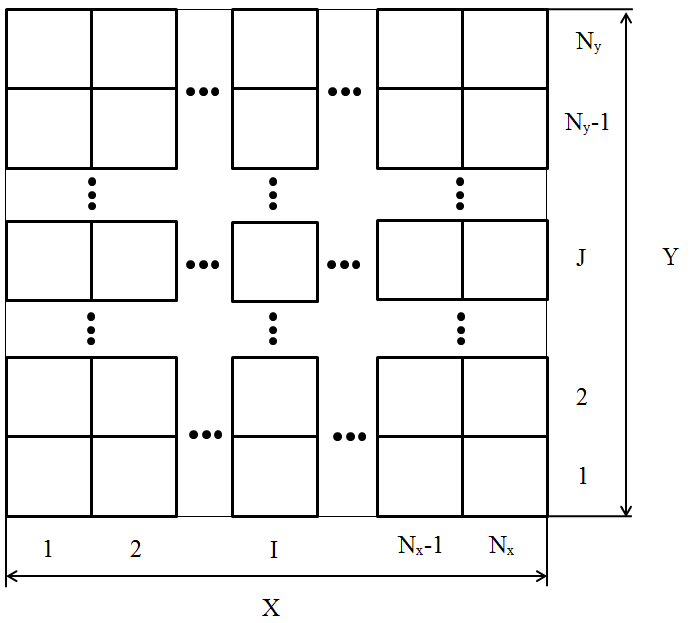
\includegraphics[width=0.60\textwidth]{figures/sec_DSA/fourier_sq_layout.png}
\caption[Fourier domain]{Fourier domain for 2D quadrilateral cells or an axial slice of 3D hexahedral cells in a regular grid.}
\label{fig::DSA_fourier_grid_layout}
\end{figure}

iteration matrices here...

spectral radius = largest eigenvalue here...

For this work, all fourier analysis was performed in MATLAB. All the eigenmodes corresponding to a fourier wave number for a given iteration matrix can be easily computed with MATLAB's built-in {\em eig} function. The maximum eigenvalue is found over the wave number space by use of the Nelder-Mead simplex algorithm \cite{nelder1965simplex}. We stress that some sort of minimization algorithm must be employed because some problem configurations can have extremely narrow local maxima. These difficult to find local maxima can correspond to the global maximum which is our desired spectral radius that we wish to compute. 

We illustrate the necessity for a minimization algorithm in Figure \ref{fig::DSA_fourier_modes_showing_search_need}. We have modeled a single 2D square mesh cell with dimensions $X=1$ and $Y=1$. The total cross section, $\sigma_t$, is set to $10^{-2}$ and the scattering ratio, $c$, set to 0.9999. We use the $S4$ level-symmetric quadrature set. The left image of Figure \ref{fig::DSA_fourier_modes_showing_search_need} has the 2D fourier wave number span the full domain space of $[\lambda_x,\lambda_y]=[0,2 \pi]^2$. The right image zooms in on the wave number ranging: $[\lambda_x,\lambda_y]=[0,1/4]^2$. From the right image, we can see two extremely narrow local maxima. We can qualitatively ascertain that these local maxima would be difficult to find if we had simply laid a grid of wave number points over $[0,2 \pi]^2$. Chang and Adams presented an even more extreme example of a difficult to find global maximum using transport synthetic acceleration \cite{chang2003analysis}.

\begin{figure}
\centering
	\begin{subfigure}[b]{0.48\textwidth}
		\centering
		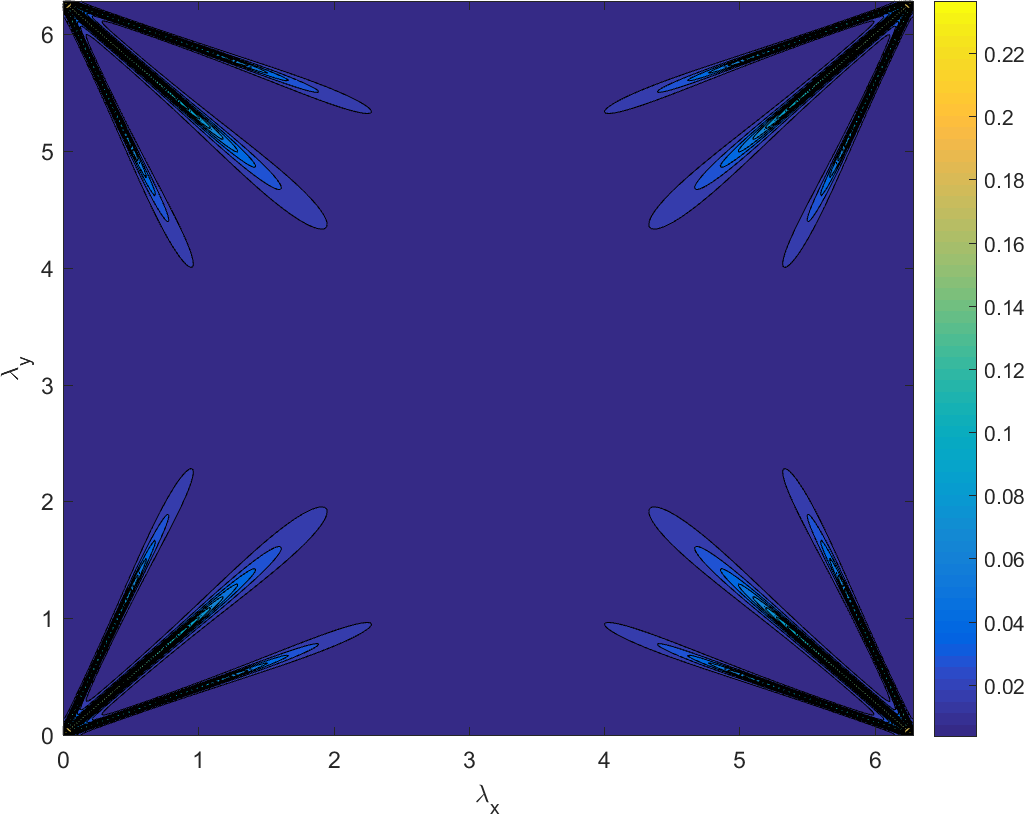
\includegraphics[width=\textwidth]{figures/sec_DSA/SI_MIP_C=4_UPWLD1_LS4_x=1e-2_dydx=1_contour.png}
		\caption{}
	\end{subfigure}
	\hfill
	\begin{subfigure}[b]{0.495\textwidth}
		\centering
		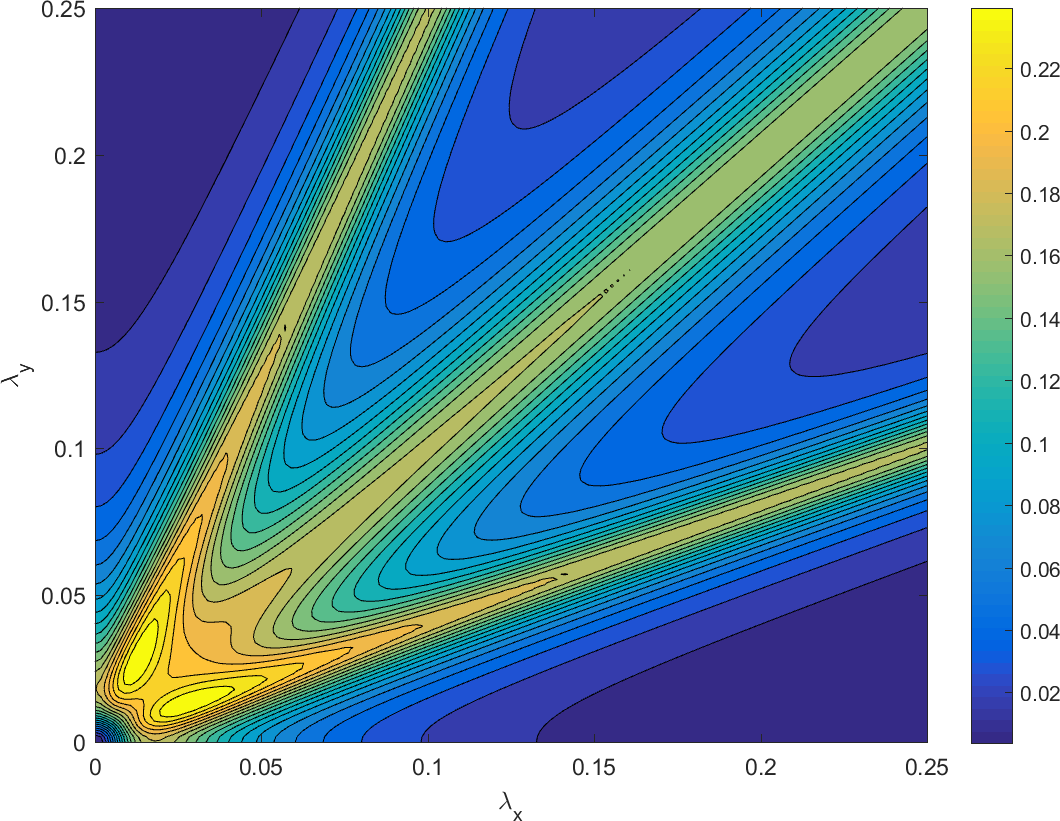
\includegraphics[width=\textwidth]{figures/sec_DSA/SI_MIP_C=4_UPWLD1_LS4_x=1e-2_dydx=1_contour_ZOOM.png}
		\caption{}
	\end{subfigure}
\caption[2D fourier wave form for MIP with the PWL coordinates]{2D fourier wave form for MIP, with 1 square cell with 1e-2 mfp, with the PWL coordinates, with the LS4 quadrature, and where the wave numbers range from: (a) $[\lambda_x,\lambda_y]=[0,2 \pi]^2$ and (b) $[\lambda_x,\lambda_y]=[0,1/4]^2$.}
\label{fig::DSA_fourier_modes_showing_search_need}
\end{figure}

%%%%%%%%%%%%%%%%%%%%%%%%%%%%%%%%%%%%%%%%%%%%%%%%%%%
%%%%%%%%%%%%%%%%%%%%%%%%%%%%%%%%%%%%%%%%%%%%%%%%%%%
%%%   Section - Results
%%%%%%%%%%%%%%%%%%%%%%%%%%%%%%%%%%%%%%%%%%%%%%%%%%%
%%%%%%%%%%%%%%%%%%%%%%%%%%%%%%%%%%%%%%%%%%%%%%%%%%%
\section{Numerical Results}
\label{sec::DSA_Results}

We now present all results 

%%%%%%%%%%%%%%%%%%%%%%%%%%%%%%%%%%%%%%%%%%%%%%%%%%%
%%%%%%%%%%%%%%%%%%%%%%%%%%%%%%%%%%%%%%%%%%%%%%%%%%%
%%%   SubSection - Thick Diffusive Limit
\subsection{Transport Solutions in the Thick Diffusive Limit}
\label{sec::DSA_Results_TDL}

We present our first numerical example by demonstrating that the various polygonal finite element basis sets satisfy the thick diffusion limit. 

\begin{equation}
\label{eq::BF_Results_TDL_trans_eq}
\vec{\Omega} \cdot \vec{\nabla} \Psi + \sigma_t \Psi =   \frac{\sigma_s}{4 \pi} \sigma_t +  \frac{Q_0}{4 \pi}
\end{equation}

\noindent As the transport problem becomes more optically thick, the total mean free paths of the neutroncs increases. In the thick diffusion limit, the domain mean free path approaches infinity. If we fix the physical dimensions of the problem to some finite value, then we can scale the cross sections and the source term to reflect the properties of the thick diffusion limit. In the limit the total and scattering cross sections tend to infinity whilc the absorption cross section and the source term tend to zero. If we introduce a scaling parameter, $\epsilon$, 

\begin{equation}
\label{eq::BF_Results_TDL_scaling}
\begin{aligned}
	\sigma_t &\rightarrow \frac{\sigma_t}{\epsilon} \\
	\sigma_a &\rightarrow \epsilon \sigma_t\\
	\sigma_s &\rightarrow \left( \frac{1}{\epsilon} - \epsilon   \right) \sigma_t \\
	\frac{Q_0}{4 \pi} &\rightarrow \epsilon \frac{Q_0}{4 \pi}
\end{aligned}
\end{equation}

\noindent Inserting these scaled cross sections and source term into Eq. (\ref{eq::BF_Results_TDL_trans_eq}) leads to following scaled transport equation:

\begin{equation}
\label{eq::BF_Results_TDL_scaled_trans_eq}
\vec{\Omega} \cdot \vec{\nabla} \Psi + \frac{\sigma_t}{\epsilon} \Psi = \sigma_t \left( \frac{1}{\epsilon} - \epsilon   \right)  \frac{\Phi}{4 \pi} + \epsilon \frac{Q_0}{4 \pi} .
\end{equation}

\noindent We can also use the scaled terms of Eq. (\ref{eq::BF_Results_TDL_scaling}) to give the corresponding scaled diffusion equation. If we take the 0th and 1st moments of Eq. (\ref{eq::BF_Results_TDL_scaled_trans_eq}) in the usual way and assume that the P1 terms obey Fick's Law, then the scaled diffusion equation is

\begin{equation}
\label{eq::BF_Results_TDL_scaled_diff_eq}
\epsilon \vec{\nabla} \cdot \frac{1}{3 \sigma_t}  \vec{\nabla} \Phi + \epsilon \sigma_t \Phi =  \epsilon Q_0.
\end{equation}

\noindent One can immediately see that Eq. (\ref{eq::BF_Results_TDL_scaled_diff_eq}) does not truly scale because there is an $\epsilon$ for each term. This is the desired behavior we want to see from the diffusion equation because, as $\epsilon \rightarrow 0$, the transport equation will converge to its diffusive limit and satisfy a diffusion equation.

For the sake of analysis, we seek to 

\begin{equation}
\label{eq::BF_Results_TDL_normalized_trans_eq}
\vec{\Omega} \cdot \vec{\nabla} \Psi + \frac{1}{\epsilon} \Psi =  \left( \frac{1}{\epsilon} - \epsilon   \right)  \frac{\Phi}{4 \pi} +  \frac{\epsilon}{4 \pi} ,
\end{equation}

\noindent and

\begin{equation}
\label{eq::BF_Results_TDL_normalized_diff_eq}
\frac{\epsilon}{3} {\nabla}^2 \Phi + \epsilon  \Phi =  \epsilon ,
\end{equation}

\noindent respectively.

%%%%%%%%%%%%%%%%%%%%%%%%%%%%%%%%%%%%%%%%%%%%%%%%%%%
%%%   SubSection - SIP Results
\subsection{SIP used as a Diffusion Solver}
\label{sec::DSA_Results_SIP}

We first wish to know how an interior penalty form of the diffusion equation will perform on unstructured polyhedral grids. The SIP diffusion formulation has previously been analyzed for use as a DFEM diffusion solver for unstructured 2D polygonal grids \cite{ragusa2015discontinuous}. The MIP DSA form has also been successfully utilized for unstructured 2D polygonal grids \cite{turcksin2014discontinuous}. Here, we first seek to extend the efficacy of the SIP form as a diffusion solver on polyhedral mesh cellls. We will do this by analyzing the following two problem types:

\begin{enumerate}
	\item An exactly-linear solution to determine if linear basis functions will span the solution space;
	\item The Method of Manufactured Solutions (MMS) to test basis function convergence rates.
\end{enumerate}

The polyhedral mesh types that we employ for this analysis are presented in Section \ref{sec::DSA_Results_SIP_Geometry}. Next, the exactly-linear solution analysis is performed in Section \ref{sec::DSA_Results_SIP_Linear}. Finally, the MMS analysis to confirm the second order convergence rates of the 3D PWL basis functions is presented in Section \ref{sec::DSA_Results_SIP_MMS}.

%%%%%%%%%%%%%%%%%%%%%%%%%%%%%%%%%%%%%%%%%%%%%%%%%%%
%%%   SubSubSection - SIP Results = Geometry
\subsubsection{Geometry Specification for the SIP Problems}
\label{sec::DSA_Results_SIP_Geometry}

To analyze the SIP diffusion form on 3D polyhedral grids, we will utilize many of the 2D polygonal grids that were used in Section \ref{sec::BF_Results_Linear}. For this analysis we will resuse the cartesian, ordered-triangular, polygonal sinusoidal, and polygonal-z meshes. We will also use purely-randomized polygonal grids formed from Voronoi mesh generation as outlined in Section \ref{sec::Sn_Solution_Spatial_Voronoi}. To form the needed 3D polyhedral grids, we will take these 2D grids and simply extrude the meshes in the z-dimension. 

Figure \ref{fig::SIP_mesh_slices} provides the 2D mesh types that will be utilized in this analysis. Figure \ref{fig::SIP_mesh_extruded} then provides the same meshes after they have been extruded in the z-dimension. We note that it will not simply be these exact grids that are employed. For the MMS analysis in Section \ref{sec::DSA_Results_SIP_MMS}, various refinements of these meshes will be utilized.

\begin{figure}
\centering
	\begin{subfigure}[b]{0.5\textwidth}
		\centering
		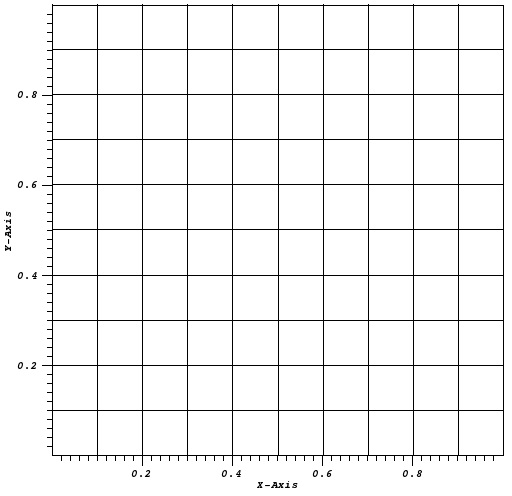
\includegraphics[width=0.82\textwidth]{figures/sec_DSA/SIP_cart_mesh.png}
		\caption{}
	\end{subfigure}
	\vfill
	\begin{subfigure}[b]{0.45\textwidth}
		\centering
		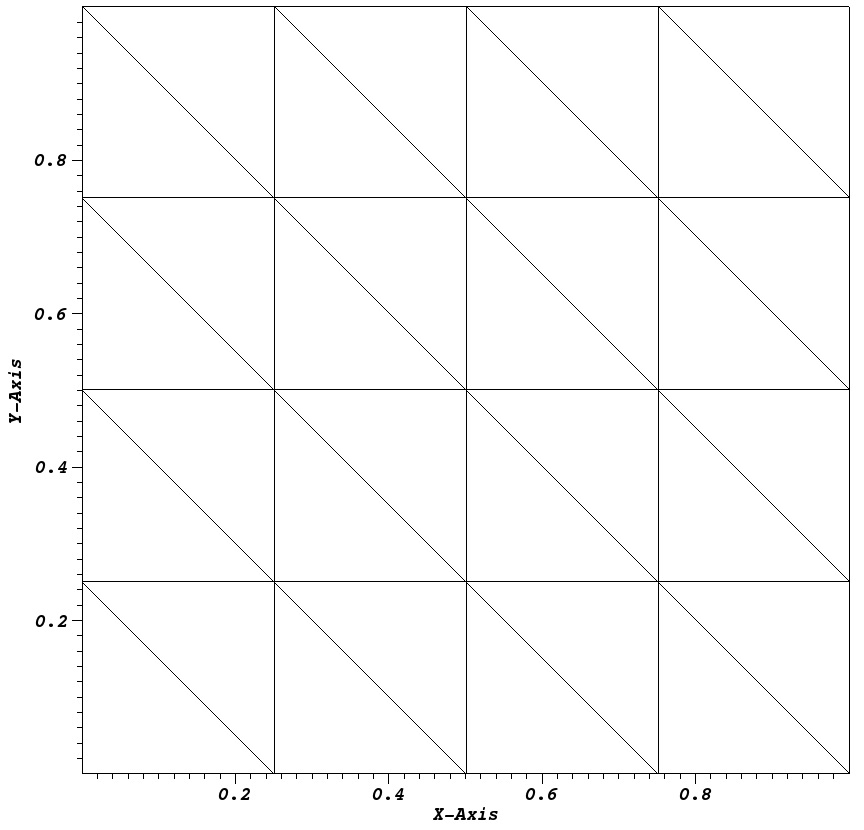
\includegraphics[width=0.85\textwidth]{figures/sec_DSA/SIP_tri_mesh.png}
		\caption{}
	\end{subfigure}
	\hfill
	\begin{subfigure}[b]{0.45\textwidth}
		\centering
		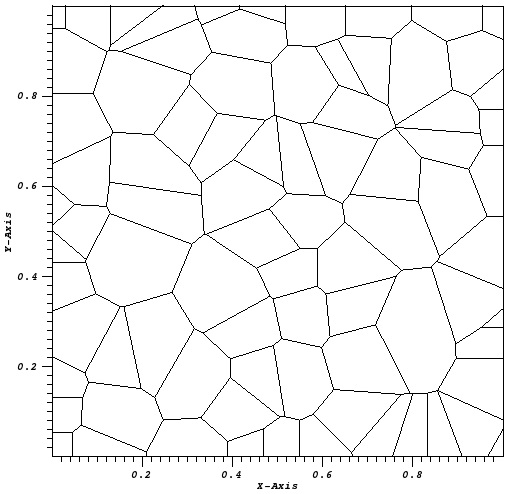
\includegraphics[width=0.85\textwidth]{figures/sec_DSA/SIP_poly_mesh.png}
		\caption{}
	\end{subfigure}
	\vfill
	\begin{subfigure}[b]{0.45\textwidth}
		\centering
		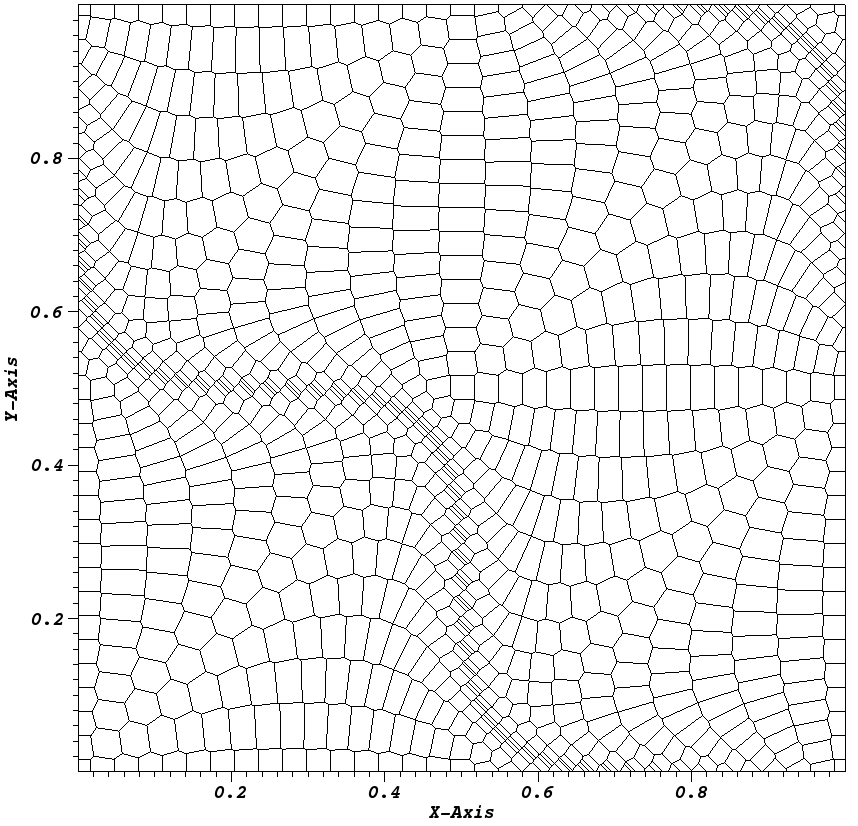
\includegraphics[width=0.85\textwidth]{figures/sec_DSA/SIP_sine_poly_mesh.png}
		\caption{}
	\end{subfigure}
	\hfill
	\begin{subfigure}[b]{0.45\textwidth}
		\centering
		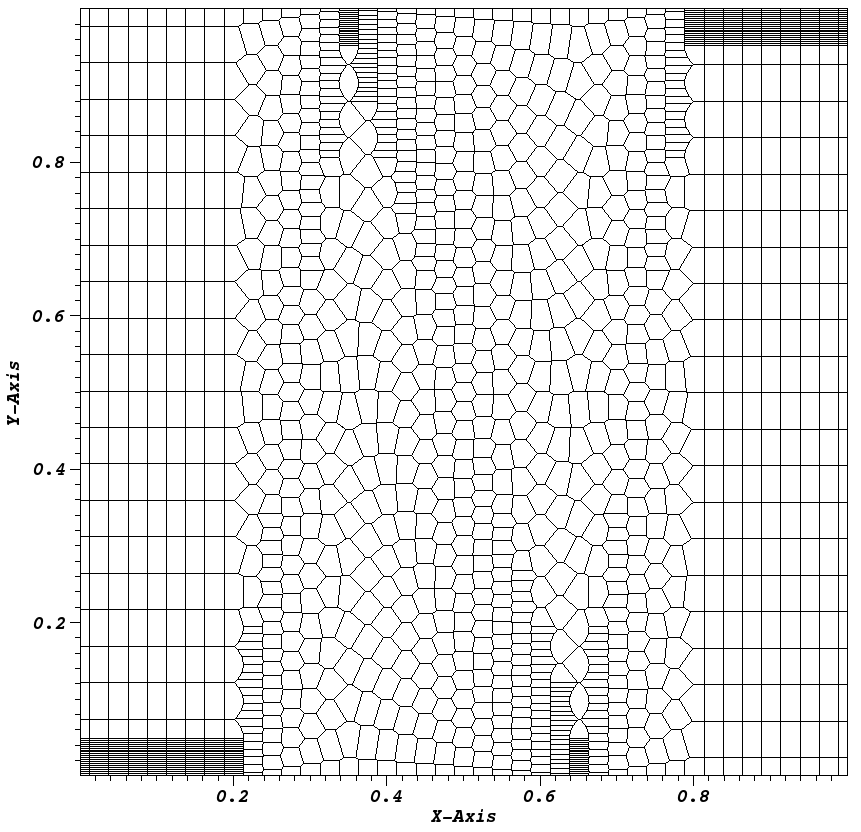
\includegraphics[width=0.85\textwidth]{figures/sec_DSA/SIP_z_poly_mesh.png}
		\caption{}
	\end{subfigure}
\caption{2D grids to be extruded of the different mesh types: (a) cartesian, (b) ordered triangles, (c) random polygons, (d) sinusoidal polygons, and (e) polygonal z-mesh.}
\label{fig::SIP_mesh_slices}
\end{figure}

\begin{figure}
\centering
	\begin{subfigure}[b]{0.5\textwidth}
		\centering
		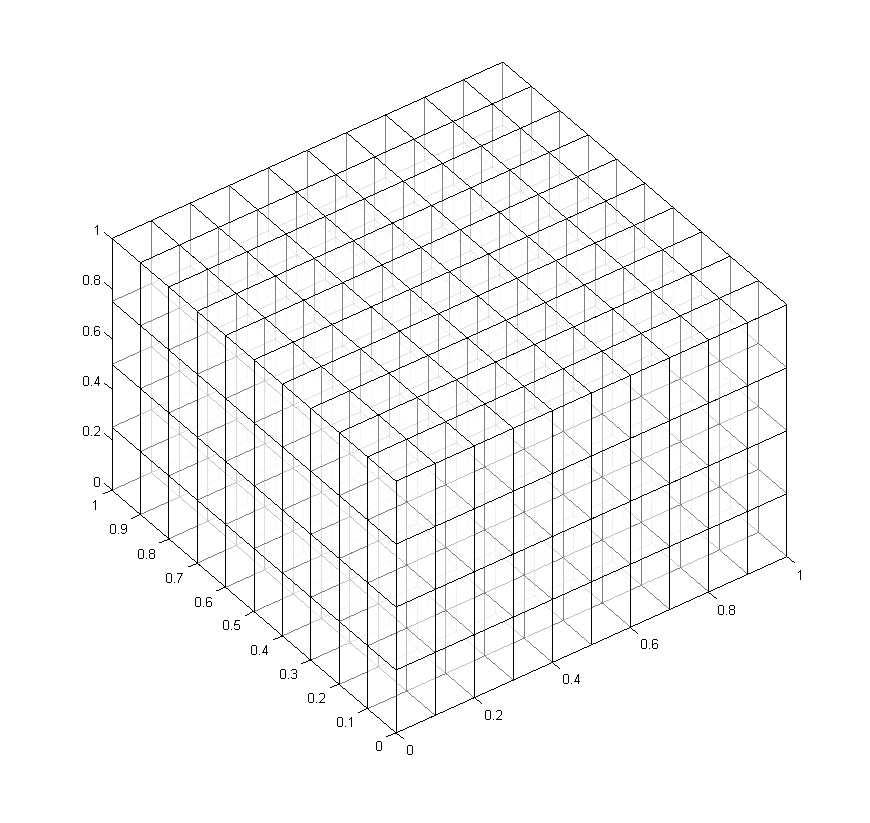
\includegraphics[width=0.82\textwidth]{figures/sec_DSA/SIP_cart_extruded_mesh.png}
		\caption{}
	\end{subfigure}
	\vfill
	\begin{subfigure}[b]{0.45\textwidth}
		\centering
		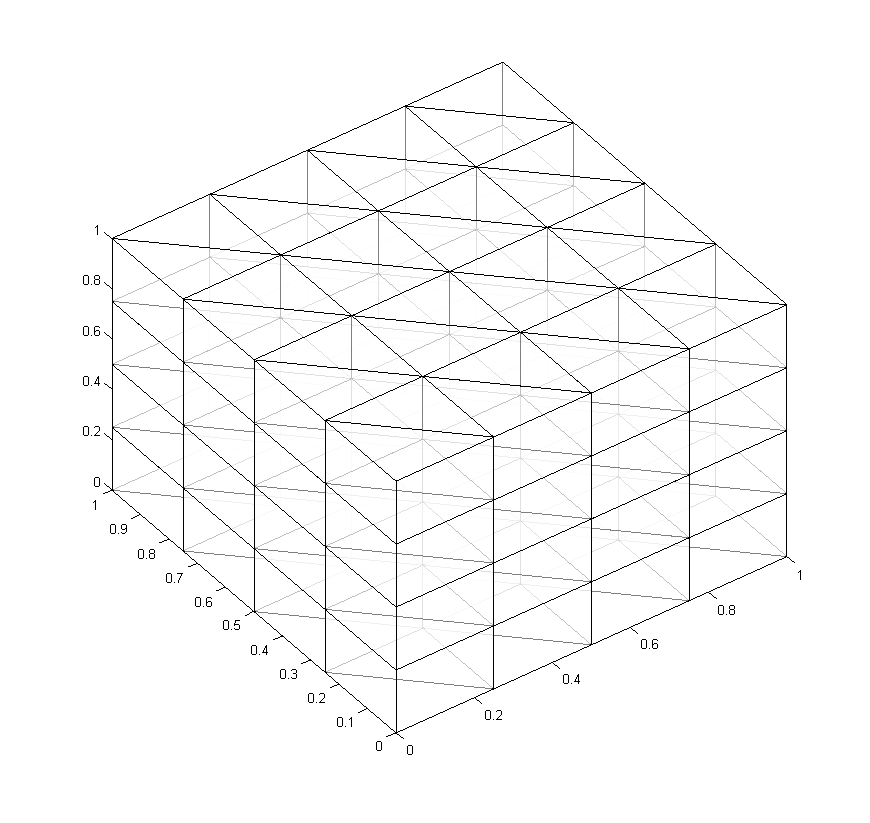
\includegraphics[width=0.85\textwidth]{figures/sec_DSA/SIP_tri_extruded_mesh.png}
		\caption{}
	\end{subfigure}
	\hfill
	\begin{subfigure}[b]{0.45\textwidth}
		\centering
		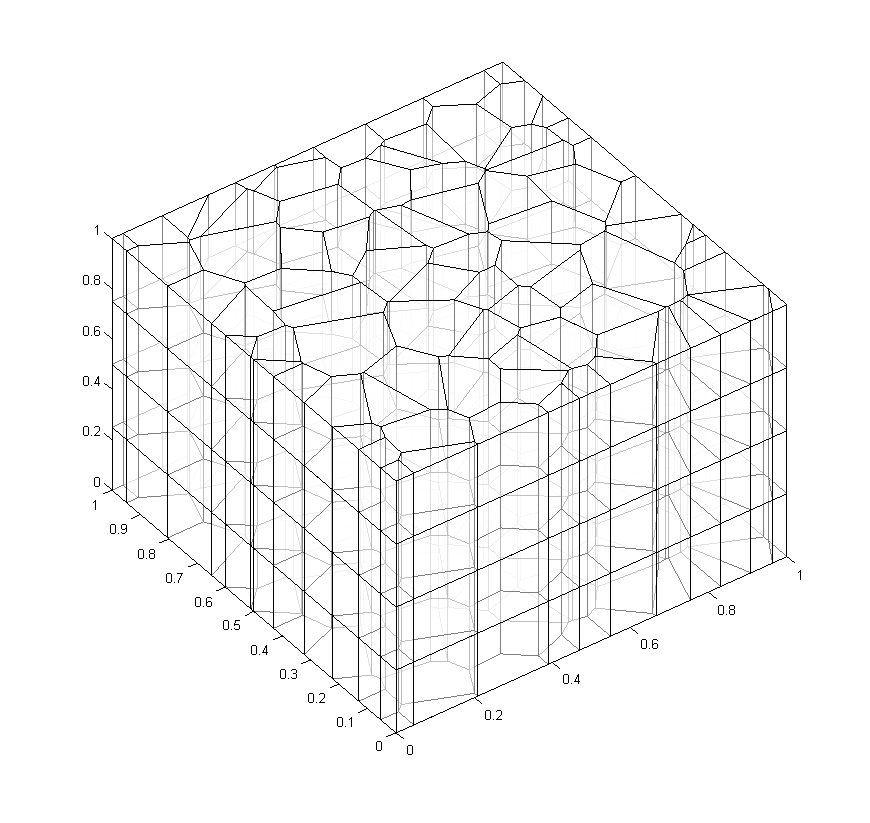
\includegraphics[width=0.85\textwidth]{figures/sec_DSA/SIP_poly_extruded_mesh.png}
		\caption{}
	\end{subfigure}
	\vfill
	\begin{subfigure}[b]{0.45\textwidth}
		\centering
		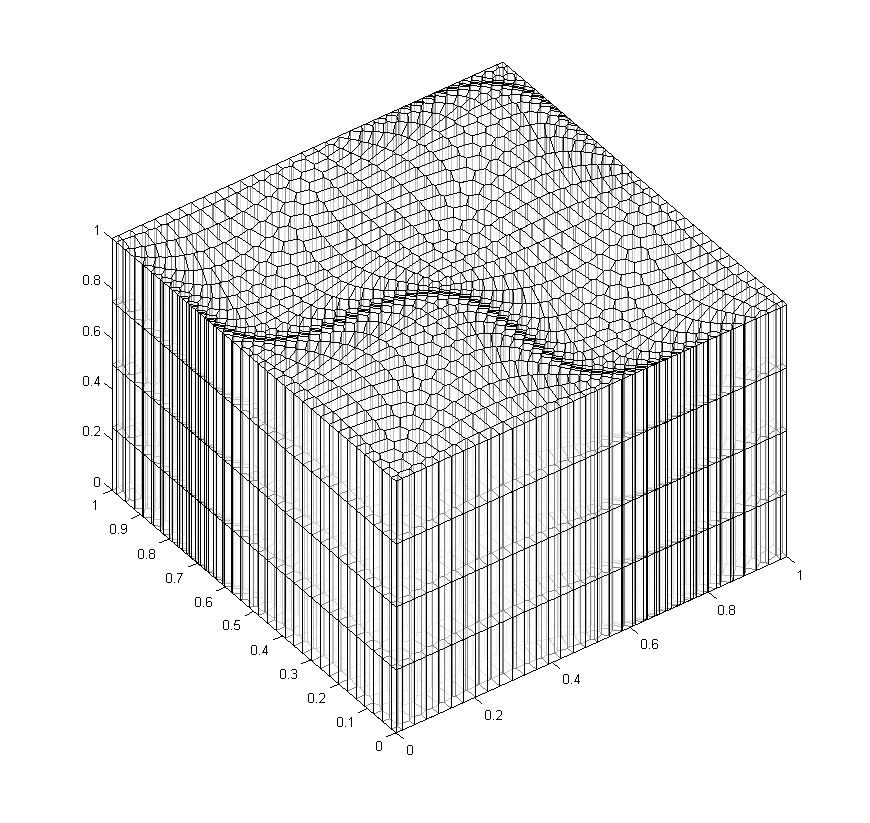
\includegraphics[width=0.85\textwidth]{figures/sec_DSA/SIP_sine_poly_extruded_mesh.png}
		\caption{}
	\end{subfigure}
	\hfill
	\begin{subfigure}[b]{0.45\textwidth}
		\centering
		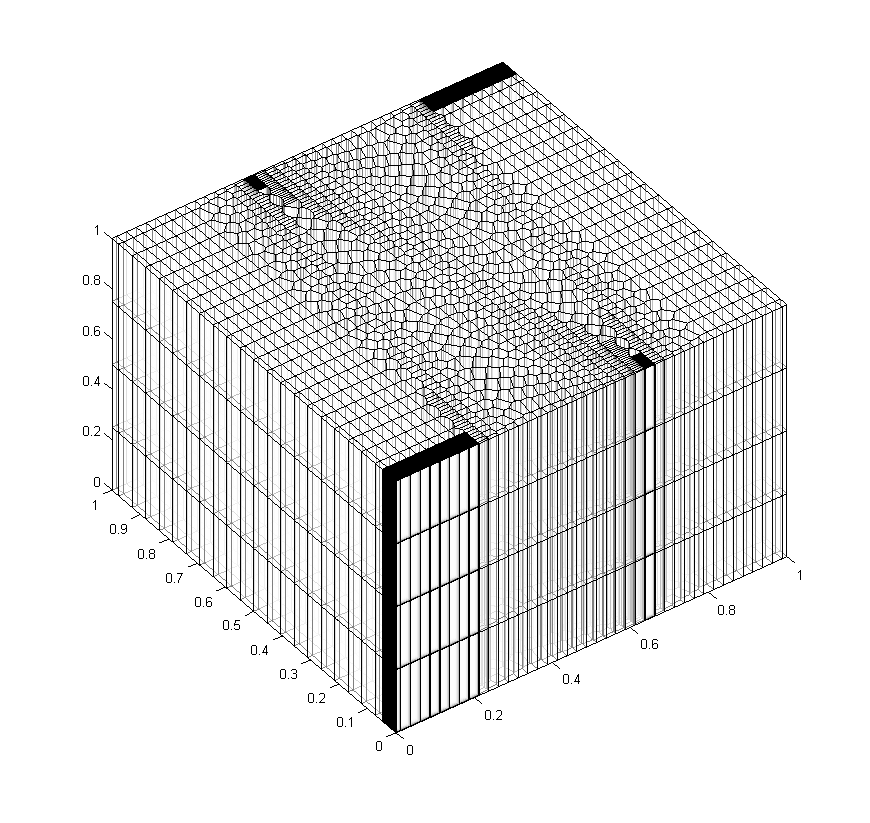
\includegraphics[width=0.85\textwidth]{figures/sec_DSA/SIP_z_poly_extruded_mesh.png}
		\caption{}
	\end{subfigure}
\caption{Extrusion of the different mesh types: (a) cartesian, (b) ordered triangles, (c) random polygons, (d) sinusoidal polygons, and (e) polygonal z-mesh.}
\label{fig::SIP_mesh_extruded}
\end{figure}

%%%%%%%%%%%%%%%%%%%%%%%%%%%%%%%%%%%%%%%%%%%%%%%%%%%
%%%   SubSubSection - SIP Results = Linear
\subsubsection{Exactly-Linear Solution}
\label{sec::DSA_Results_SIP_Linear}

We first test SIP by enforcing a sytem that yields an exactly-linear diffusion solution. Linear finite elements should then theoretically fully-span the solution space. We can achieve this mathematically by setting the cross-section and right-hand-source terms to zero, $\sigma = Q = 0$. Robin boundary conditions are imposed on opposite faces in 1 dimension, with homogeneous Neumann boundary conditions on all other faces. If the Robin boundaries are chosen in the y-direction, with $y \in (0,L)$, then the analytical solution for the problem will be 

\begin{equation}
\label{eq::SIP_mms_lin_solution}
\Phi(x,y,z) = \frac{4 J^{inc}}{L + 4D} \left(  L + 2 D - y \right),
\end{equation}

\noindent with the following boundary conditions in the y-direction:

\begin{equation}
\label{eq::SIP_mms_lin_bcs}
\begin{aligned}
\Phi - 2D \partial_y \Phi = & 4 J^{inc}, \qquad & \forall (x,z),y=0 \\
\Phi + 2D \partial_y \Phi = & 0, \qquad & \forall (x,z),y=L
\end{aligned}.
\end{equation}

\noindent In Eqs. (\ref{eq::SIP_mms_lin_solution}) and (\ref{eq::SIP_mms_lin_bcs}), $D$ is once again the standard diffusion coefficient and $J^{inc}$ is the incoming current on the $y=0$ boundary. For this analysis, we choose $D$ to be 2, $J^{inc}$ to be 9, and $L$ to be 1. Using Eq. (\ref{eq::SIP_mms_lin_solution}), our solution has a value of 20 at $y=0$ and linearly-decreases to 16 at $y=1$.

Using the 3D PWL basis functions, which were previously used for SIP on 2D polygons \cite{ragusa2015discontinuous}, the linear solutions are presented in Figure \ref{fig::SIP_linear_sol} at the midplane axial slice of $z=L/2$. We can see from the exact contour lines in the plots that SIP can capture an exactly-linear solution even on some highly distorted polyhedral grids.

\begin{figure}
\centering
	\begin{subfigure}[b]{0.5\textwidth}
		\centering
		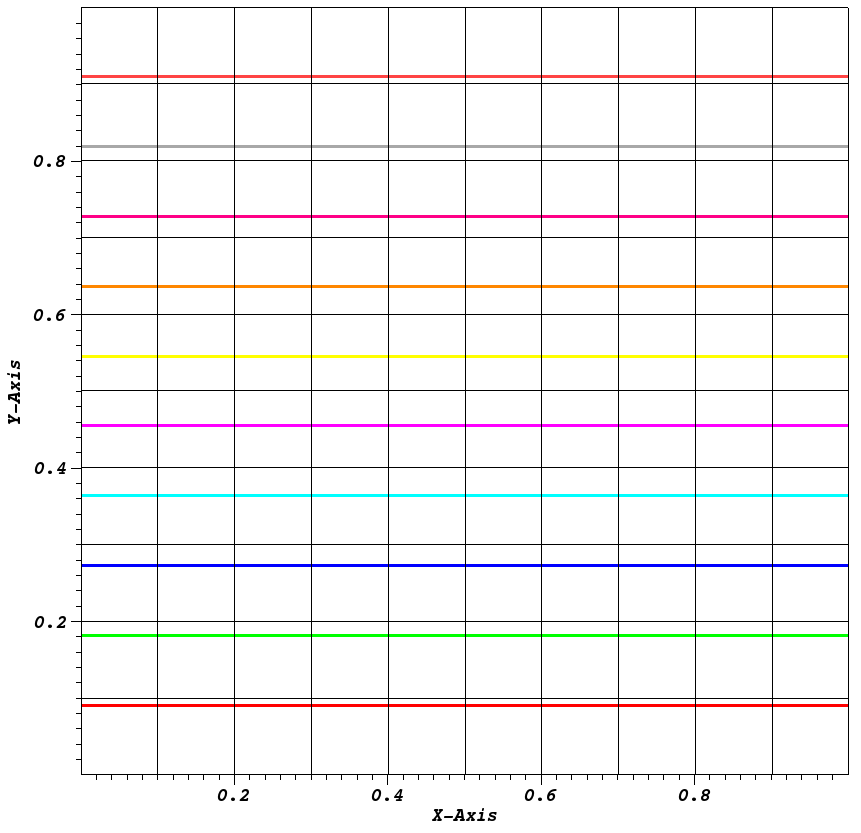
\includegraphics[width=0.82\textwidth]{figures/sec_DSA/SIP_cart_lin_contour.png}
		\caption{}
	\end{subfigure}
	\vfill
	\begin{subfigure}[b]{0.45\textwidth}
		\centering
		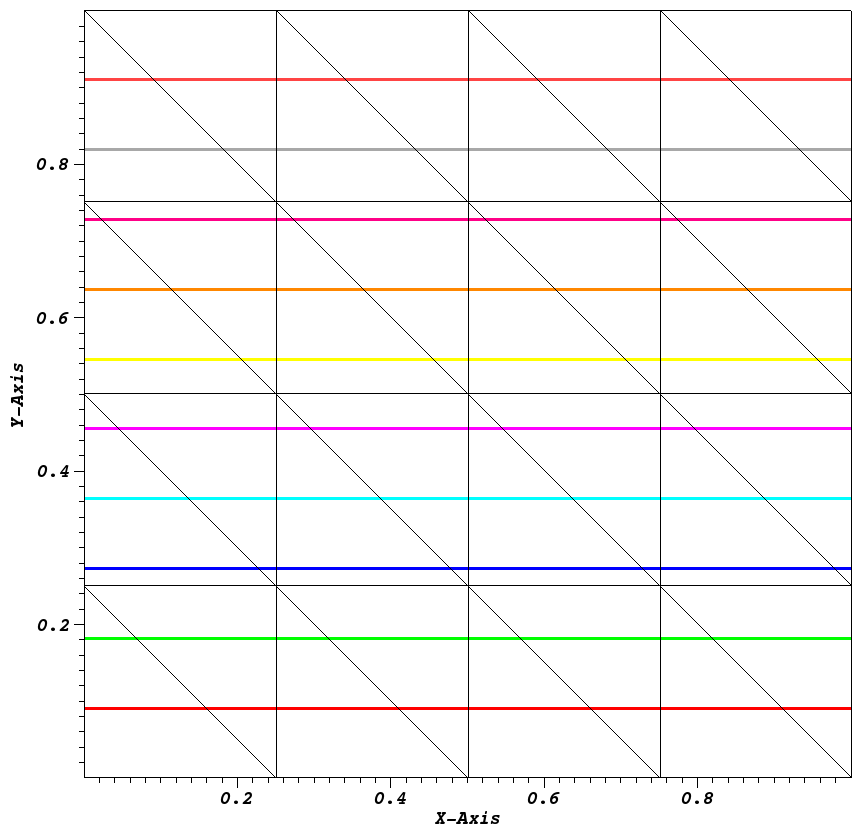
\includegraphics[width=0.85\textwidth]{figures/sec_DSA/SIP_tri_lin_contour.png}
		\caption{}
	\end{subfigure}
	\hfill
	\begin{subfigure}[b]{0.45\textwidth}
		\centering
		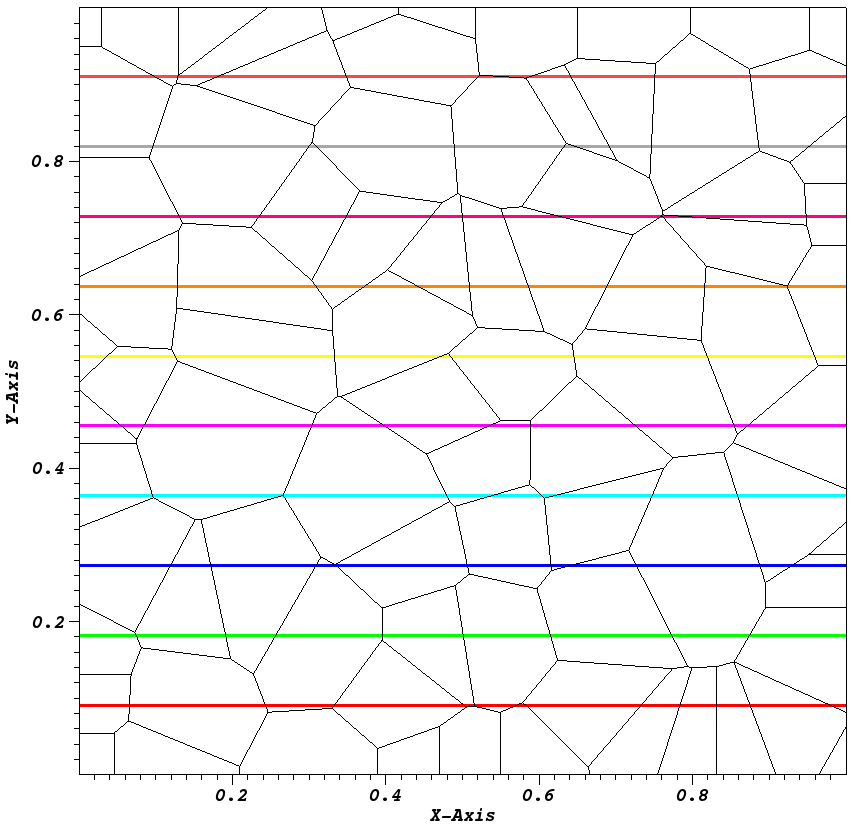
\includegraphics[width=0.85\textwidth]{figures/sec_DSA/SIP_poly_lin_contour.png}
		\caption{}
	\end{subfigure}
	\vfill
	\begin{subfigure}[b]{0.45\textwidth}
		\centering
		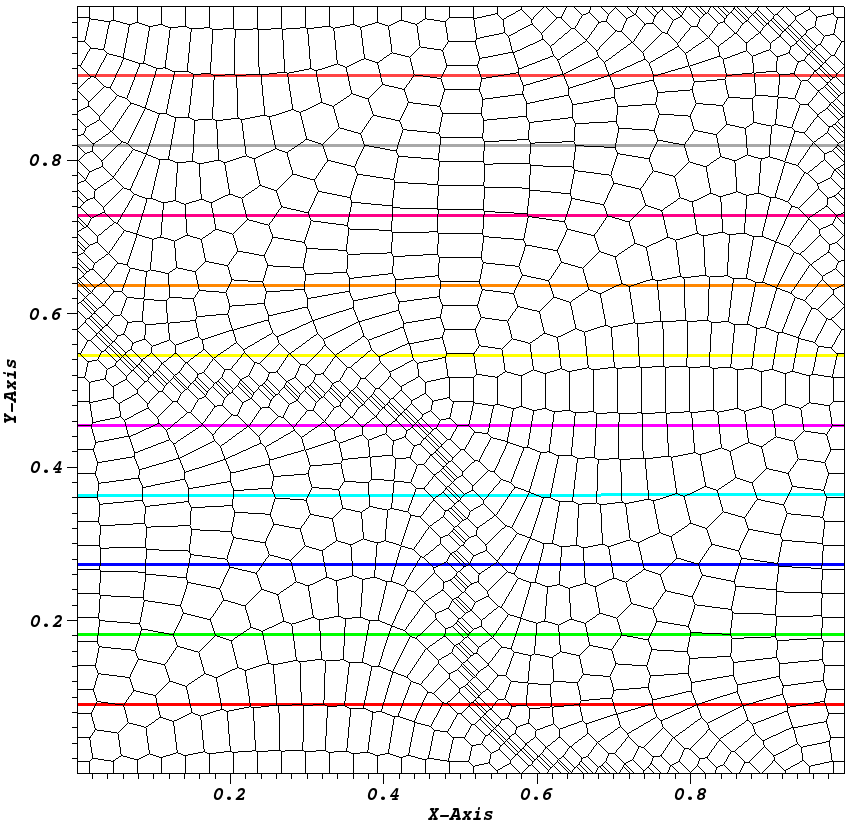
\includegraphics[width=0.85\textwidth]{figures/sec_DSA/SIP_sine_poly_lin_contour.png}
		\caption{}
	\end{subfigure}
	\hfill
	\begin{subfigure}[b]{0.45\textwidth}
		\centering
		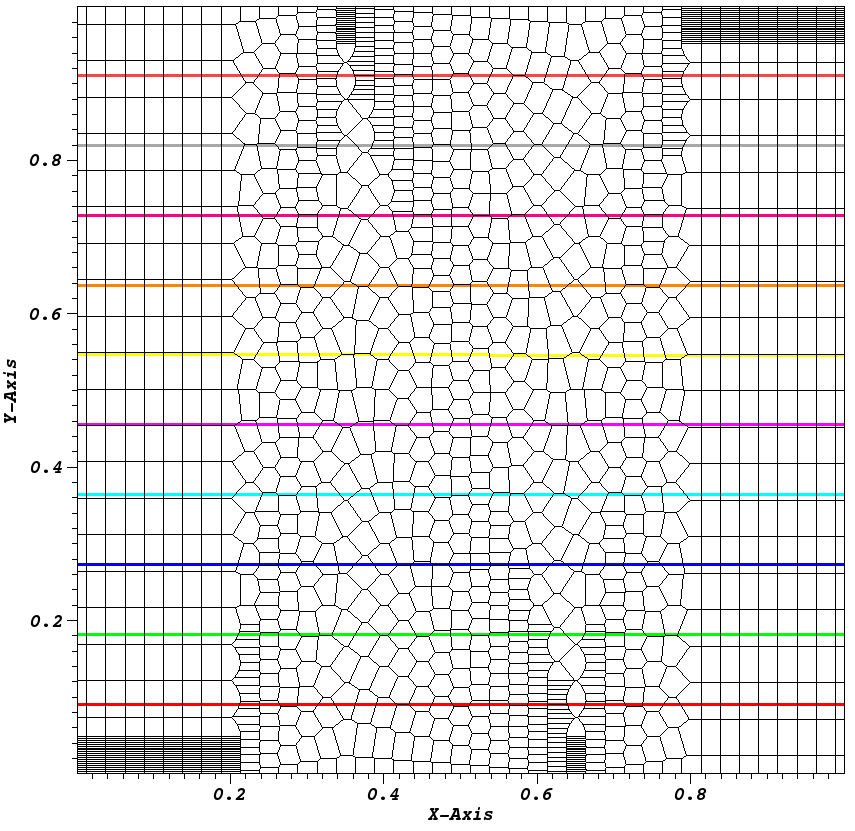
\includegraphics[width=0.85\textwidth]{figures/sec_DSA/SIP_z_poly_lin_contour.png}
		\caption{}
	\end{subfigure}
\caption{Axial slice showing the contours for the linear solution of the different mesh types: (a) cartesian, (b) ordered triangles, (c) random polygons, (d) sinusoidal polygons, and (e) polygonal z-mesh.}
\label{fig::SIP_linear_sol}
\end{figure}

%%%%%%%%%%%%%%%%%%%%%%%%%%%%%%%%%%%%%%%%%%%%%%%%%%%
%%%   SubSubSection - SIP Results = MMS
\subsubsection{Method of Manufactured Solutions}
\label{sec::DSA_Results_SIP_MMS}

We next test to see if the SIP diffusion form can capture the appropriate second order convergencerates with the 3D PWL basis functions. These basis functions were previously shown to capture the appropriate convergence rates for the DGFEM transport equation on 3D hexahedral grids \cite{bailey2008phd}.

\begin{equation}
\label{eq::SIP_quad_mms_solution}
\begin{aligned}
\Phi^{quad} (x,y,z) = x(1-x)y(1-y)z(1-z) 
\end{aligned}
\end{equation}

\begin{equation}
\label{eq::SIP_gauss_mms_solution}
\begin{aligned}
\Phi^{gauss} (x,y,z) = \Phi^{quad} (x,y,z) \exp(- (\vec{r} - \vec{r}_0) \cdot (\vec{r} - \vec{r}_0)^{T}  )
\end{aligned}
\end{equation}


\begin{figure}
\centering
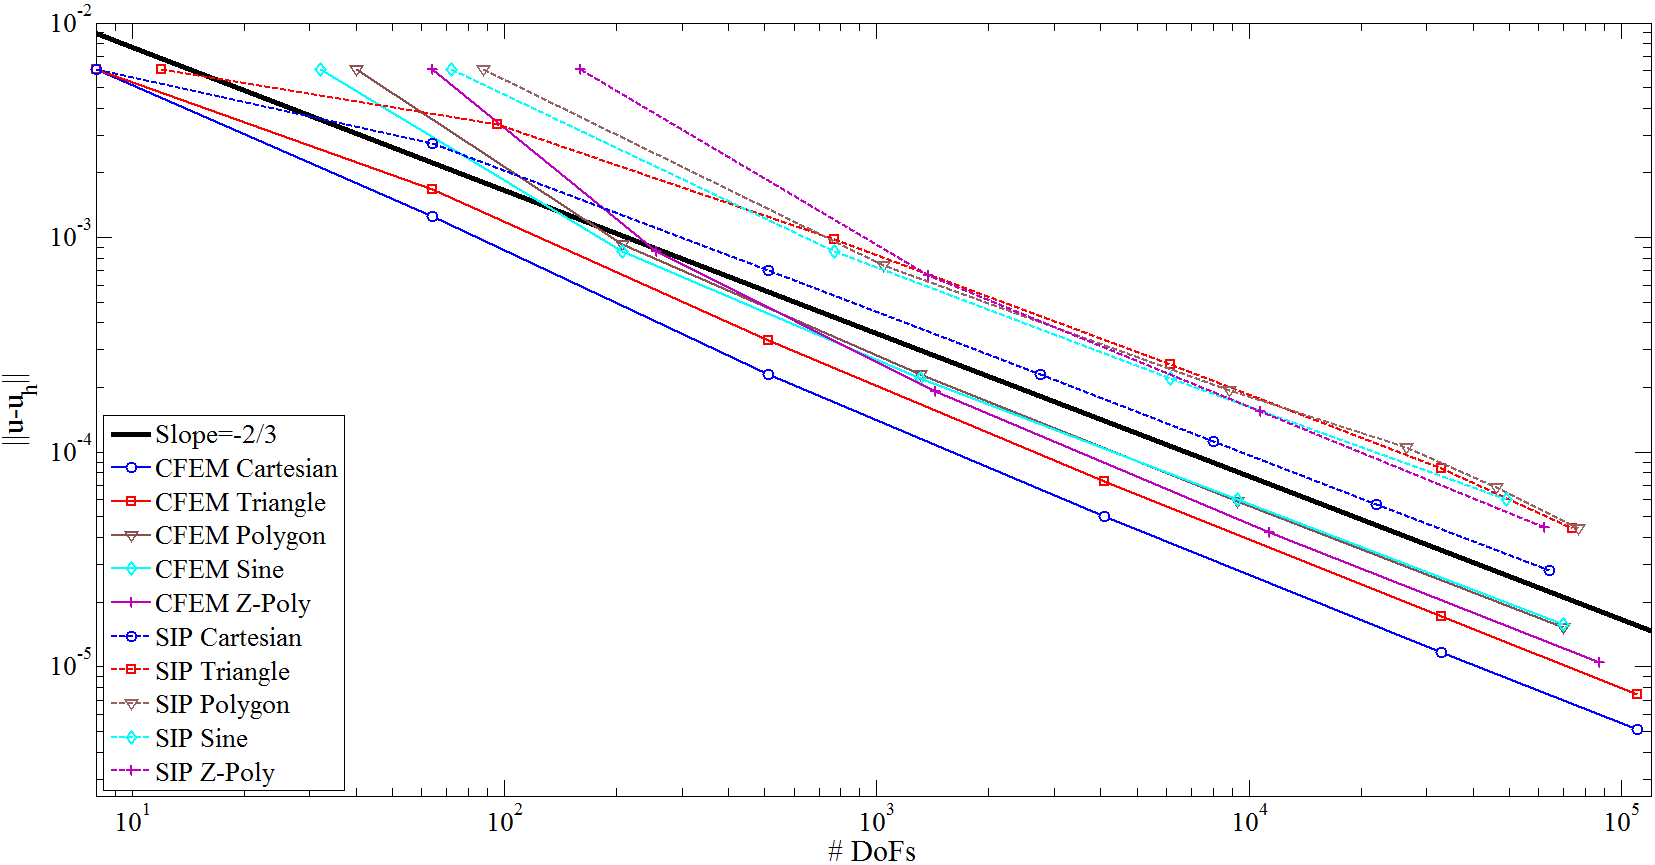
\includegraphics[width=\textwidth]{figures/sec_DSA/SIP_mms_3d_quad_full_paint.png}
\caption{blah}
\label{fig::SIP_mms_quad_error_plot}
\end{figure}

\begin{figure}
\centering
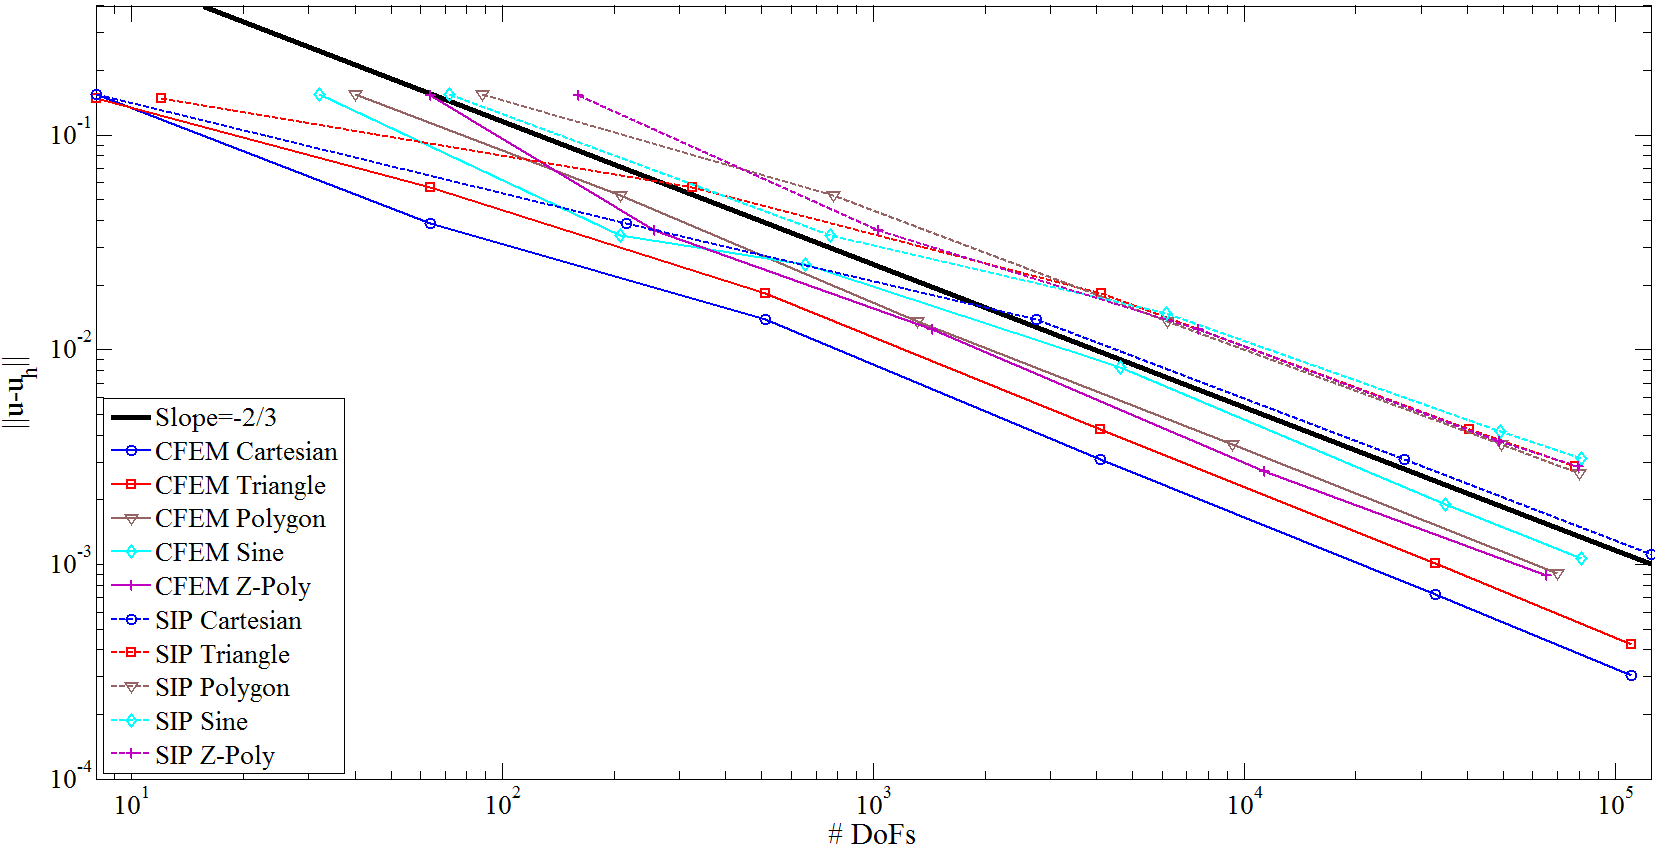
\includegraphics[width=\textwidth]{figures/sec_DSA/SIP_mms_3d_gauss_full_paint.png}
\caption{blah}
\label{fig::SIP_mms_gauss_error_plot}
\end{figure}


%%%%%%%%%%%%%%%%%%%%%%%%%%%%%%%%%%%%%%%%%%%%%%%%%%%
%%%%%%%%%%%%%%%%%%%%%%%%%%%%%%%%%%%%%%%%%%%%%%%%%%%
%%%   SubSection - 1Group Analysis
\subsection{1 Group DSA Analysis}
\label{sec::DSA_Results_1G}

%%%%%%%%%%%%%%%%%%%%%%%%%%%%%%%%%%%%%%%%%%%%%%%%%%%
%%%   SubSubSection -  2D Homogeneous Medium
\subsubsection{2D Homogeneous Medium Case}
\label{sec::DSA_Results_1G_2DHomo}

\begin{figure}
\centering
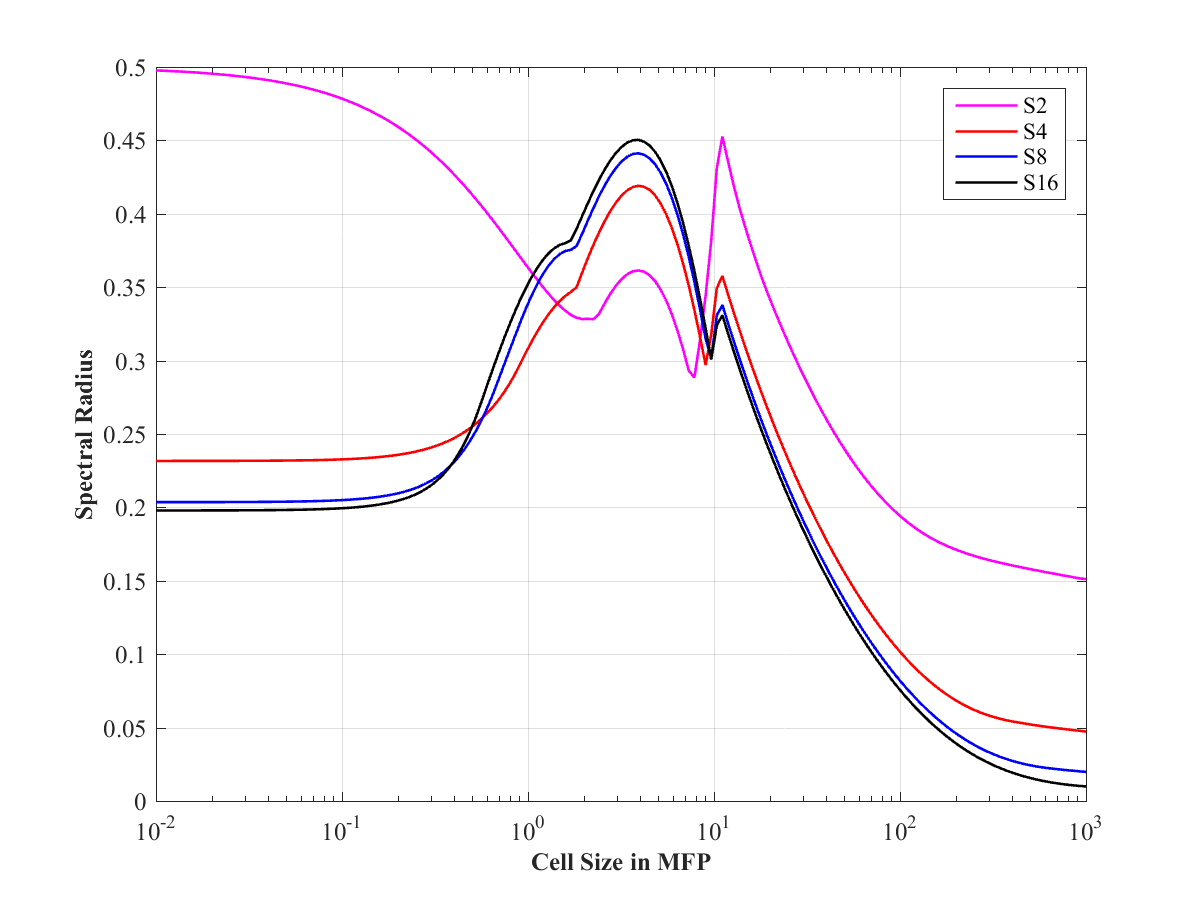
\includegraphics[width=0.75\textwidth]{figures/sec_DSA/SI_MIP_quad_C=4_Wachspress1_LS2,4,8,16.png}
\caption{Fourier analysis of the 2D MIP form with $c=4$ and using the linear Wachspress coordinates for the homogeneous infinite medium case as a function of the mesh optical thickness.}
\label{fig::DSA_1G_Fourier_Wach1}
\end{figure}

\begin{figure}
\centering
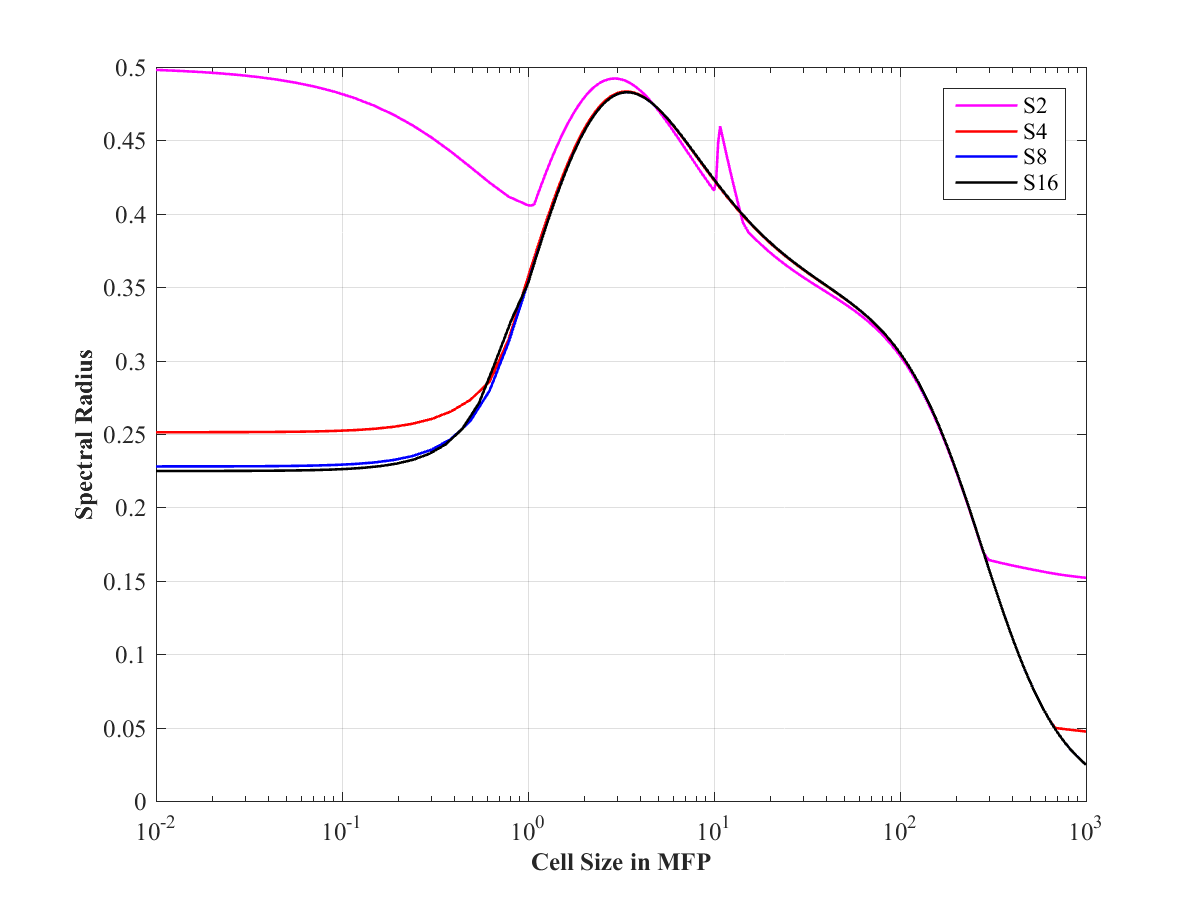
\includegraphics[width=0.75\textwidth]{figures/sec_DSA/SI_MIP_quad_C=4_PWLD1_LS2,4,8,16.png}
\caption{Fourier analysis of the 2D MIP form with $c=4$ and using the linear PWL coordinates for the homogeneous infinite medium case as a function of the mesh optical thickness.}
\label{fig::DSA_1G_Fourier_PWL1}
\end{figure}

\begin{figure}
\centering
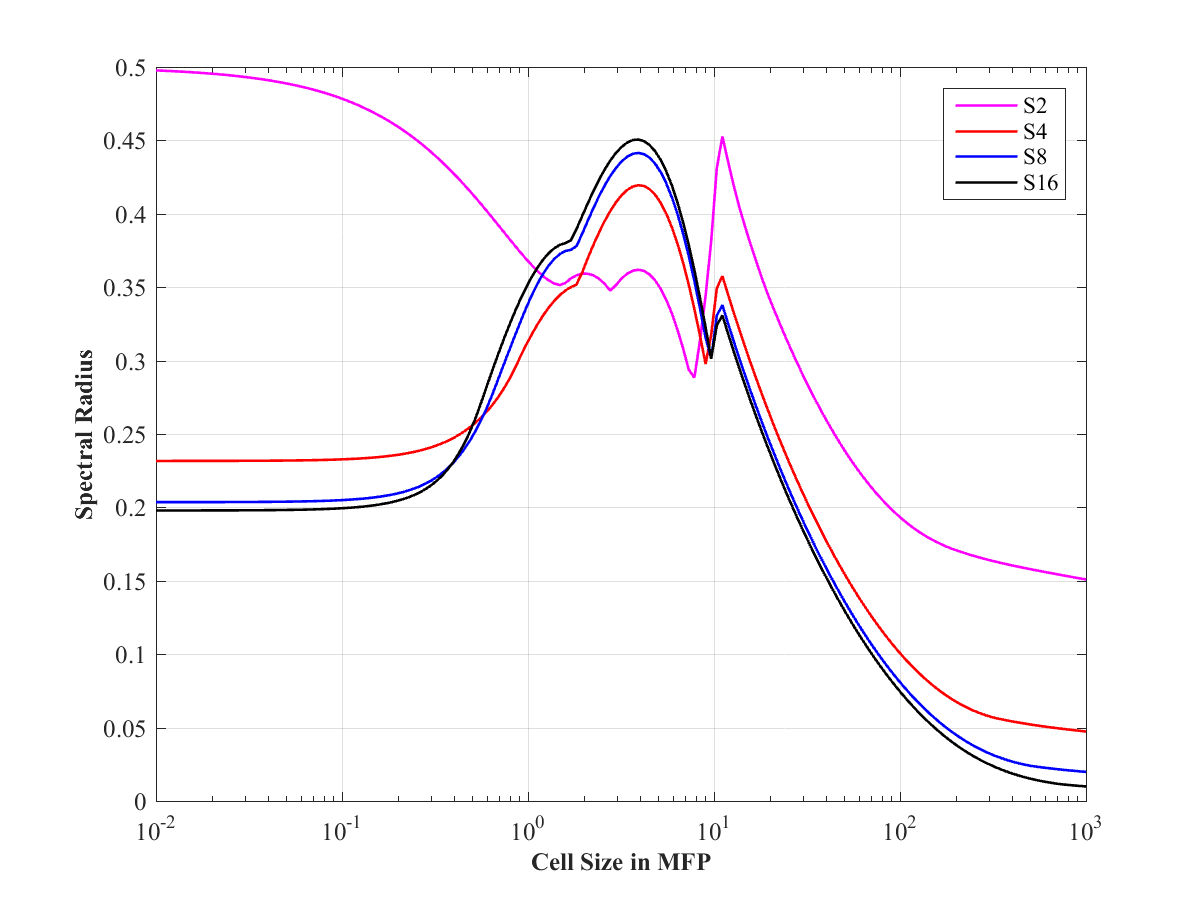
\includegraphics[width=0.75\textwidth]{figures/sec_DSA/SI_MIP_quad_C=4_MV1_LS2,4,8,16.png}
\caption{Fourier analysis of the 2D MIP form with $c=4$ and using the linear mean value coordinates for the homogeneous infinite medium case as a function of the mesh optical thickness.}
\label{fig::DSA_1G_Fourier_MV1}
\end{figure}

\begin{figure}
\centering
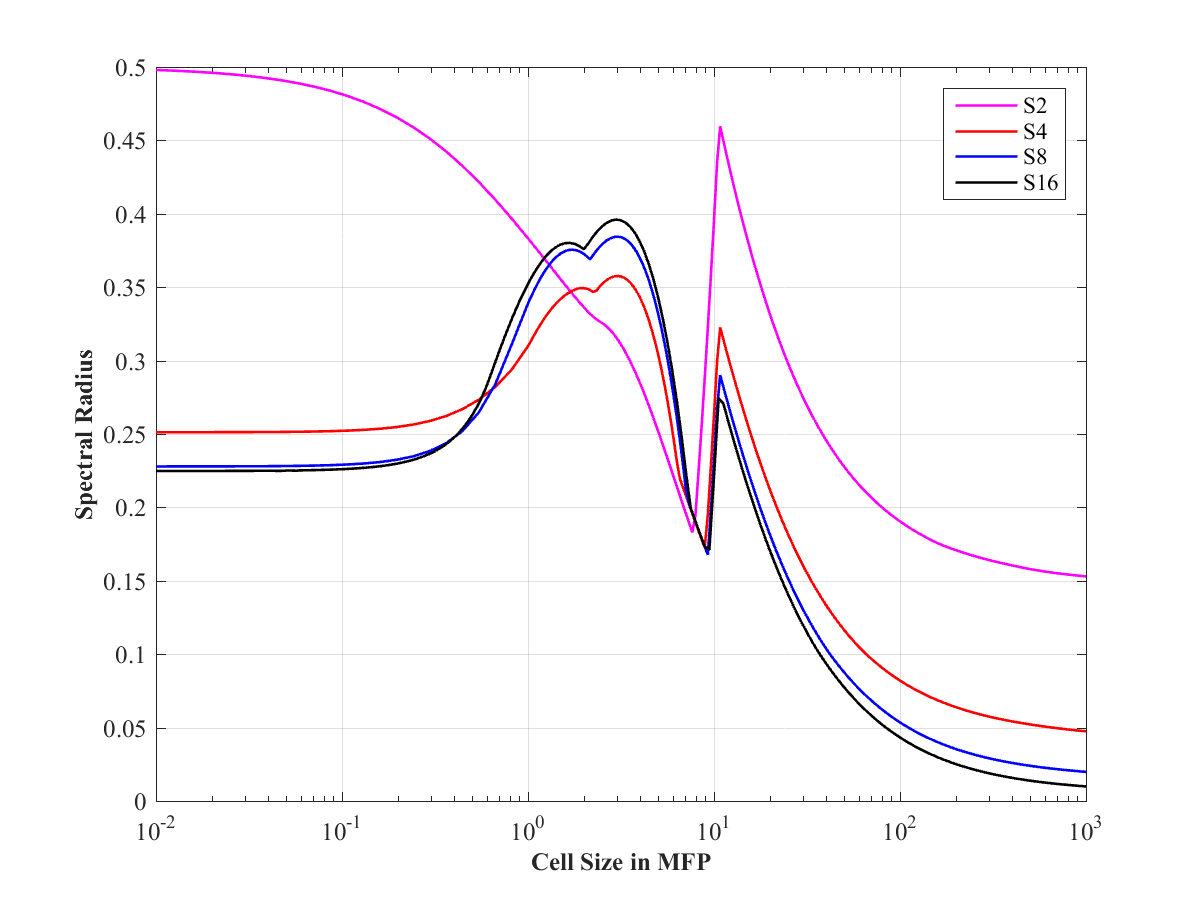
\includegraphics[width=0.75\textwidth]{figures/sec_DSA/SI_MIP_quad_C=4_MAXENT1_LS2,4,8,16.png}
\caption{Fourier analysis of the 2D MIP form with $c=4$ and using the linear maximum entropy coordinates for the homogeneous infinite medium case as a function of the mesh optical thickness.}
\label{fig::DSA_1G_Fourier_ME1}
\end{figure}

\begin{figure}
\centering
	{
	\begin{subfigure}[b]{0.485\textwidth}
		\centering
		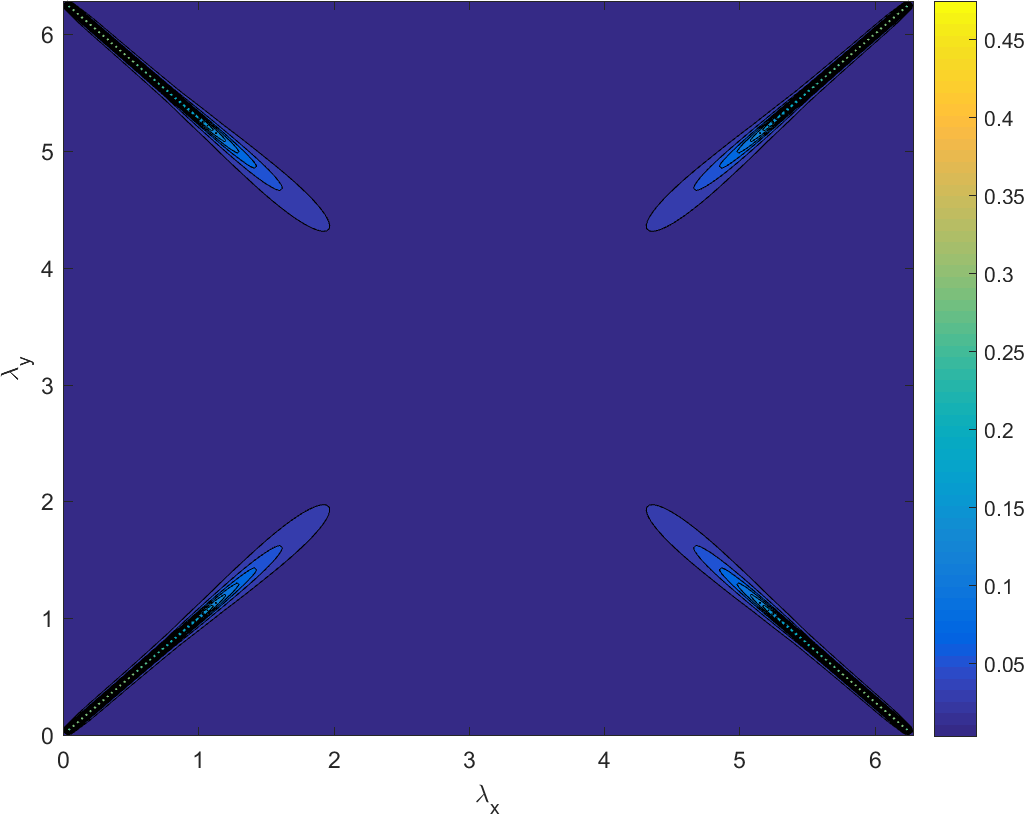
\includegraphics[width=0.975\textwidth]{figures/sec_DSA/SI_MIP_C=4_UPWLD1_LS2_x=1e-2_dydx=1_contour.png}
		\caption{$10^{-2}$ mfp}
	\end{subfigure}
	\hfill
	\begin{subfigure}[b]{0.485\textwidth}
		\centering
		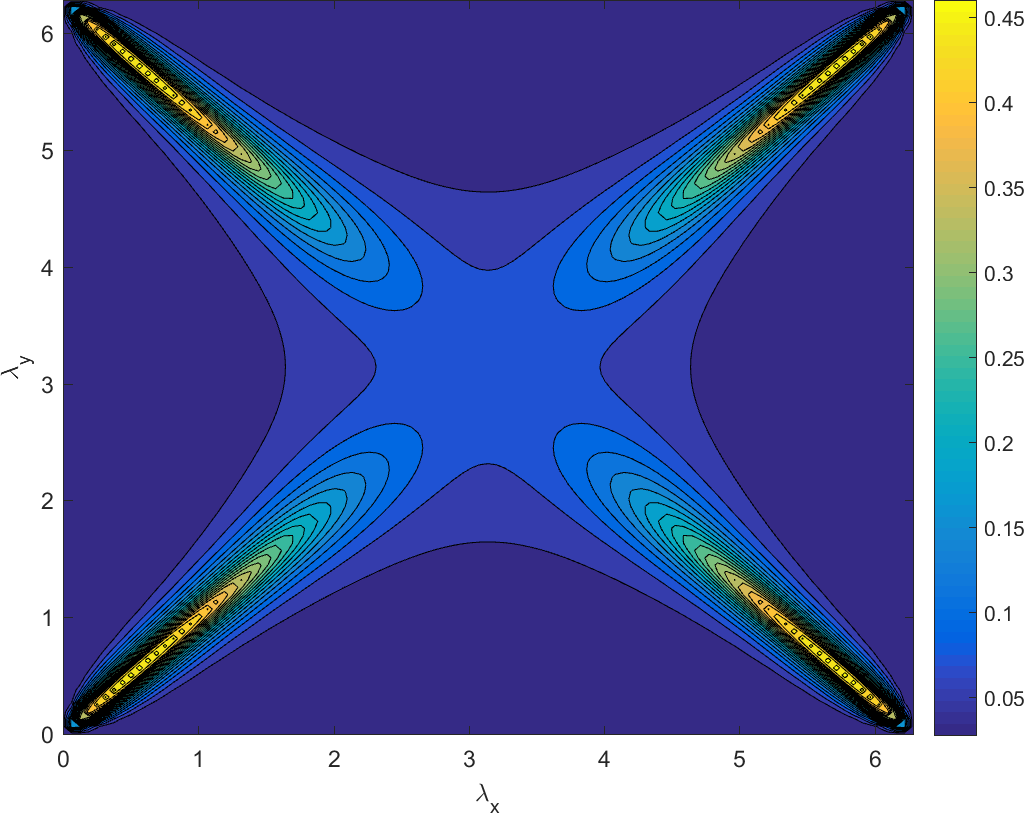
\includegraphics[width=0.975\textwidth]{figures/sec_DSA/SI_MIP_C=4_UPWLD1_LS2_x=1e-1_dydx=1_contour.png}
		\caption{$10^{-1}$ mfp}
	\end{subfigure}
	}
	\vspace{0.5cm}
	{
	\begin{subfigure}[b]{0.485\textwidth}
		\centering
		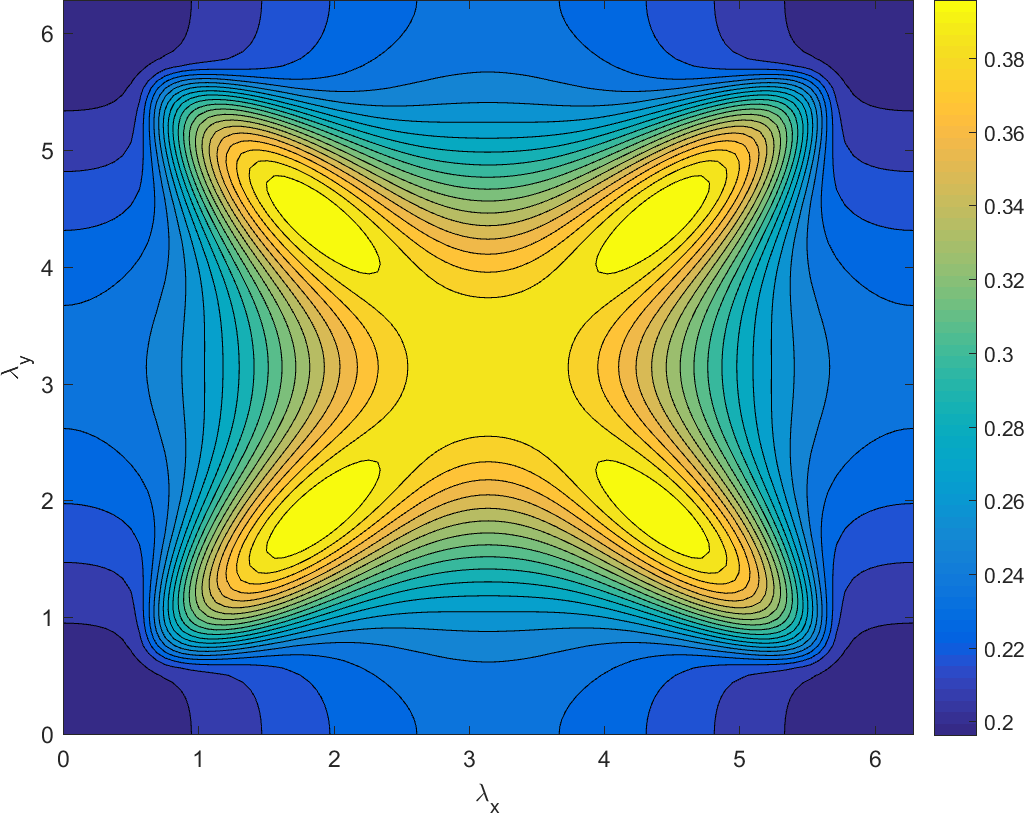
\includegraphics[width=0.975\textwidth]{figures/sec_DSA/SI_MIP_C=4_UPWLD1_LS2_x=1_dydx=1_contour.png}
		\caption{$10^{0}$ mfp}
	\end{subfigure}
	\hfill
	\begin{subfigure}[b]{0.485\textwidth}
		\centering
		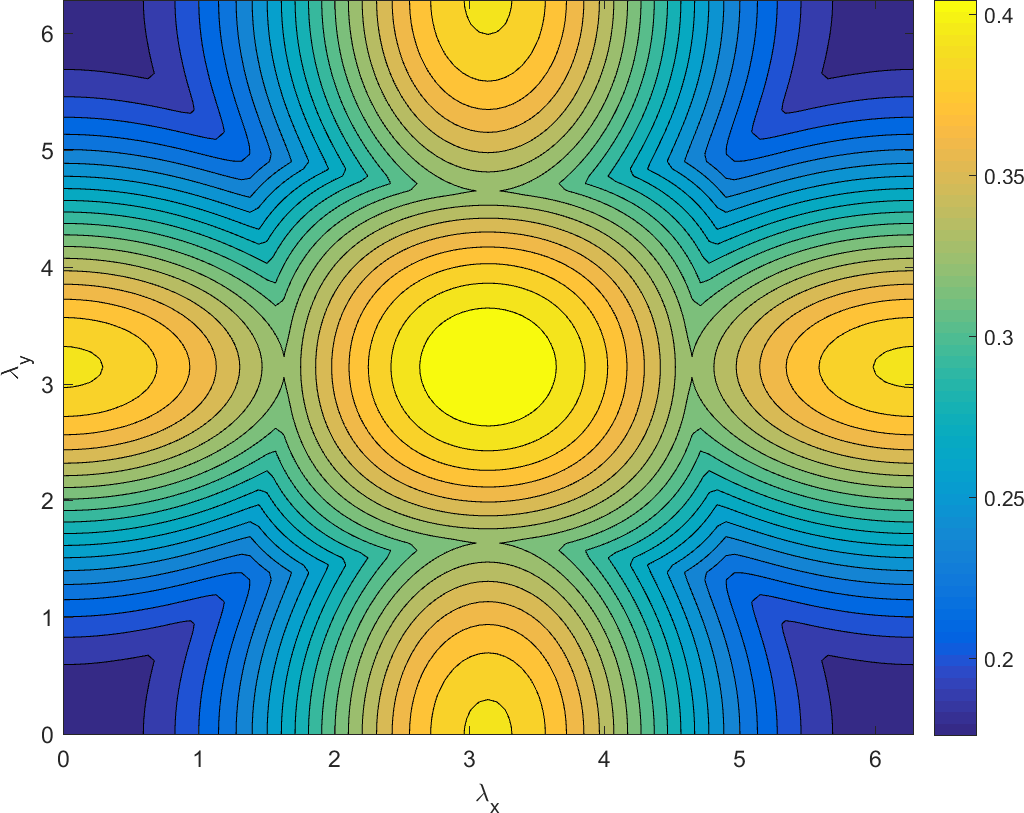
\includegraphics[width=0.975\textwidth]{figures/sec_DSA/SI_MIP_C=4_UPWLD1_LS2_x=10_dydx=1_contour.png}
		\caption{$10^{1}$ mfp}
	\end{subfigure}
	}
	\vspace{0.5cm}
	{
	\begin{subfigure}[b]{0.485\textwidth}
		\centering
		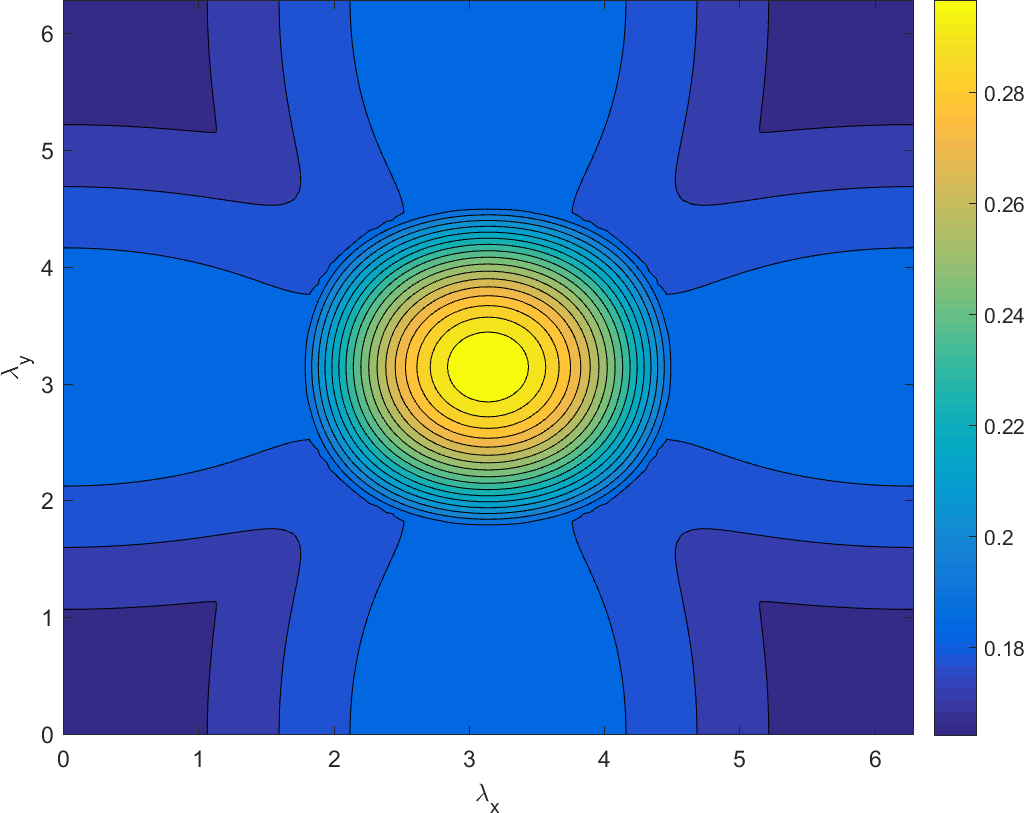
\includegraphics[width=0.975\textwidth]{figures/sec_DSA/SI_MIP_C=4_UPWLD1_LS2_x=100_dydx=1_contour.png}
		\caption{$10^{2}$ mfp}
	\end{subfigure}
	\hfill
	\begin{subfigure}[b]{0.485\textwidth}
		\centering
		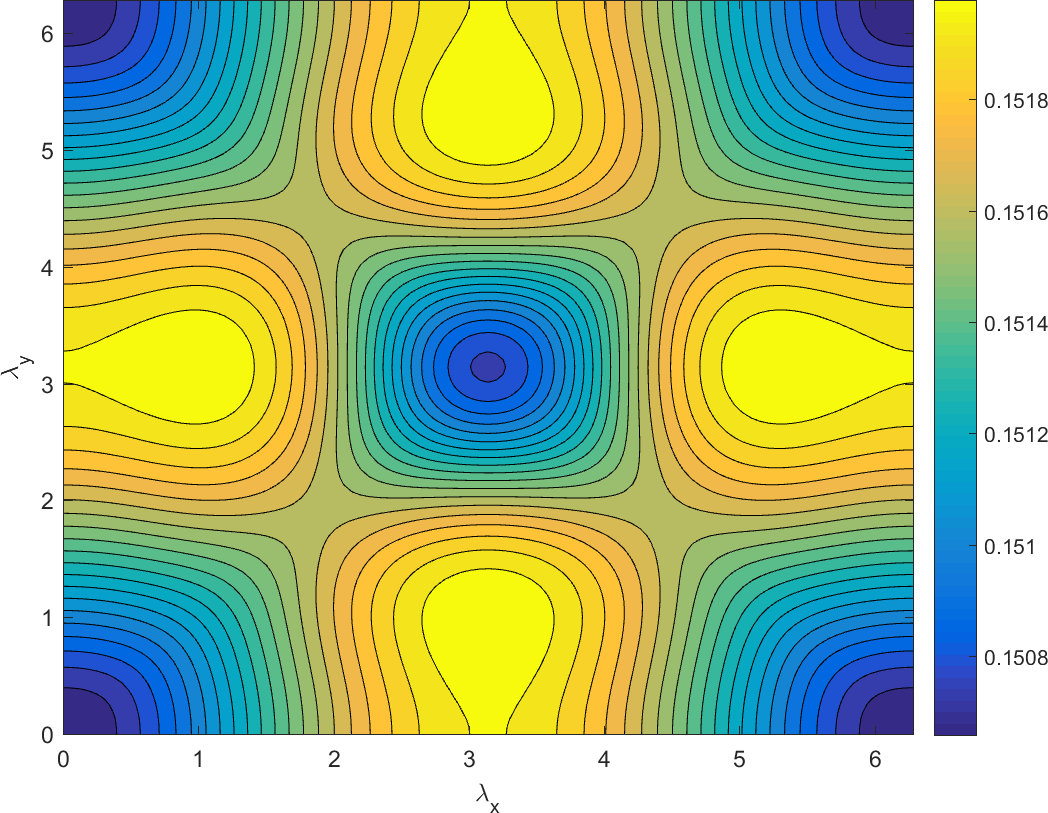
\includegraphics[width=0.975\textwidth]{figures/sec_DSA/SI_MIP_C=4_UPWLD1_LS2_x=1000_dydx=1_contour.png}
		\caption{$10^{3}$ mfp}
	\end{subfigure}
	}
\caption{Fourier wave number distribution for different mesh optical thicknesses of a single 2D square cell with PWL coordinates and LS2 quadrature.}
\label{fig::2D_homo_dsa_wave_LS2}
\end{figure}

\begin{figure}
\centering
	{
	\begin{subfigure}[b]{0.485\textwidth}
		\centering
		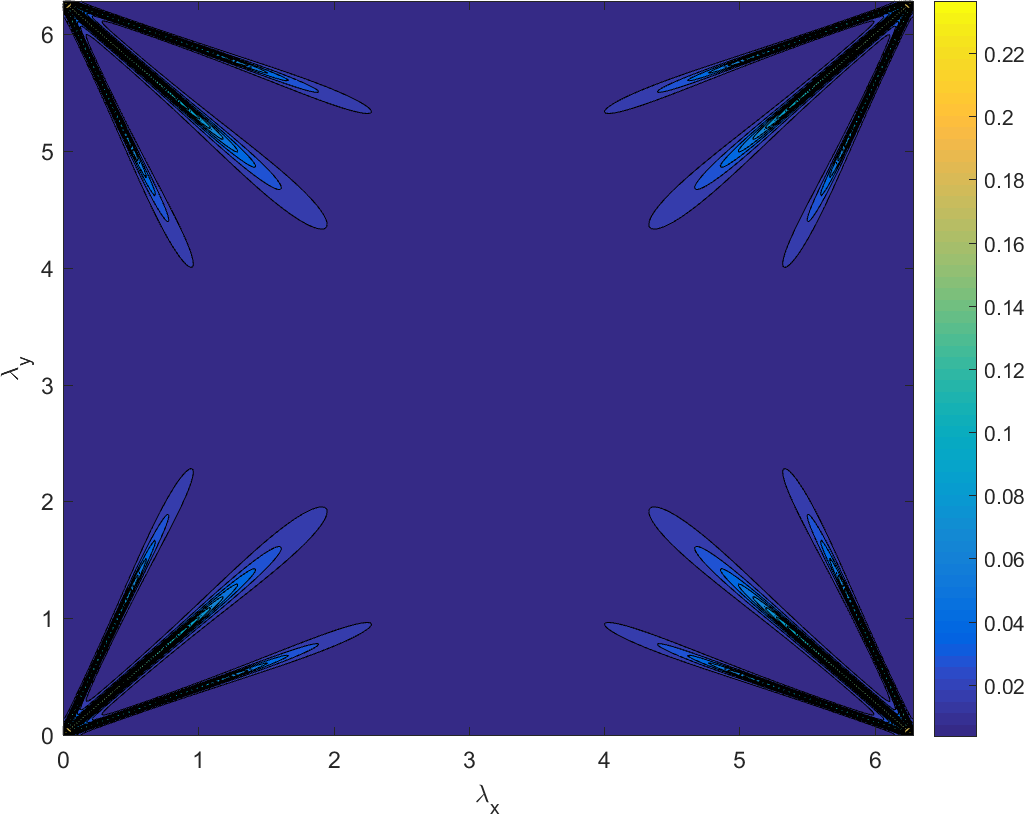
\includegraphics[width=0.975\textwidth]{figures/sec_DSA/SI_MIP_C=4_UPWLD1_LS4_x=1e-2_dydx=1_contour.png}
		\caption{$10^{-2}$ mfp}
	\end{subfigure}
	\hfill
	\begin{subfigure}[b]{0.485\textwidth}
		\centering
		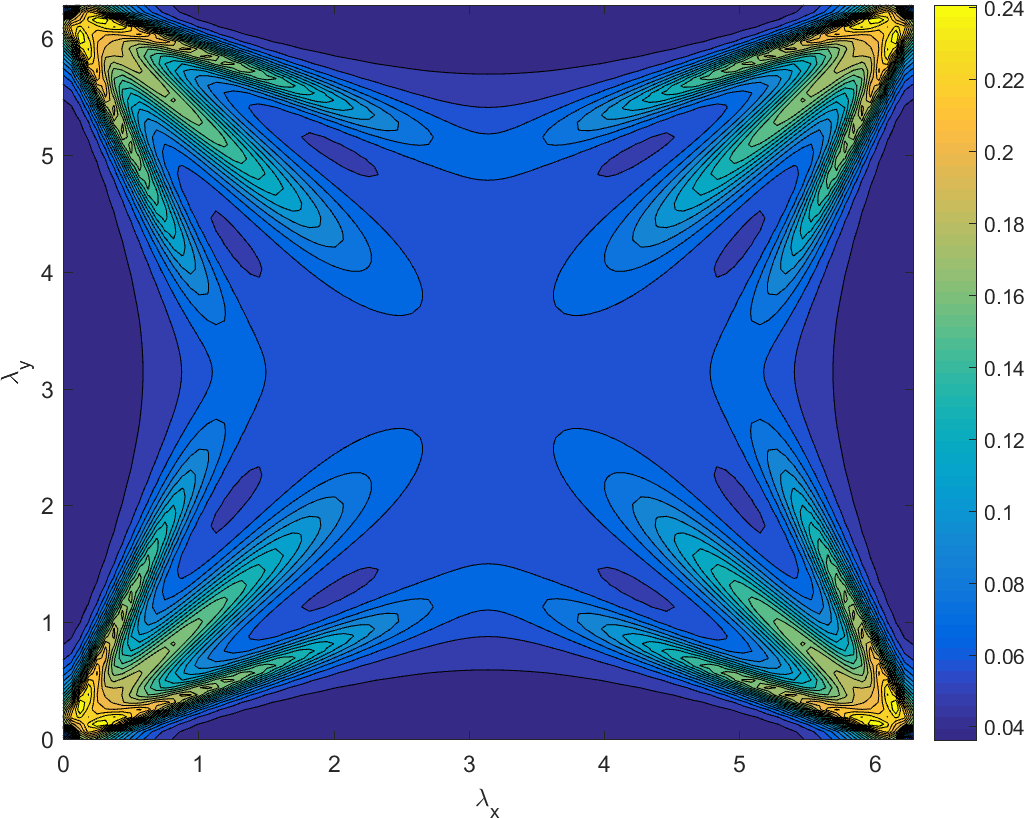
\includegraphics[width=0.975\textwidth]{figures/sec_DSA/SI_MIP_C=4_UPWLD1_LS4_x=1e-1_dydx=1_contour.png}
		\caption{$10^{-1}$ mfp}
	\end{subfigure}
	}
	\vspace{0.5cm}
	{
	\begin{subfigure}[b]{0.485\textwidth}
		\centering
		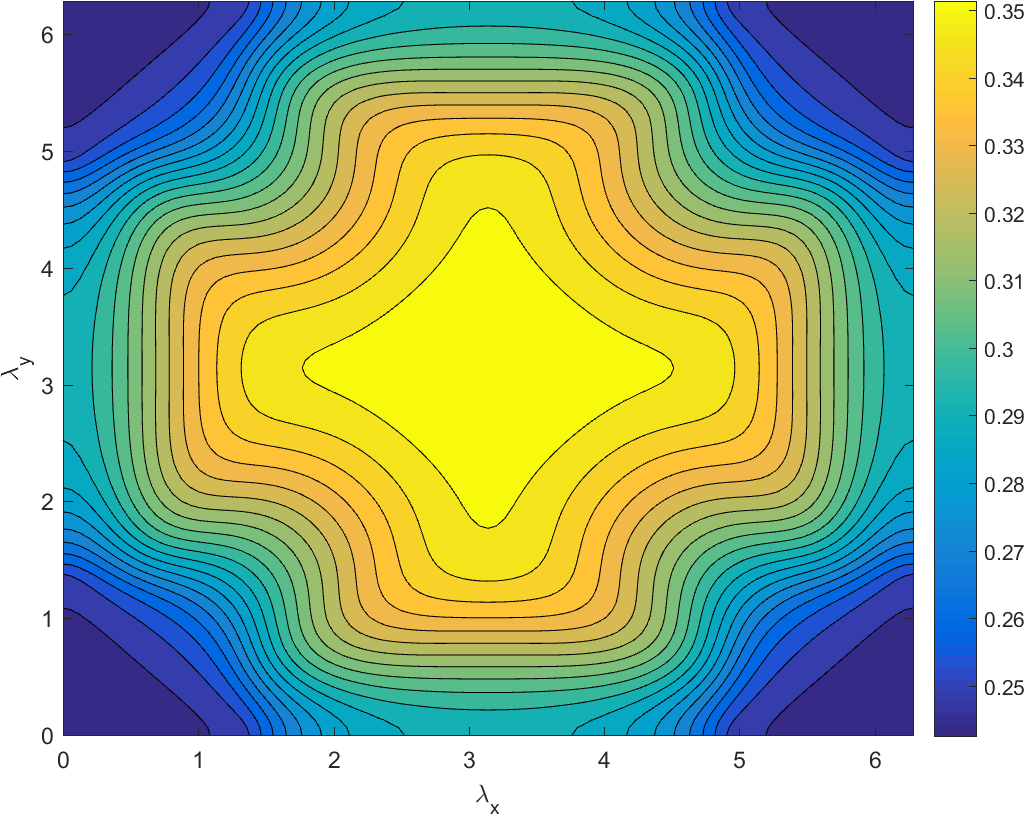
\includegraphics[width=0.975\textwidth]{figures/sec_DSA/SI_MIP_C=4_UPWLD1_LS4_x=1_dydx=1_contour.png}
		\caption{$10^{0}$ mfp}
	\end{subfigure}
	\hfill
	\begin{subfigure}[b]{0.485\textwidth}
		\centering
		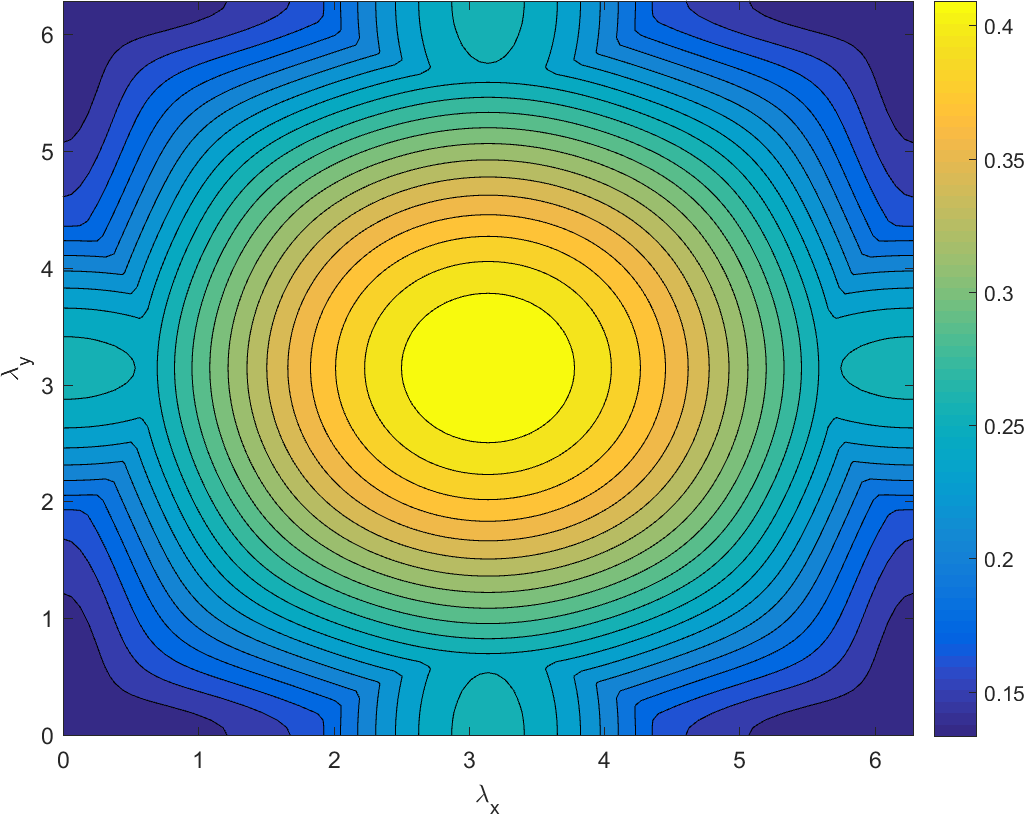
\includegraphics[width=0.975\textwidth]{figures/sec_DSA/SI_MIP_C=4_UPWLD1_LS4_x=10_dydx=1_contour.png}
		\caption{$10^{1}$ mfp}
	\end{subfigure}
	}
	\vspace{0.5cm}
	{
	\begin{subfigure}[b]{0.485\textwidth}
		\centering
		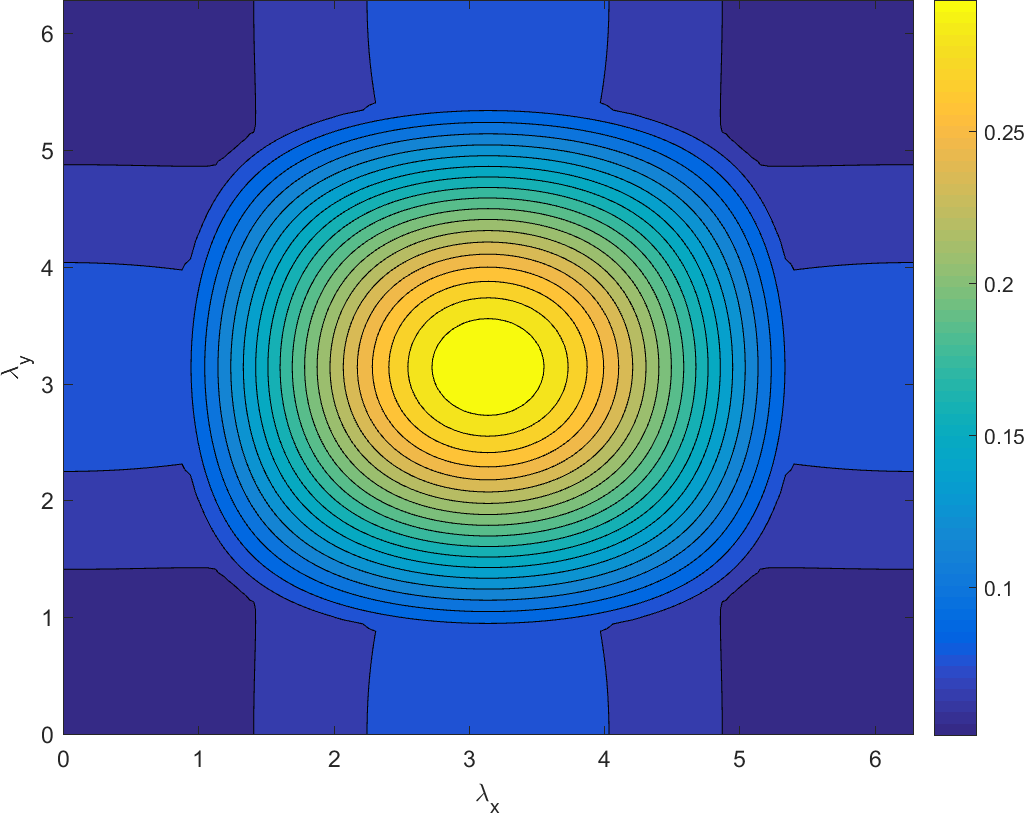
\includegraphics[width=0.975\textwidth]{figures/sec_DSA/SI_MIP_C=4_UPWLD1_LS4_x=100_dydx=1_contour.png}
		\caption{$10^{2}$ mfp}
	\end{subfigure}
	\hfill
	\begin{subfigure}[b]{0.485\textwidth}
		\centering
		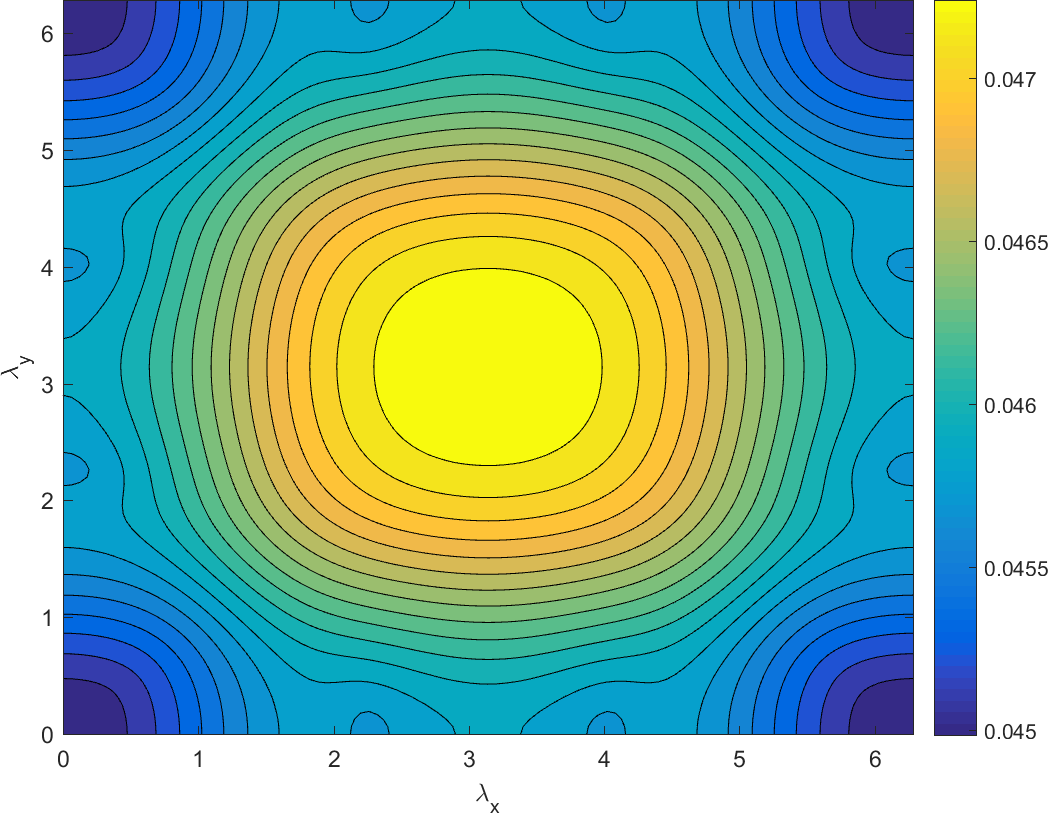
\includegraphics[width=0.975\textwidth]{figures/sec_DSA/SI_MIP_C=4_UPWLD1_LS4_x=1000_dydx=1_contour.png}
		\caption{$10^{3}$ mfp}
	\end{subfigure}
	}
\caption{Fourier wave number distribution for different mesh optical thicknesses of a single 2D square cell with PWL coordinates and LS4 quadrature.}
\label{fig::2D_homo_dsa_wave_LS4}
\end{figure}

\begin{figure}
\centering
	{
	\begin{subfigure}[b]{0.485\textwidth}
		\centering
		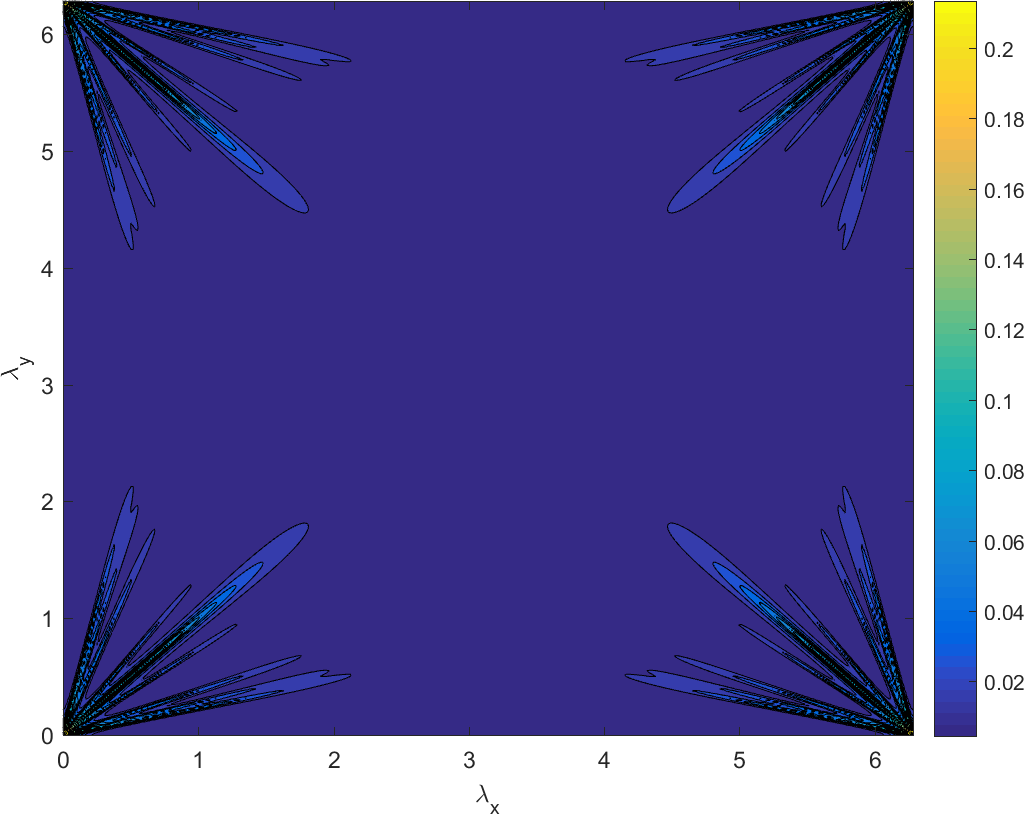
\includegraphics[width=0.975\textwidth]{figures/sec_DSA/SI_MIP_C=4_UPWLD1_LS8_x=1e-2_dydx=1_contour.png}
		\caption{$10^{-2}$ mfp}
	\end{subfigure}
	\hfill
	\begin{subfigure}[b]{0.485\textwidth}
		\centering
		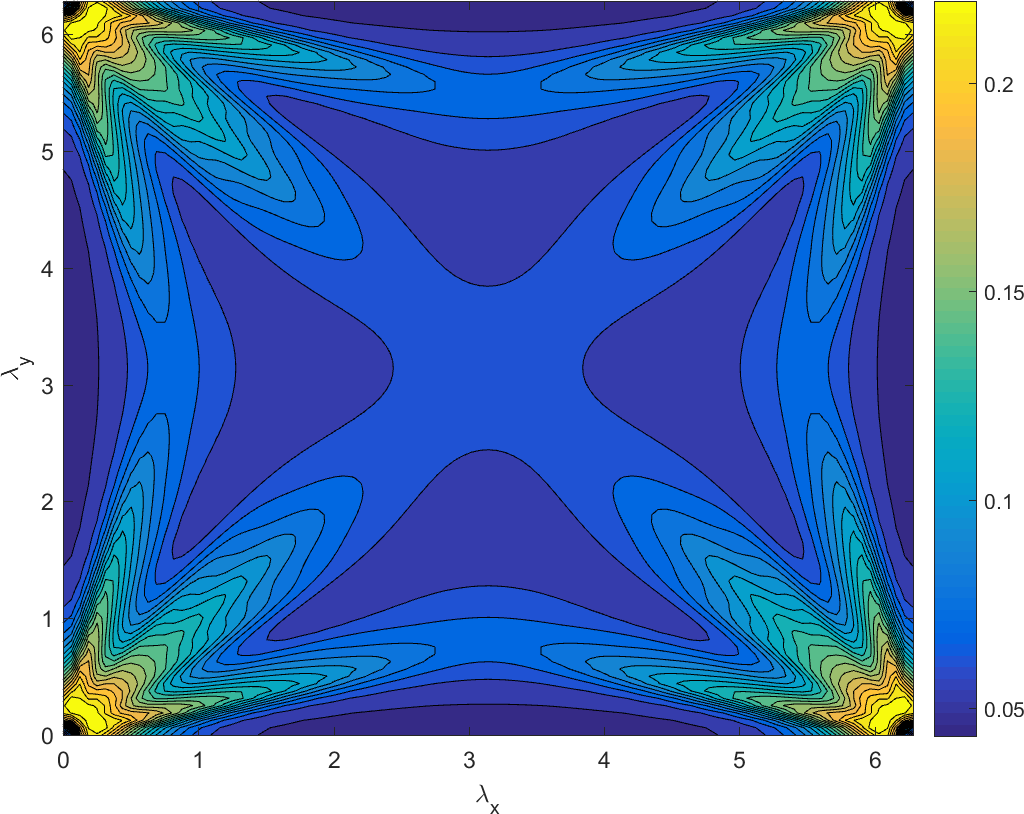
\includegraphics[width=0.975\textwidth]{figures/sec_DSA/SI_MIP_C=4_UPWLD1_LS8_x=1e-1_dydx=1_contour.png}
		\caption{$10^{-1}$ mfp}
	\end{subfigure}
	}
	\vspace{0.5cm}
	{
	\begin{subfigure}[b]{0.485\textwidth}
		\centering
		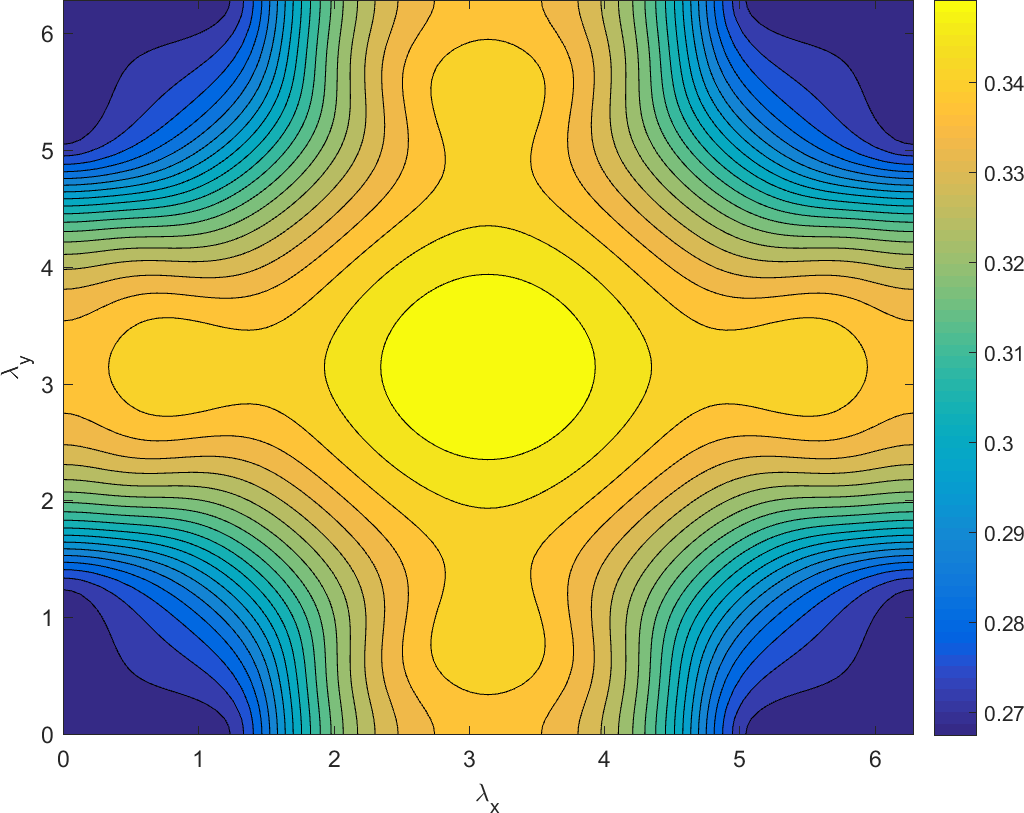
\includegraphics[width=0.975\textwidth]{figures/sec_DSA/SI_MIP_C=4_UPWLD1_LS8_x=1_dydx=1_contour.png}
		\caption{$10^{0}$ mfp}
	\end{subfigure}
	\hfill
	\begin{subfigure}[b]{0.485\textwidth}
		\centering
		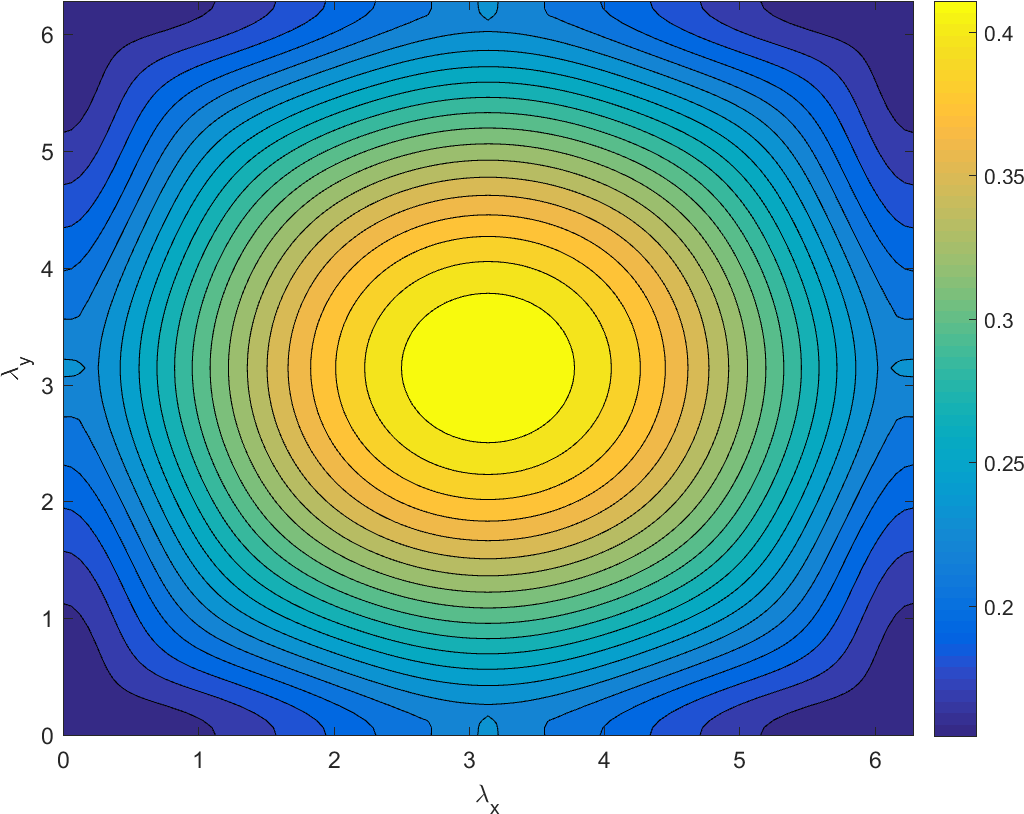
\includegraphics[width=0.975\textwidth]{figures/sec_DSA/SI_MIP_C=4_UPWLD1_LS8_x=10_dydx=1_contour.png}
		\caption{$10^{1}$ mfp}
	\end{subfigure}
	}
	\vspace{0.5cm}
	{
	\begin{subfigure}[b]{0.485\textwidth}
		\centering
		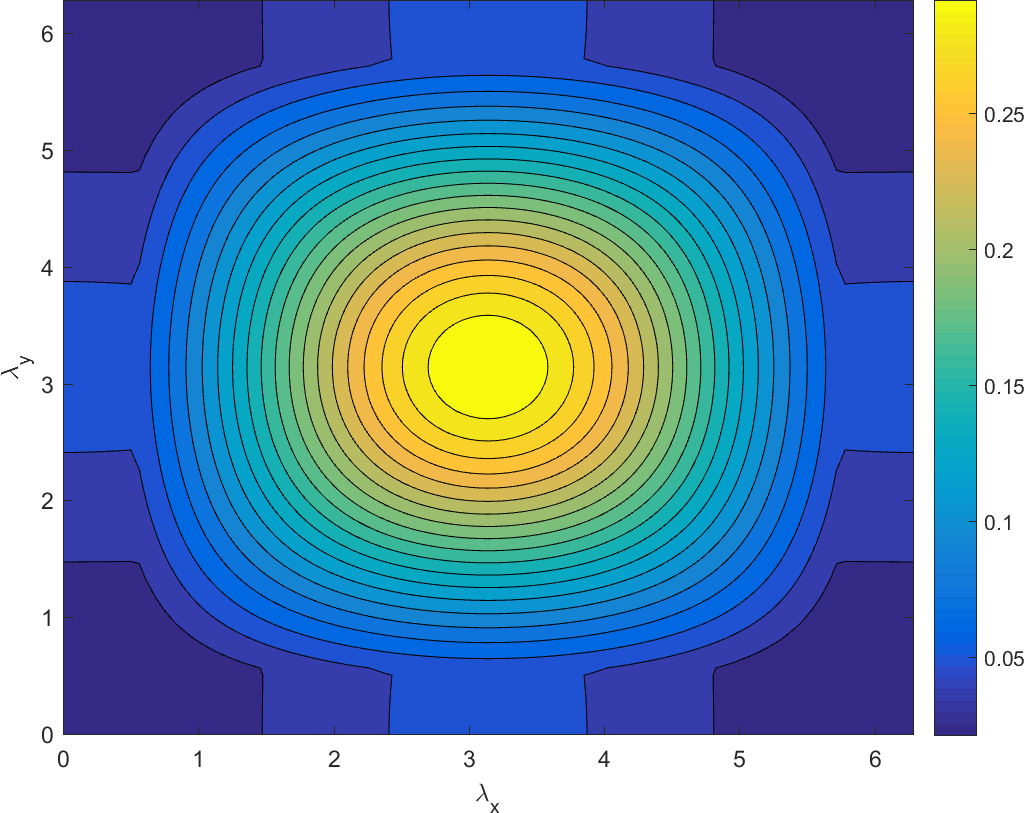
\includegraphics[width=0.975\textwidth]{figures/sec_DSA/SI_MIP_C=4_UPWLD1_LS8_x=100_dydx=1_contour.png}
		\caption{$10^{2}$ mfp}
	\end{subfigure}
	\hfill
	\begin{subfigure}[b]{0.485\textwidth}
		\centering
		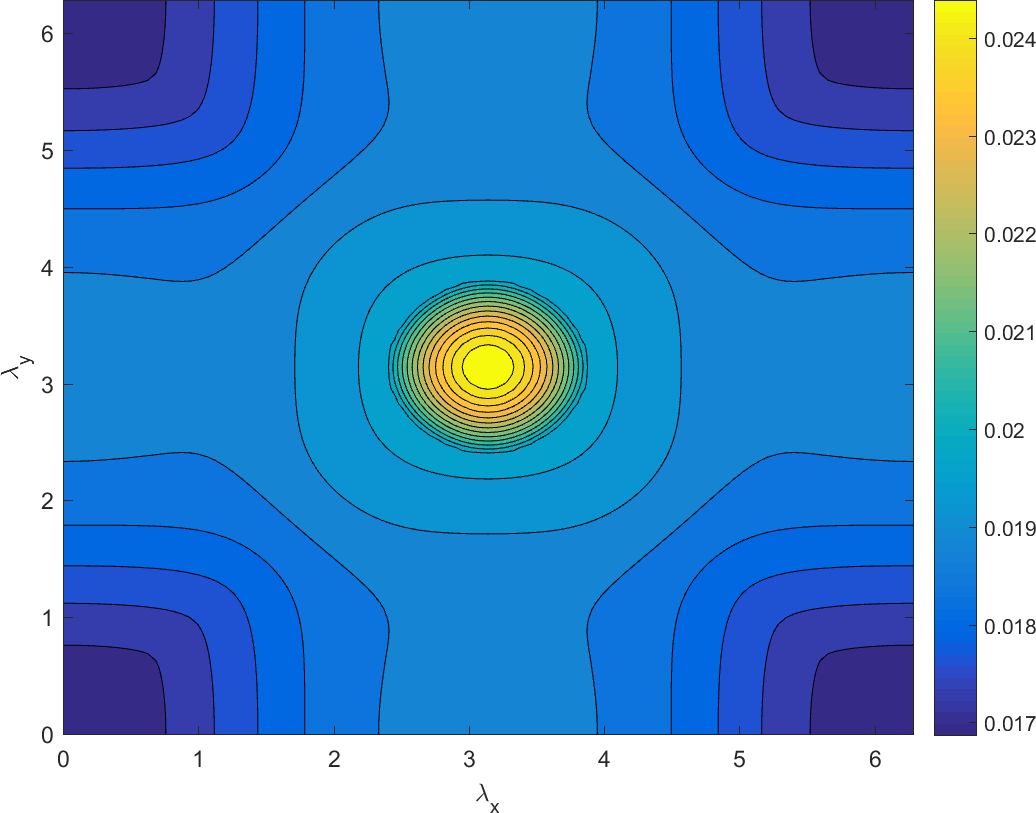
\includegraphics[width=0.975\textwidth]{figures/sec_DSA/SI_MIP_C=4_UPWLD1_LS8_x=1000_dydx=1_contour.png}
		\caption{$10^{3}$ mfp}
	\end{subfigure}
	}
\caption{Fourier wave number distribution for different mesh optical thicknesses of a single 2D square cell with PWL coordinates and LS8 quadrature.}
\label{fig::2D_homo_dsa_wave_LS8}
\end{figure}

%%%%%%%%%%%%%%%%%%%%%%%%%%%%%%%%%%%%%%%%%%%%%%%%%%%
%%%   SubSubSection -  3D Homogeneous Medium
\subsubsection{3D Homogeneous Medium Case}
\label{sec::DSA_Results_1G_3DHomo}

\begin{figure}
\centering
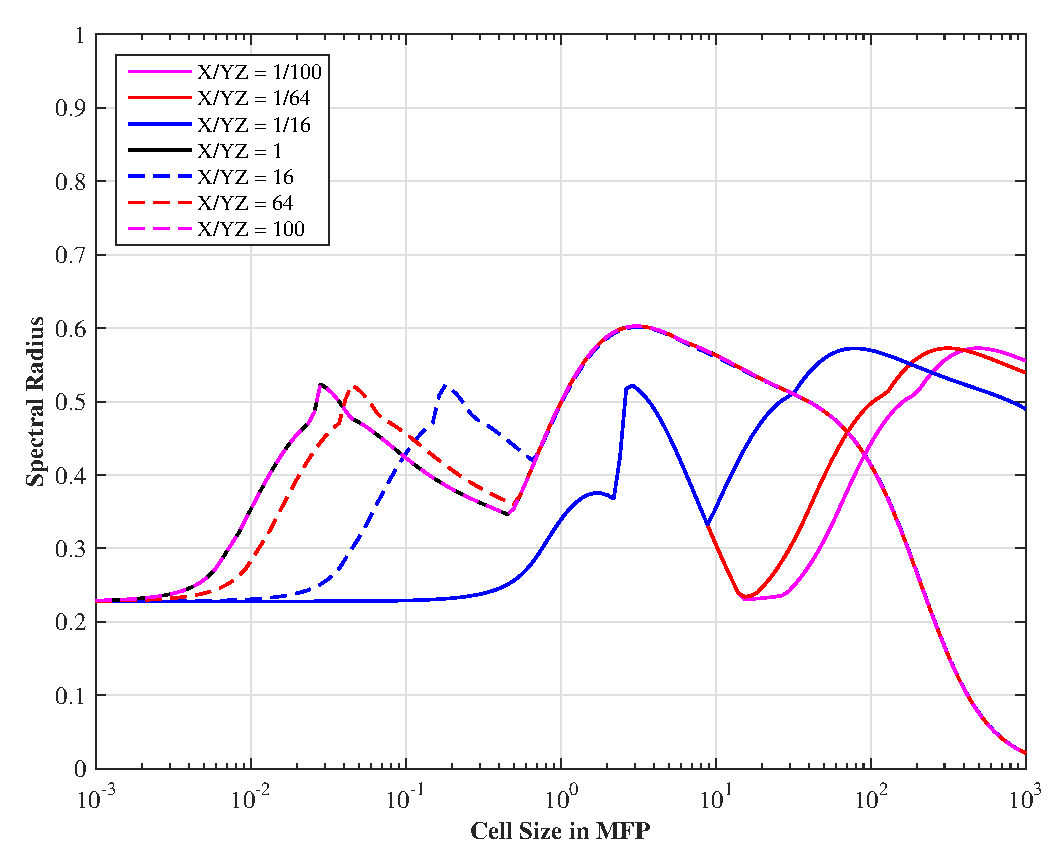
\includegraphics[width=0.75\textwidth]{figures/sec_DSA/SI_MIP_hex_PWLD1_AR1.eps}
\caption{Fourier spectral radii for MIP with 3D PWL coordinates with different aspect ratios and $c=1$.}
\label{fig::DSA_1G_Fourier_PWL_AR1}
\end{figure}

\begin{figure}
\centering
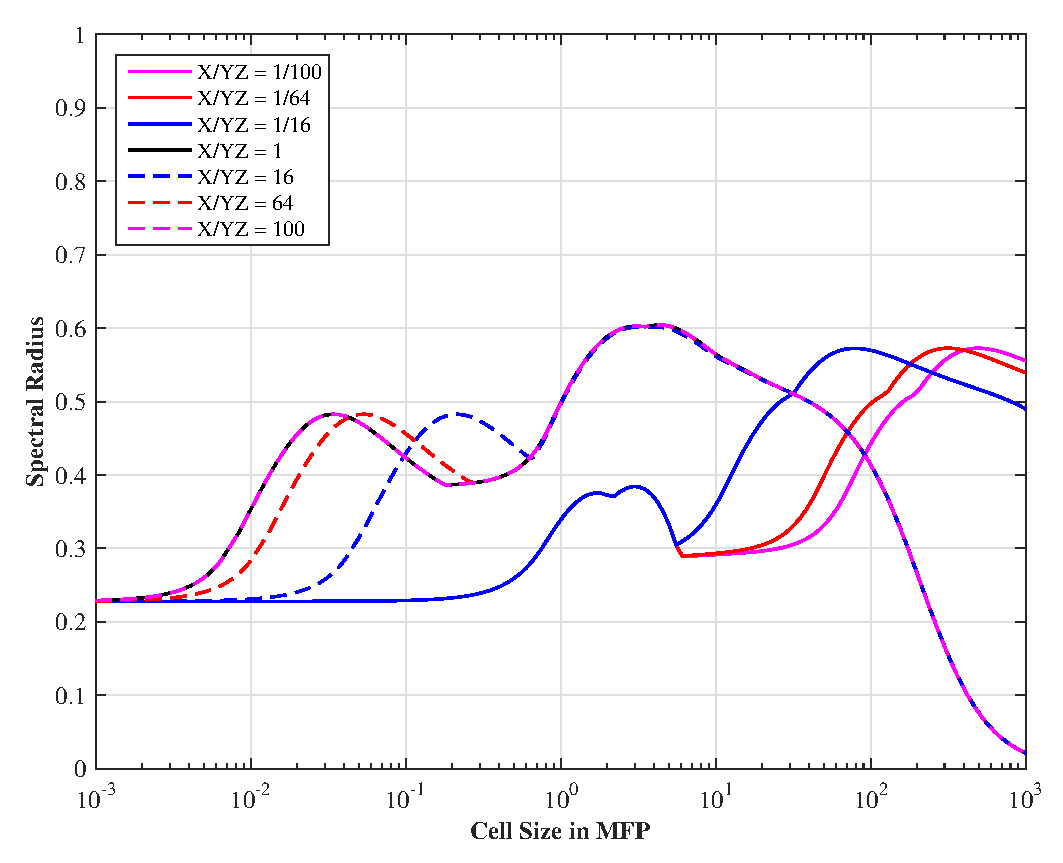
\includegraphics[width=0.75\textwidth]{figures/sec_DSA/SI_MIP_hex_PWLD1_AR4.eps}
\caption{Fourier spectral radii for MIP with 3D PWL coordinates with different aspect ratios and $c=4$.}
\label{fig::DSA_1G_Fourier_PWL_AR4}
\end{figure}

%%%%%%%%%%%%%%%%%%%%%%%%%%%%%%%%%%%%%%%%%%%%%%%%%%%
%%%   SubSubSection -  PHI
\subsubsection{Periodic Horizontal Interface Problem}
\label{sec::DSA_Results_1G_PHI}

When DSA is applied to multidimensional problems (2D and 3D), the preconditioning of the transport operators can degrade in the presence of heterogeneous configurations with large material discontinuities \cite{azmy2002unconditionally}. The Periodic Horizontal Interface (PHI) problem is considered a litmus test for heterogeneous DSA techniques. This problem consists of horizontal strips of alternating optically thick and optically thin materials that are 1 cell in depth. We define $\sigma_1$ as the optically thick total cross section and $\sigma_2$ as the optically thin total cross section. We then define a tuning parameter, $\sigma$, and allow the region cross sections to have the following form:

\begin{equation}
\begin{aligned}
\sigma_1 &= \sigma \\
\sigma_2 &= \frac{1}{\sigma}
\end{aligned}.
\end{equation}

\noindent We can see that increasing the value of $\sigma$ will increase the magnitude of difference between the two region cross sections. Therefore, as $\sigma$ grows large, the material discontinuities will grow which could potentially reduce the performance of our DSA scheme.

From the analysis presented in Section \ref{sec::DSA_Results_1G_2DHomo}, we showed that our different 2D linear and quadratic basis functions were robust and stable, even for mesh cells with large aspect ratios. For this PHI analysis, we concentrate on analyzing just the linear PWL coordinates as our basis functions. Just like before, we will also examine different level-symmetric quadrature sets and their effects problems with varying optical thickness. The optical thickness and diffusivity of the problem is increased by varying both $\sigma$ and the scattering ratio, $c$. This study was conducted with the sequence, $\sigma = \left[ 10, 20, 40, 80, 160, 320, 640  \right]$, and with following scattering ratios: $c = \left[ 0.9,0.99,0.999,0.9999,0.99999,0.999999  \right]$.

The full results of this PHI analysis are presented in Tables \ref{tab::DSA_2DPHI_LS2} - \ref{tab::DSA_2DPHI_LS16} for the LS2, LS4, LS8, and LS16 quadratures, respectively. From these tables, we can see that MIP DSA loses its effectiveness as the heterogeneity and overall diffusivity of the problem increases. The theoretical spectral radii are greater than any of the values presented for the homogeneous case from Figure \ref{fig::DSA_1G_Fourier_PWL1}. This result is true even for the example with the smallest heterogeneity and smallest diffusivity ($\sigma=10$ and $c=0.9$). We can gain some more knowledge of the DSA degradation by observing the eigenvalue dependency on the fourier wave numbers for our problems. Figure \ref{fig::PHI_sig=10_c=0.9} provides the eigenvalue distribution based off the fourier wave numbers for the different quadrature sets for $\sigma=10$ and $c=0.9$. Figure \ref{fig::PHI_sig=640_c=0.9999} then provides the same information for $\sigma=640$ and $c=0.9999$.

\begin{table}
\caption{Spectral radius for the 2D PHI problem with the PWL basis functions and LS2 quadrature.}
\begin{center}
\def\arraystretch{1.6}
\begin{tabular}{|c|c|c|c|c|c|c|}
\hline
& \multicolumn{6}{c}{Scattering ratios}\vline\\
\hline
$\sigma$ & 0.9 & 0.99& 0.999& 0.9999& 0.99999& 0.99999 \\
\hline
10  &0.77091&0.89908&0.91279&0.91417&0.91431&0.91432 \\
20  &0.82038&0.94425&0.95859&0.96003&0.96018&0.96019  \\
40  &0.84803&0.96525&0.97982&0.98129&0.98144&0.98145  \\
80  &0.86188&0.97491&0.98955&0.99102&0.99117&0.99119  \\
160&0.87134&0.98003&0.99409&0.99557&0.99571&0.99573  \\
320&0.87833&0.98353&0.99626&0.99774&0.99789&0.99790  \\
640&0.88187&0.98533&0.99732&0.99880&0.99894&0.99896  \\
\hline
\end{tabular}
\end{center}
\label{tab::DSA_2DPHI_LS2}
\end{table}

\begin{table}
\caption{Spectral radius for the 2D PHI problem with the PWL basis functions and LS4 quadrature.}
\begin{center}
\def\arraystretch{1.6}
\begin{tabular}{|c|c|c|c|c|c|c|}
\hline
& \multicolumn{6}{c}{Scattering ratios}\vline\\
\hline
$\sigma$ & 0.9 & 0.99& 0.999& 0.9999& 0.99999& 0.99999 \\
\hline
10  &0.74609&0.87284&0.88970&0.89148&0.89166&0.89167\\
20  &0.81135&0.93358&0.95001&0.95179&0.95197&0.95199\\
40  &0.84353&0.96104&0.97612&0.97781&0.97799&0.97800\\
80  &0.85865&0.97342&0.98785&0.98943&0.98960&0.98961\\
160&0.86998&0.97913&0.99335&0.99482&0.99497&0.99499\\
320&0.87767&0.98307&0.99593&0.99739&0.99753&0.99755\\
640&0.88166&0.98500&0.99717&0.99863&0.99878&0.99879\\
\hline
\end{tabular}
\end{center}
\label{tab::DSA_2DPHI_LS4}
\end{table}

\begin{table}
\caption{Spectral radius for the 2D PHI problem with the PWL basis functions and LS8 quadrature.}
\begin{center}
\def\arraystretch{1.6}
\begin{tabular}{|c|c|c|c|c|c|c|}
\hline
& \multicolumn{6}{c}{Scattering ratios}\vline\\
\hline
$\sigma$ & 0.9 & 0.99& 0.999& 0.9999& 0.99999& 0.99999 \\
\hline
10  &0.75532&0.87917&0.89780&0.89989&0.90010&0.90012\\
20  &0.81754&0.93694&0.95380&0.95581&0.95602&0.95604\\
40  &0.84681&0.96337&0.97793&0.97969&0.97988&0.97990\\
80  &0.86032&0.97459&0.98898&0.99042&0.99057&0.99058\\
160&0.86980&0.98007&0.99394&0.99540&0.99554&0.99556\\
320&0.87795&0.98354&0.99623&0.99768&0.99783&0.99784\\
640&0.88204&0.98524&0.99732&0.99878&0.99892&0.99894\\
\hline
\end{tabular}
\end{center}
\label{tab::DSA_2DPHI_LS8}
\end{table}

\begin{table}
\caption{Spectral radius for the 2D PHI problem with the PWL basis functions and LS16 quadrature.}
\begin{center}
\def\arraystretch{1.6}
\begin{tabular}{|c|c|c|c|c|c|c|}
\hline
& \multicolumn{6}{c}{Scattering ratios}\vline\\
\hline
$\sigma$ & 0.9 & 0.99& 0.999& 0.9999& 0.99999& 0.99999 \\
\hline
10  &0.75796&0.88052&0.89888&0.90097&0.90119&0.90121\\
20  &0.81903&0.93790&0.95455&0.95651&0.95671&0.95673\\
40  &0.84758&0.96387&0.97842&0.98015&0.98033&0.98035\\
80  &0.86070&0.97485&0.98924&0.99069&0.99083&0.99085\\
160&0.87025&0.98029&0.99407&0.99553&0.99567&0.99569\\
320&0.87817&0.98365&0.99629&0.99775&0.99790&0.99791\\
640&0.88216&0.98530&0.99735&0.99881&0.99896&0.99897\\
\hline
\end{tabular}
\end{center}
\label{tab::DSA_2DPHI_LS16}
\end{table}

\begin{figure}
\centering
	{
	\begin{subfigure}[b]{0.485\textwidth}
		\centering
		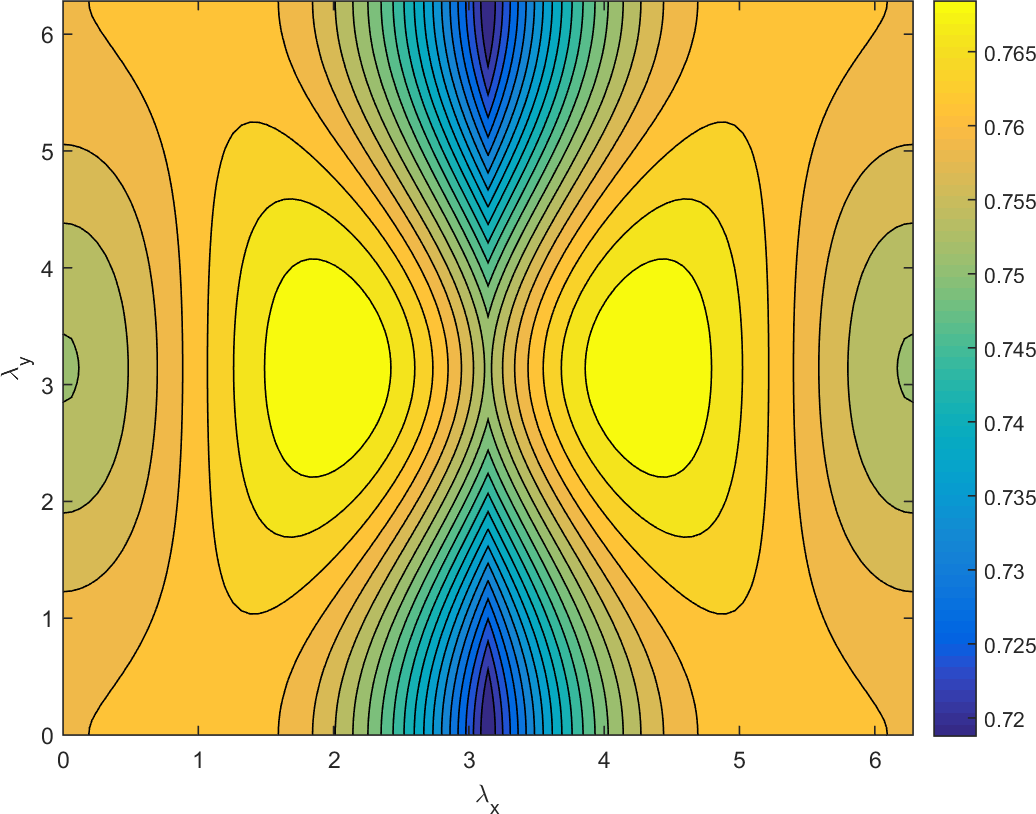
\includegraphics[width=0.975\textwidth]{figures/sec_DSA/PHI_SI_MIP_C=4_UPWLD1_LS2_sigt=10_c=9_contour.png}
		\caption{LS2}
	\end{subfigure}
	\hfill
	\begin{subfigure}[b]{0.485\textwidth}
		\centering
		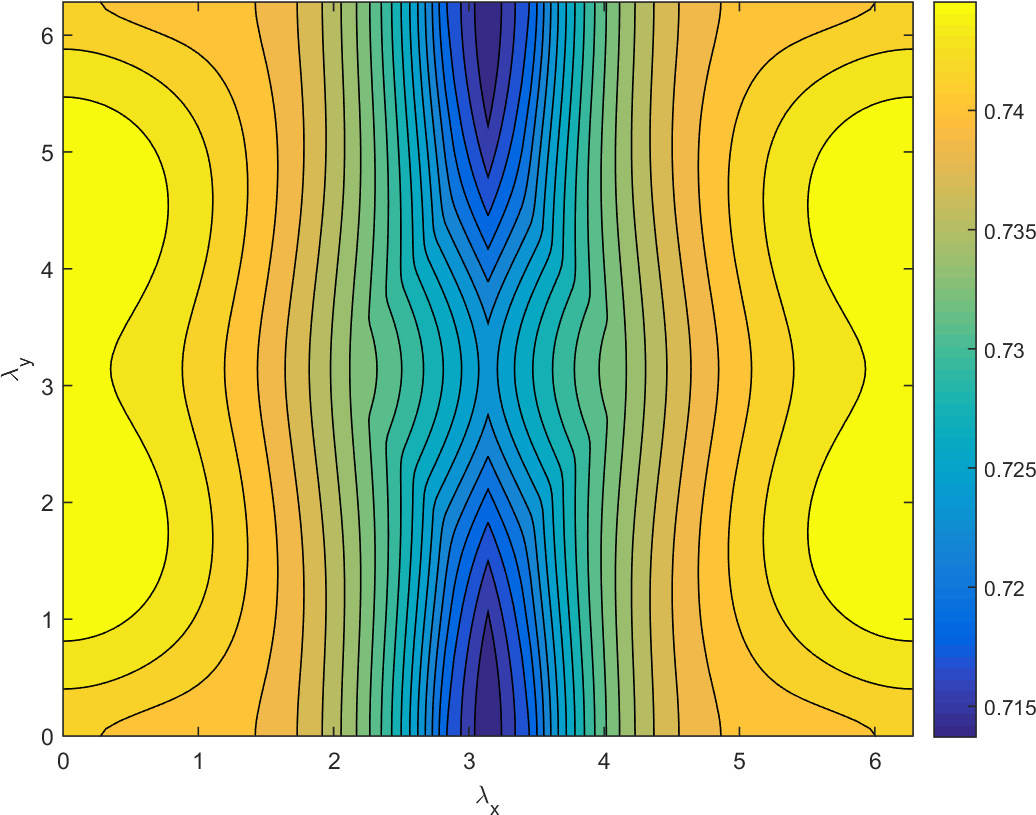
\includegraphics[width=0.975\textwidth]{figures/sec_DSA/PHI_SI_MIP_C=4_UPWLD1_LS4_sigt=10_c=9_contour.png}
		\caption{LS4}
	\end{subfigure}
	}
	\vspace{1.5cm}
	{
	\begin{subfigure}[b]{0.485\textwidth}
		\centering
		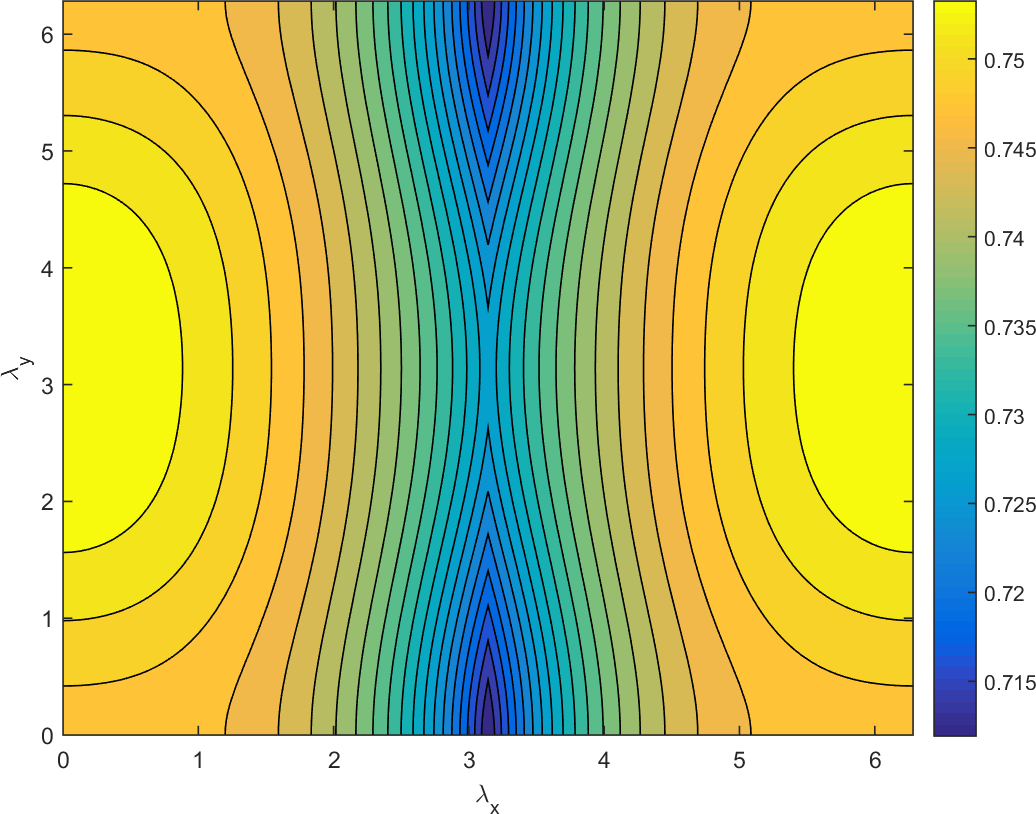
\includegraphics[width=0.975\textwidth]{figures/sec_DSA/PHI_SI_MIP_C=4_UPWLD1_LS8_sigt=10_c=9_contour.png}
		\caption{LS8}
	\end{subfigure}
	\hfill
	\begin{subfigure}[b]{0.485\textwidth}
		\centering
		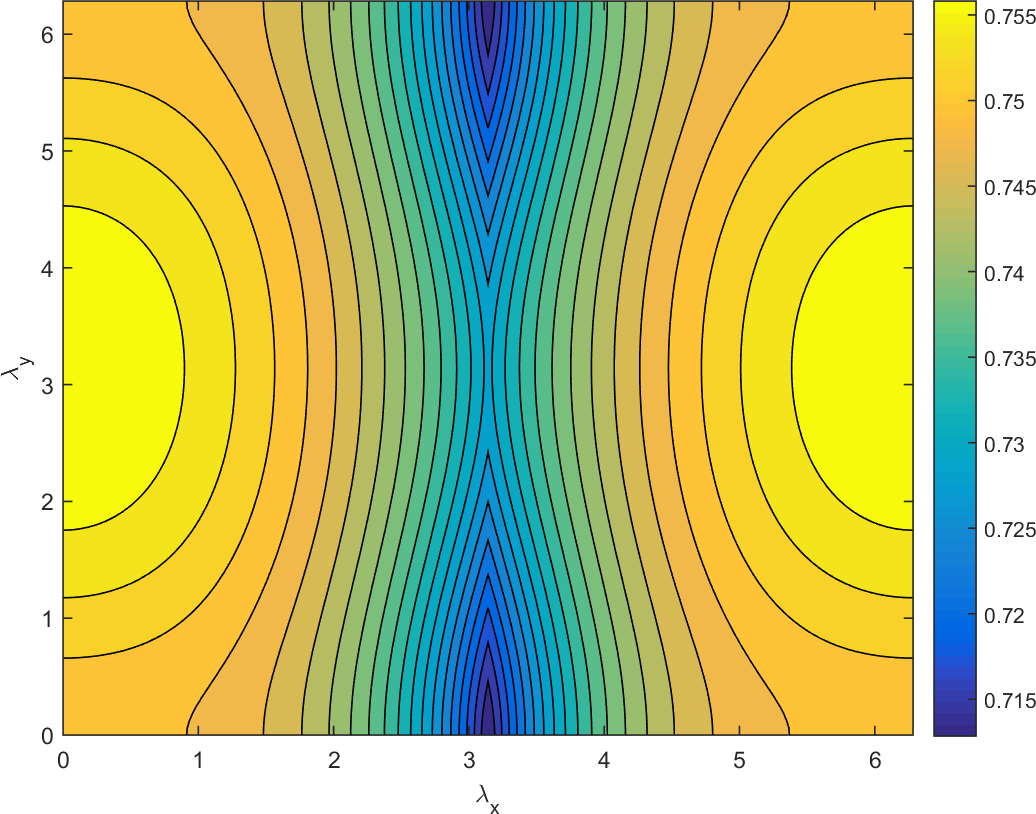
\includegraphics[width=0.975\textwidth]{figures/sec_DSA/PHI_SI_MIP_C=4_UPWLD1_LS16_sigt=10_c=9_contour.png}
		\caption{LS16}
	\end{subfigure}
	}
\caption{Fourier wave number distribution for the 2D PHI problem with $\sigma=10$ and $c=0.9$ and different level-symmetric quadratures.}
\label{fig::PHI_sig=10_c=0.9}
\end{figure}

\begin{figure}
\centering
	{
	\begin{subfigure}[b]{0.485\textwidth}
		\centering
		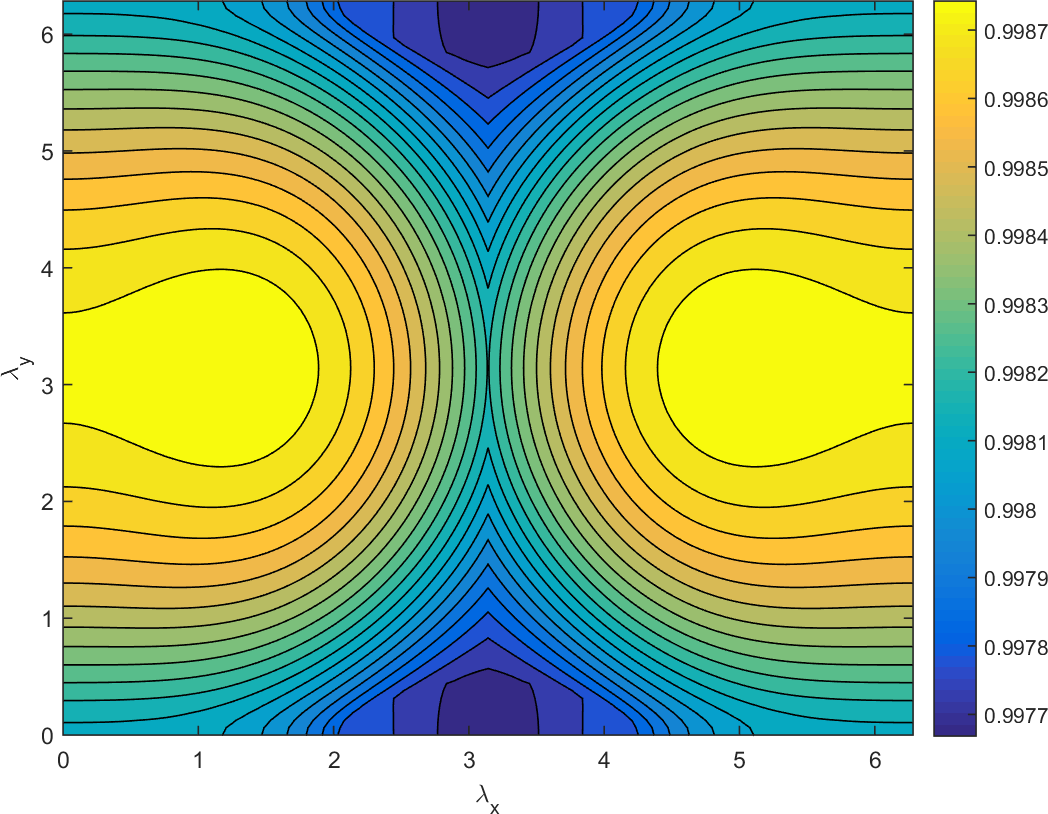
\includegraphics[width=0.975\textwidth]{figures/sec_DSA/PHI_SI_MIP_C=4_UPWLD1_LS2_sigt=640_c=9999_contour.png}
		\caption{LS2}
	\end{subfigure}
	\hfill
	\begin{subfigure}[b]{0.485\textwidth}
		\centering
		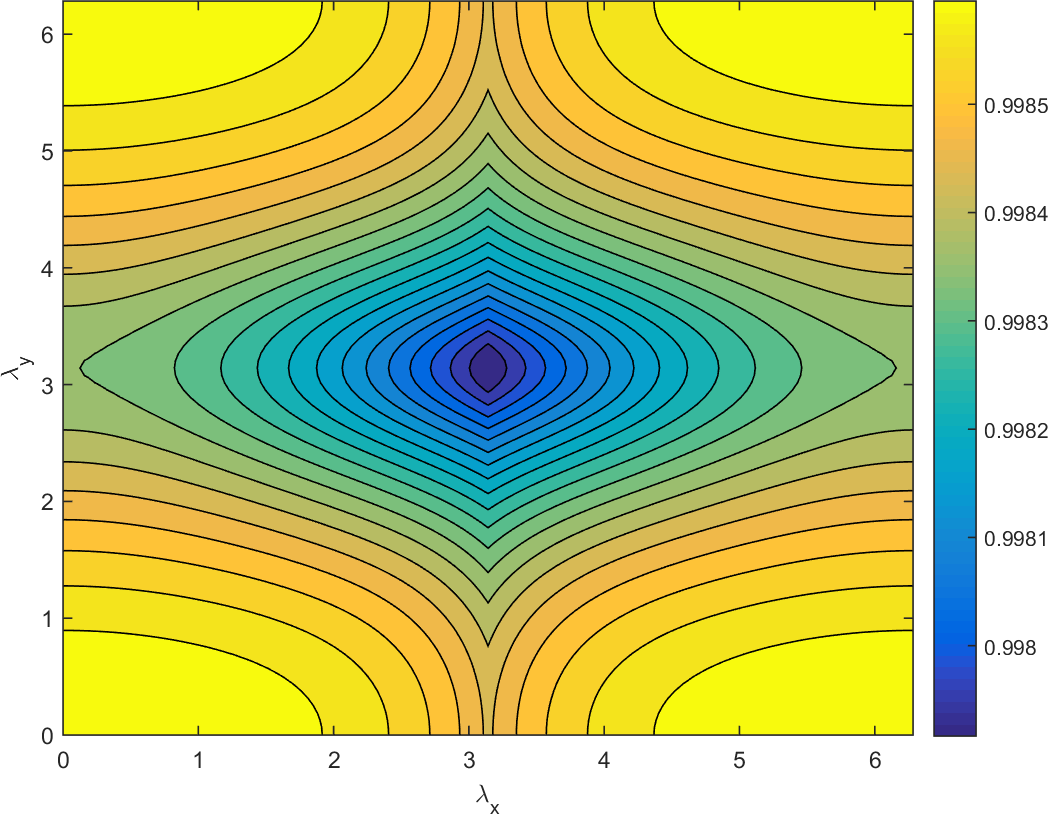
\includegraphics[width=0.975\textwidth]{figures/sec_DSA/PHI_SI_MIP_C=4_UPWLD1_LS4_sigt=640_c=9999_contour.png}
		\caption{LS4}
	\end{subfigure}
	}
	\vspace{1.5cm}
	{
	\begin{subfigure}[b]{0.485\textwidth}
		\centering
		\includegraphics[width=0.975\textwidth]{figures/sec_DSA/PHI_SI_MIP_C=4_UPWLD1_LS8_sigt=640_c=9999_contour.png}
		\caption{LS8}
	\end{subfigure}
	\hfill
	\begin{subfigure}[b]{0.485\textwidth}
		\centering
		\includegraphics[width=0.975\textwidth]{figures/sec_DSA/PHI_SI_MIP_C=4_UPWLD1_LS16_sigt=640_c=9999_contour.png}
		\caption{LS16}
	\end{subfigure}
	}
\caption{Fourier wave number distribution for the 2D PHI problem with $\sigma=640$ and $c=0.9999$ and different level-symmetric quadratures.}
\label{fig::PHI_sig=640_c=0.9999}
\end{figure}

%%%%%%%%%%%%%%%%%%%%%%%%%%%%%%%%%%%%%%%%%%%%%%%%%%%
%%%   SubSubSection -  AMR Iron Water
\subsubsection{Performance of MIP DSA with Adaptive Mesh Refinement}
\label{sec::DSA_Results_1G_AMR}

For the final theoretical analysis of DSA with the MIP form, we analyze the acceleration performance when AMR is utilized on a sufficiently optically thick transport with material discontinuities. The 2D transport problem that will be examined is similar to the Iron-Water problem \cite{khalil1985nodal}. It was modified by Wang and Ragusa for use with higher-order basis functions on triangular meshes with hanging nodes \cite{ref::DSA_wang_ragusa}. We will reexamine their work on degenarate polygonal grids and not use hanging nodes. The complete geometric desciption of our problem including boundary conditions and material distributions is given in Figure \ref{fig::DSA_IW_Description}. The material properties for each region which include the total cross section, scattering ratio, and source strength are given in Table \ref{tab::DSA_IW_mats}. Scattering is isotropic. 



\begin{table}
\caption{Material definitions and physical properties for the Iron-Water problem.}
\centering
\def\arraystretch{1.2}
\begin{tabular}{|c|c|c|c|}
\hline
Region & $\sigma_t$ ($\text{cm}^{-1}$) & c  & S ($\text{cm}^{-3} \text{sec}^{-1}$) \\
\hline
I & 1.0 & 0.90 & 1.0 \\
\hline
II & 1.5 & 0.96 & 0.0 \\
\hline
III & 1.0 & 0.30 & 0.0\\
\hline
\end{tabular}
\label{tab::DSA_IW_mats}
\end{table}

\begin{figure}
\centering
\includegraphics[width=0.60\textwidth]{figures/sec_DSA/IW_Description.png}
\caption{Geometry description for the Iron-Water problem.}
\label{fig::DSA_IW_Description}
\end{figure}

\begin{figure}
\centering
\includegraphics[width=0.50\textwidth]{figures/sec_DSA/IW_starting_mesh.png}
\caption{Initial mesh for the Iron-Water problem.}
\label{fig::DSA_IW_starting_mesh}
\end{figure}

\begin{figure}
\centering
	\begin{subfigure}[b]{0.485\textwidth}
		\centering
		\includegraphics[width=0.975\textwidth]{figures/sec_DSA/IW_PWLD1_LS4_cyc06.png}
		\caption{Cycle \#6}
	\end{subfigure}
	\hfill
	\begin{subfigure}[b]{0.485\textwidth}
		\centering
		\includegraphics[width=0.975\textwidth]{figures/sec_DSA/IW_PWLD1_LS4_cyc12.png}
		\caption{Cycle \#12}
	\end{subfigure}
	\vfill
	\begin{subfigure}[b]{0.485\textwidth}
		\centering
		\includegraphics[width=0.975\textwidth]{figures/sec_DSA/IW_PWLD1_LS4_cyc18.png}
		\caption{Cycle \#18}
	\end{subfigure}
	\hfill
	\begin{subfigure}[b]{0.485\textwidth}
		\centering
		\includegraphics[width=0.975\textwidth]{figures/sec_DSA/IW_PWLD1_LS4_cyc24.png}
		\caption{Cycle \#24}
	\end{subfigure}
\caption{Meshes for the Iron-Water problem using the linear PWL coordinates and LS4 quadrature.}
\label{fig::IW_PWLD1_LS4_meshes}
\end{figure}

\begin{figure}
\centering
	\begin{subfigure}[b]{0.485\textwidth}
		\centering
		\includegraphics[width=0.975\textwidth]{figures/sec_DSA/IW_PWLD2_LS4_cyc06.png}
		\caption{Cycle \#6}
	\end{subfigure}
	\hfill
	\begin{subfigure}[b]{0.485\textwidth}
		\centering
		\includegraphics[width=0.975\textwidth]{figures/sec_DSA/IW_PWLD2_LS4_cyc12.png}
		\caption{Cycle \#12}
	\end{subfigure}
	\vfill
	\begin{subfigure}[b]{0.485\textwidth}
		\centering
		\includegraphics[width=0.975\textwidth]{figures/sec_DSA/IW_PWLD2_LS4_cyc18.png}
		\caption{Cycle \#18}
	\end{subfigure}
	\hfill
	\begin{subfigure}[b]{0.485\textwidth}
		\centering
		\includegraphics[width=0.975\textwidth]{figures/sec_DSA/IW_PWLD2_LS4_cyc24.png}
		\caption{Cycle \#24}
	\end{subfigure}
\caption{Meshes for the Iron-Water problem using the quadratic PWL coordinates and LS4 quadrature.}
\label{fig::IW_PWLD2_LS4_meshes}
\end{figure}

\begin{figure}
\centering
	\begin{subfigure}[b]{0.485\textwidth}
		\centering
		\includegraphics[width=0.975\textwidth]{figures/sec_DSA/IW_PWLD1_PGLC24_cyc06.png}
		\caption{Cycle \#6}
	\end{subfigure}
	\hfill
	\begin{subfigure}[b]{0.485\textwidth}
		\centering
		\includegraphics[width=0.975\textwidth]{figures/sec_DSA/IW_PWLD1_PGLC24_cyc12.png}
		\caption{Cycle \#12}
	\end{subfigure}
	\vfill
	\begin{subfigure}[b]{0.485\textwidth}
		\centering
		\includegraphics[width=0.975\textwidth]{figures/sec_DSA/IW_PWLD1_PGLC24_cyc18.png}
		\caption{Cycle \#18}
	\end{subfigure}
	\hfill
	\begin{subfigure}[b]{0.485\textwidth}
		\centering
		\includegraphics[width=0.975\textwidth]{figures/sec_DSA/IW_PWLD1_PGLC24_cyc24.png}
		\caption{Cycle \#24}
	\end{subfigure}
\caption{Meshes for the Iron-Water problem using the linear PWL coordinates and $S_{24}^2$ PGLC quadrature.}
\label{fig::IW_PWLD1_PGLC24_meshes}
\end{figure}

\begin{figure}
\centering
	\begin{subfigure}[b]{0.485\textwidth}
		\centering
		\includegraphics[width=0.975\textwidth]{figures/sec_DSA/IW_PWLD2_PGLC24_cyc06.png}
		\caption{Cycle \#6}
	\end{subfigure}
	\hfill
	\begin{subfigure}[b]{0.485\textwidth}
		\centering
		\includegraphics[width=0.975\textwidth]{figures/sec_DSA/IW_PWLD2_PGLC24_cyc12.png}
		\caption{Cycle \#12}
	\end{subfigure}
	\vfill
	\begin{subfigure}[b]{0.485\textwidth}
		\centering
		\includegraphics[width=0.975\textwidth]{figures/sec_DSA/IW_PWLD2_PGLC24_cyc18.png}
		\caption{Cycle \#18}
	\end{subfigure}
	\hfill
	\begin{subfigure}[b]{0.485\textwidth}
		\centering
		\includegraphics[width=0.975\textwidth]{figures/sec_DSA/IW_PWLD2_PGLC24_cyc24.png}
		\caption{Cycle \#24}
	\end{subfigure}
\caption{Meshes for the Iron-Water problem using the quadratic PWL coordinates and $S_{24}^2$ PGLC quadrature.}
\label{fig::IW_PWLD2_PGLC24_meshes}
\end{figure}

%%%%%%%%%%%%%%%%%%%%%%%%%%%%%%%%%%%%%%%%%%%%%%%%%%%
%%%%%%%%%%%%%%%%%%%%%%%%%%%%%%%%%%%%%%%%%%%%%%%%%%%
%%%   SubSection - Scaling
\subsection{Scalability of the MIP DSA Preconditioner}
\label{sec::DSA_Results_Scaling}

So far, we have presented a detailed theoretical analysis of DSA preconditioning with the MIP diffusion form. We have shown that the different 2D and 3D basis functions provided in Chapter \ref{sec::BF} are robust and stable, even on mesh cells with high aspect ratios. We also demonstrated that problems with large heterogeneous configurations can diminish the effectiveness of MIP DSA.

Now, we need to demonstrate the scalability of MIP DSA preconditioning onto large massively-parallel computer architectures. Our ability to utilize this transport acceleration form would be greatly minimized if the DSA solve times scaled at a much worse rate compared to the transport sweep times. We specifically use the low-order diffusion operator because it is supposed to be easier to invert than the full transport operator.

From the results of the Iron-Water problem in Section \ref{sec::DSA_Results_1G_AMR}, we observed that the PCG iteration counts did not appreciably grow when utilizing AMG as the preconditioner for the diffusion solve. This was in direct contrast to the simpler preconditioners (Jacobi, GS, and ILU) that had their iteration counts grow rapidly as the number of unknowns increased. Motivated by the efficiency of AMG methods with the MIP diffusion form for the simple Iron-Water AMR problem, we will continue to use AMG as the diffusion preconditioner for our massively-parallel calculations.

We have implemented the 1-group and thermal upscattering DSA methodologies of Section \ref{sec::DSA_DSA} with the MIP form into Texas A\&M University's PDT code. It is a massively-parallel DGFEM $S_N$ transport code that has had good sweep scaling efficiency out to $O(10^5)-O(10^6)$ processes \cite{ref::eff_sweeps,adams2013provably}. BoomerAMG of the HYPRE library is used as the AMG diffusion preconditioner \cite{ref::hypre,yang2002boomeramg}. We next analyze the scalability of HYPRE's PCG solver with BoomerAMG preconditioning and how this performs in comparison to PDT's transport sweeping.

%%%%%%%%%%%%%%%%%%%%%%%%%%%%%%%%%%%%%%%%%%%%%%%%%%%
%%%   SubSubSection -  Homo Zerr
\subsubsection{Weak Scaling with a Homogeneous Zerr Problem}
\label{sec::DSA_Results_Scaling_Zerr}

We first test MIP's scaling with HYPRE in PDT by analyzing a simple homogenized version of the Zerr scaling problem \cite{zerr2011solution}. The problem configuration is a 3D cube that spans $[0,16]^3$ in dimension and uses strictly orthogonal hexahedral mesh cells. The total cross section is set to $\sigma_t=10$ with a scattering ratio of $c=0.9999$ and a distributed source of 1 $\frac{n}{cm^3 \, s}$ . LS8 quadrature is employed and vacuum boundary conditions are used for all boundaries. A residual tolerance of $10^{-8}$ is used for the richardson transport iterations, and a residual tolerance of $10^{-3}$ is used for the HYPRE PCG iterations.

Our weak scaling study is performed with a fixed 4096 spatial cells per processor as we increase the number of processors. We do not change the physical dimensions of the problem. Instead, we simply increase the number of cells in a given coordinate direction whenever we allocate more processors in that dimension. The partitioning of the processor layout ($P_x$, $P_y$, and $P_z$), the task aggregation ($A_x$, $A_y$, and $A_z$), and the number of mesh cells per dimension ($N_x$, $N_y$, and $N_z$) are selected to minimize the time per sweep in PDT. These parallel parameters are given for the full scaling suite in Table \ref{tab::DSA_Vulcan_agg_part}.

\begin{table}[h]
\centering
\caption{Partitioning factors, aggregation factors, and cell counts per dimension for the 3D homogeneous Zerr problem run on Vulcan.}
\begin{tabular}{|c|c|c|c|c|c|c|c|c|c|}
\hline
$P_{tot}$&$P_{x}$&$P_{y}$&$P_{z}$&$A_{x}$&$A_{y}$&$A_{z}$ &$N_{x}$&$N_{y}$&$N_{z}$ \\
\hline \hline
1&1&1&1&16&16&1& 16&16&16 \\
8&2&2&2&16&16&1&32&32&32\\
64&8&4&2&8&16&1&64&64&64\\
512&16&16&	2&8&	8&1&128&128&128\\
1024&	32&16&2&4&8&1&128&128&256\\
2048&	32&32&2&8&4&1&256&128&256\\
4096&	64&32&2&4&8&1&256&256&256\\
8192&	64&64&2&4&4&1&256&256&512\\
16384&128&	64&2&4&4&1&512&256&	512\\
32768&128&	128&2&4&4&1&512&512&	512\\
65536&256&	128&2&2&4&1&512&512&	1024\\
131072&256&256&2&4&2&1&1024&512&1024\\
\hline
\end{tabular}
\label{tab::DSA_Vulcan_agg_part}
\end{table}

The timing data for this weak scaling study is given in Figure \ref{fig::DSA_Vulcan_MIP_Timing}. As a function of processors used, we plot the overall solve time, the overall sweep time, the overall MIP DSA time, the time to build the MIP system matrix, the time to perform the HYPRE BoomerAMG setup call, and the time per HYPRE PCG iteration. The sweep time only constitutes the time taken to perform the actual sweep. This discounts the time needed to build the transport sources and prepare for each sweep. There are a lot of results that can be observed from this plot. We first note that all the solve times increase at the low processor counts because the number of sweeps increases from about 20 to 35 as the mesh optical thicknesses move into the intermediate range. The second note is that while the sweep times remain about the same, the various HYPRE times begin to scale more poorly as we get to $O(10^4)$ processors and higher. We can see that the HYPRE setup time especially begins to increase at a rapid pace for the highest core counts. Finally we observe that at certain processor values, the HYPRE times seem to `spike'. This occurs at 1024, 8192, and 65536 processor counts. By looking at the problem's parallel characteristics from Table \ref{tab::DSA_Vulcan_agg_part}, we can see that these processor counts occur when the number of mesh cells in the z-dimension is doubled. This means that the distribution of the cell sets on a processor look like an even longer and skinnier column. This behavior is analyzed in greater detail shortly in Section \ref{sec::DSA_Results_Scaling_Parametric}.

From the timing results of Figure \ref{fig::DSA_Vulcan_MIP_Timing}, one must wonder about the scalability of solving the MIP equation at even higher processor counts out to $O(10^6)$ or $O(10^7)$. For this simple problem, our diffusion solver was taking about 50\%-60\% of the solve time. However, our transport problem was extremely coarse in angle and only 1 energy group. This leads to low parallel concurrency for the phase-space that we solve for in one transport sweep. This means that for a much larger 3D transport problem with many energy groups ($O(10^2)$) and many quadrature angles ($O(10^3)$), the fraction of time that is spent performing DSA calculations will become negligibly small. In fact, we will show a little later that our energy-collapsed thermal neutron upscattering methodologies yield DSA solve times that are not noticible.

\begin{figure}
\centering
\includegraphics[width=\textwidth]{figures/sec_DSA/Vulcan_DSA_Timing.eps}
\caption{blah}
\label{fig::DSA_Vulcan_MIP_Timing}
\end{figure}

%%%%%%%%%%%%%%%%%%%%%%%%%%%%%%%%%%%%%%%%%%%%%%%%%%%
%%%   SubSubSection -  Parametric HYPRE
\subsubsection{Aggregation and Partitioning Effects on the HYPRE PCG Algorithm}
\label{sec::DSA_Results_Scaling_Parametric}

%%%%%%%%%%%%%%%%%%%%%%%%%%%%%%%%%%%%%%%%%%%%%%%%%%%
%%%%%%%%%%%%%%%%%%%%%%%%%%%%%%%%%%%%%%%%%%%%%%%%%%%
%%%   SubSection - MG IM1
\subsection{Thermal Neutron Upscattering Acceleration}
\label{sec::DSA_Results_IM1}

We conclude the results of this chapter by presenting analysis on the ability to use DSA to accelerate the convergence of multigroup transport problems that are dominated by thermal neutron upscattering.

\begin{figure}
\centering
\includegraphics[width=0.8\textwidth]{figures/sec_DSA/IM1_configuration_Rev1.png}
\caption{Configuration of the IM1 problem with the outer layers of air removed.}
\label{fig::IM1_config}
\end{figure}


\begin{figure}
\centering
	\begin{subfigure}[b]{0.775\textwidth}
		\centering
		\includegraphics[width=0.975\textwidth]{figures/sec_DSA/IM1_EC_Jac.eps}
		\caption{Richardson}
	\end{subfigure}
	
	\begin{subfigure}[b]{0.775\textwidth}
		\centering
		\includegraphics[width=0.975\textwidth]{figures/sec_DSA/IM1_EC_GS.eps}
		\caption{}
	\end{subfigure}
\caption{Spectral shape of the infinite medium iteration matrices for the IM1 problem materials.}
\label{fig::IM1_mats_EC}
\end{figure}

\begin{figure}
\centering
{
	\begin{subfigure}[b]{0.7\textwidth}
		\centering
		\includegraphics[width=0.95\textwidth]{figures/sec_DSA/P0_Unaccelerated_IM1_Fourier_TG.eps}
		\caption{Gauss-Seidel}
	\end{subfigure}
}
	\vspace{1cm}
{
	\begin{subfigure}[b]{0.7\textwidth}
		\centering
		\includegraphics[width=0.95\textwidth]{figures/sec_DSA/P0_Accelerated_IM1_Fourier_TG.eps}
		\caption{}
	\end{subfigure}
}
\caption{1D fourier analysis for some IM1 materials of interest. (a) }
\label{fig::IM1_TG_fourier_somemates}
\end{figure}

%%%%%%%%%%%%%%%%%%%%%%%%%%%%%%%%%%%%%%%%%%%%%%%%%%%
%%%%%%%%%%%%%%%%%%%%%%%%%%%%%%%%%%%%%%%%%%%%%%%%%%%
%%%   Section - Conclusions
%%%%%%%%%%%%%%%%%%%%%%%%%%%%%%%%%%%%%%%%%%%%%%%%%%%
%%%%%%%%%%%%%%%%%%%%%%%%%%%%%%%%%%%%%%%%%%%%%%%%%%%
\section{Conclusions}
\label{sec::DSA_Conclusions}

In this chapter, we analyzed the Modified Interior Penalty form of the diffusion equation for use as the diffusion solver for DSA preconditioning of the DGFEM $S_N$ transport equation.

